\documentclass[12pt,doctor]{thesis}
\usepackage[margin=1.0in,includefoot,bindingoffset=6mm]{geometry}
\usepackage{footnote}
\usepackage{amsmath}
\usepackage{amsthm,amsbsy,fourier}
\usepackage{physics}
\usepackage{graphicx}
\usepackage{tikz}
%\usepackage{fancyhdr}
%\usepackage{setspace}
\usepackage{enumerate}
%\setlength{\headheight}{15pt}
\usepackage[T1]{fontenc} % important for having seachable underscores
\usepackage{bm}
%\usepackage[sort&compress,numbers]{natbib}
\usepackage{color}
%\setlength{\parskip}{2.54mm}
\usepackage{booktabs}
\usepackage[pagetoc,toc,titletoc,title]{appendix}
\usepackage{tocloft}
\usepackage{hyperref}
\hypersetup{colorlinks=true,urlcolor=blue,citecolor=blue,linkcolor=blue,bookmarks=true,bookmarksopen=false}
\usepackage{cleveref}
\usepackage[caption=false,position=top,captionskip=0pt,farskip=0pt]{subfig}
\captionsetup[subfigure]{justification=raggedright,singlelinecheck=false}

% for specifying urls and links
\usepackage{url}
\urlstyle{same} % same style as regular text

% citation and reference formatting
%\usepackage{apacite} % apa style citations, also change bibliographystyle below
\usepackage{cite} % math and engineering style citations

% define custom commands for creating references
% for tables, figures, equations and such
\newcommand{\eref}[1]{\eqref{#1}}        % cite equation
\newcommand{\fref}[1]{Figure~\ref{#1}}   % cite figure
\newcommand{\cref}[1]{Chapter~\ref{#1}}  % cite chapter
\newcommand{\sref}[1]{Section~\ref{#1}}  % cite section/sub(sub)section
\newcommand{\aref}[1]{Appendix~\ref{#1}} % cite appendix
\newcommand{\tref}[1]{Table~\ref{#1}}    % cite table

% Print only chapters in the Table Of Contents
\setcounter{secnumdepth}{2}
\setcounter{tocdepth}{2}

% Ensure that blank pages don't have numbers or heading on them
\makeatletter
\def\cleardoublepage{\clearpage\if@twoside \ifodd\c@page\else
 \hbox{}
 \vspace*{\fill}
 \thispagestyle{empty}
 \newpage\fi\fi}
\makeatother

%\pagestyle{plain}

\newcommand{\Red}[1]{\textcolor{red}{#1}}
\newcommand{\Blue}[1]{\textcolor{blue}{#1}}

% reset vec and hat style to a bold type
\let\op\hat
\renewcommand{\hat}[1]{\oldhat{\mathbf{#1}}}
\renewcommand{\vec}[1]{\mathbf{#1}}
% stretches the vertical spacing of arrays/matrices
\renewcommand{\arraystretch}{1}
\setlength{\jot}{10pt}

\newcommand{\ham}{\mathcal{H}}
\newcommand{\MN}{\mathcal{M}}
\newcommand{\ke}{k_{\epsilon}}
\newcommand{\kpm}{k_{\pm}}
\newcommand{\sx}{\sigma_x}
\newcommand{\sy}{\sigma_y}
\newcommand{\sz}{\sigma_z}
\newcommand{\so}{\sigma_0}
\newcommand{\cc}{c^{\dagger}}
\newcommand{\ca}{a^{\dagger}}
\newcommand{\de}{\Delta}

\graphicspath{ {./figures} }
\title{Emergent Topological Phenomena in Low-D Systems Induced by Gauge Potentials}
\author{Aidan Winblad}
% department name
\email{acwinblad@gmail.com}
\department{Department of Physics}

% semester of completion
\semester{Fall 2024}

% committee member names
\advisor{Hua Chen}
\committee{Richard Eykholt}
\committee{Martin Gelfand}
\committee{Olivier Pinaud}

\mycopyright{%
Copyright by Aidan Winblad 2024 \\
All Rights Reserved
}

\abstract{Abstract goes here}

\acknowledgements{%
I would like to thank the CSU Graduate Student Council and the CSU Graduate School for initiating, commissioning and supporting this project.  I would also like to thank Nicole Ramo for her support and ensuring that we followed through with this project to completion.  I would like to thank Leif Anderson, who created and supported the previous LaTeX template for a number of years.  Although I have never met Leif, his work was invaluable in the creation of this package and has helped many students get their thesis approved by the CSU graduate school.  Finally, I would like to thank everyone who helps to contribute to this package.  Your work will help many CSU graduate students to create professional, beautiful and compelling theses and dissertations using LaTex.  Last but not least, thank you to the creators and maintaners of \LaTeX{} for creating a fantastic typesetting tool.
}

\begin{document}
\frontmatter

\maketitle              % insert title page
\makemycopyright        % insert copyright page
\makeabstract           % insert abstract page
\makeacknowledgements   % insert acknowledgements page

% any extra preliminary pages can be added here
% below is an example of a dedication page
% the dedication page is optional
\prelimtocentry{Dedication} % add table of contents entry
\begin{flatcenter} % center without extra space

    % page title
    DEDICATION

    %\vspace{3em} % place at top
    \vfill % or center on page

    \noindent \textit{I would like to dedicate this dissertation to my dog Zeta.}
    \vfill % fill extra space at bottom
\end{flatcenter}
\newpage

\tableofcontents    % insert table of contents
\listoftables       % insert list of tables (optional)
\listoffigures      % insert list of figures (optional)

\mainmatter % starts thesis body

\chapter{Introduction}
\Blue{EM gauge potential appears in electronic Hamiltonian in CM}
\begin{enumerate}
  \item \Blue{Review Maxwell theory -> gauge potential}
  \item \Blue{Minimal coupling $-i \hbar \nabla \rightarrow -i \hbar \nabla + q \vec{A}$ or $-i\partial_{\mu} \rightarrow -i\partial_{\mu} + qA_{\mu}$}
  \item \Blue{TB Hamiltonian and Peierls phase}
\end{enumerate}

\Blue{Topological phenomena in CM considered in thesis}

\section{Introduction}

For more than twenty years, Majorana zero modes (MZM) in condensed matter systems have been highly sought after due to their potential for serving as building blocks of topological quantum computation, thanks to their inherent robustness against decoherence and non-Abelian exchange statistics \cite{ivanovNonAbelianStatisticsHalfQuantum2001, kitaevFaulttolerantQuantumComputation2003, nayakNonAbelianAnyonsTopological2008, aliceaNonAbelianStatisticsTopological2011, aasenMilestonesMajoranaBasedQuantum2016}. MZM were originally proposed to be found in half-quantum vortices of two-dimensional (2D) topological \textit{p}-wave superconductors and at the ends of 1D spinless \textit{p}-wave superconductors \cite{readPairedStatesFermions2000, kitaevUnpairedMajoranaFermions2001}. Whether a pristine \textit{p}-wave superconductor \cite{brisonPWaveSuperconductivityDVector2021} has been found is still under debate. However, innovative heterostructures proximate to ordinary $s$-wave superconductors have been proposed to behave as effective topological superconductors in both 1D and 2D. These include, for example, semiconductor nanowires subject to magnetic fields \cite{mourikSignaturesMajoranaFermions2012, rokhinsonFractionalJosephsonEffect2012, dengAnomalousZeroBiasConductance2012}, ferromagnetic atomic spin chains \cite{choyMajoranaFermionsEmerging2011, brauneckerInterplayClassicalMagnetic2013, klinovajaTopologicalSuperconductivityMajorana2013,nadj-pergeProposalRealizingMajorana2013,nadj-pergeObservationMajoranaFermions2014,schneiderPrecursorsMajoranaModes2022}, 3D topological insulators \cite{fuSuperconductingProximityEffect2008, hosurMajoranaModesEnds2011, potterEngineeringMathitipSuperconductor2011, veldhorstMagnetotransportInducedSuperconductivity2013}, quantum anomalous Hall insulators \cite{chenQuasionedimensionalQuantumAnomalous2018, zengQuantumAnomalousHall2018, xieCreatingLocalizedMajorana2021}, quasi-2D spin-orbit-coupled superconductors with a perpendicular Zeeman field \cite{oregHelicalLiquidsMajorana2010, sauGenericNewPlatform2010, lutchynSearchMajoranaFermions2011, potterTopologicalSuperconductivityMajorana2012, liTwodimensionalChiralTopological2016, leiUltrathinFilmsSuperconducting2018}, and planar Josephson junctions \cite{black-schafferMajoranaFermionsSpinorbitcoupled2011, pientkaSignaturesTopologicalPhase2013, hellTwoDimensionalPlatformNetworks2017, fornieriEvidenceTopologicalSuperconductivity2019, renTopologicalSuperconductivityPhasecontrolled2019, scharfTuningTopologicalSuperconductivity2019, zhouPhaseControlMajorana2020}, etc. It has been a challenging task to decisively confirm the existence of MZM in the various experimental systems due to other competing mechanisms that can potentially result in similar features as MZM do in different probes \cite{xuExperimentalDetectionMajorana2015, albrechtExponentialProtectionZero2016, sunMajoranaZeroMode2016, wangEvidenceMajoranaBound2018, jackObservationMajoranaZero2019, fornieriEvidenceTopologicalSuperconductivity2019, renTopologicalSuperconductivityPhasecontrolled2019, mannaSignaturePairMajorana2020}. Other proposals for constructing Kitaev chains through a bottom-up approach, based on, e.g. magnetic tunnel junctions proximate to spin-orbit-coupled superconductors \cite{fatinWirelessMajoranaBound2016}, and quantum dots coupled through superconducting links \cite{sauRealizingRobustPractical2012,leijnseParityQubitsPoor2012,dvirRealizationMinimalKitaev2023} are therefore promising. In particular, the recent experiment \cite{dvirRealizationMinimalKitaev2023} of a designer minimal Kitaev chain based on two quantum dots coupled through tunable crossed Andreev reflections (CAR) offers a compelling route towards MZM platforms based on exactly solvable building blocks.

In parallel with the above efforts of realizing MZM in different materials systems, scalable architectures for quantum logic circuits based on MZM have also been intensely studied over the past decades. A major proposal among these studies is to build networks of T-junctions, which are minimal units for swapping a pair of MZM hosted at different ends of a junction, that allow braiding-based TQC \cite{aasenMilestonesMajoranaBasedQuantum2016}. Alternatively, networks based on coupled wires forming the so-called tetrons and hexons, aiming at measurement-based logic gate operations  \cite{karzigScalableDesignsQuasiparticlepoisoningprotected2017}, have also been extensively investigated. To counter the technical challenges of engineering networks with physical wires or atomic chains, various ideas based on effective Kitaev chains, such as quasi-1D systems in thin films \cite{potterMultichannelGeneralizationKitaev2010}, cross Josephson junctions \cite{zhouPhaseControlMajorana2020}, scissor cuts on a quantum anomalous Hall insulator \cite{xieCreatingLocalizedMajorana2021}, and rings of magnetic atoms \cite{liManipulatingMajoranaZero2016}, etc. have been proposed. However, due to the same difficulty of obtaining or identifying genuine MZM in quasi-1D systems mentioned above, it remains unclear how practical these strategies are in the near future.

In this Letter, we propose an alternative structural unit for manipulating MZM, triangular superconducting islands, motivated by the above challenges associated with wire geometries and by the fact that triangular islands routinely appear spontaneously in epitaxial growth \cite{pietzschSpinResolvedElectronicStructure2006} on close-packed atomic surfaces. We first show that a minimal ``Kitaev triangle'' consisting of three sites hosts MZM at different pairs of vertices controlled by Peierls phases on the three edges [Fig.~\ref{fig:triangles} (a)], which can be readily realized using quantum dots. To generalize the minimal model to triangular structures involving more degrees of freedom, we study the topological phase transitions of quasi-1D ribbons driven by Peierls phases, which can be created by magnetic fields or supercurrents \cite{romitoManipulatingMajoranaFermions2012, takasanSupercurrentinducedTopologicalPhase2022}, and use the resulting phase diagram as a guide to construct finite-size triangles with a hollow interior that host MZM  [Fig.~\ref{fig:triangles} (b)]. In the end we discuss possible experimental systems that can realize our proposals and scaled-up networks of triangles for implementing braiding operations of MZM.



\section{Maxwell's equations and gauge transformations}
Here we give an overview of Maxwell's equations in relation to gauge potentials and transformations.
The electric and magnetic fields, $\vec{E}$ and $\vec{B}$, respectively, are physical observables.
While different scalar potentials $V$ and gauge potentials $\vec{A}$ are not directly observable, they produce the same electric and magnetic fields, reflecting the principle of gauge invariance.
The following derivation can be found in many textbooks, we follow the following textbook ~\cite{griffithsIntroductionElectrodynamics2024}.
To show this, we start with Maxwell's equations and aim to rewrite them in terms of potential fields.

\begin{align}
  \nabla \cdot \vec{E} &= \dfrac{1}{\epsilon_0}\rho, \label{eq:maxwell1} \\
  \nabla \cdot \vec{B} &= 0, \label{eq:maxwell2} \\
  \nabla \cross \vec{E} &= -\partial_t \vec{B}, \label{eq:maxwell3} \\
  \nabla \cross \vec{B} &= \mu_0 \vec{J} + \mu_0 \epsilon_0 \partial_t \vec{E}, \label{eq:maxwell4}.
\end{align}
One can write Maxwell's equations as a function of potentials, $V$ and $\vec{A}$.
Recall the magnetic field,
$\vec{B} = \nabla \cross \vec{A}$,
and electric field,
$\vec{E} = -\nabla V - \partial_t \vec{A}$.
Eq.~\eqref{eq:maxwell1} and \eqref{eq:maxwell4} provide the most information, which become
\begin{align}
  \dfrac{1}{\epsilon_0}\rho &= -\nabla^2 V - \partial_t \nabla \cdot \vec{A}, \label{eq:div-electric-as-potential} \\
  -\mu_0 \vec{J} &= \nabla^2 \vec{A} - \mu_0 \epsilon_0 \partial_t^2 \vec{A} - \nabla \left( \nabla \cdot \vec{A} + \mu_0 \epsilon_0 \partial_t V \right). \label{eq:current-as-potential}
\end{align}

We now transition to gauge transformations.
Suppose $\vec{A}' = \vec{A}+\bm{\alpha}$ and $V' = V+\beta$.
Both vector potentials give the same magnetic field,

\begin{equation*}
  \vec{B} = \nabla \cross \vec{A} = \nabla \cross \vec{A}' &= \nabla \cross (\vec{A} + \bm{\alpha}),
\end{equation*}
which leads to $\bm{\alpha} &= \nabla \lambda$.
The two potentials should also give the same electric field,

\begin{equation*}
  \vec{E} &= -\nabla V - \partial_t \vec{A} = -\nabla V' - \partial_t \vec{A}',
\end{equation*}
then $\beta = -\partial_t \lambda + k(t)$ and
\begin{align}
  \vec{A}' &= \vec{A} + \nabla \lambda \\
  V' &= V - \partial_t \lambda + k (t),
\end{align}
which is a general gauge transformation of potentials.
Thus $V$ and $\vec{A}$ are gauge invariant.
This allows one to leverage gauge invariance to conveniently determine both scalar and gauge potentials for a system.

%\Blue{Probably unnecessary.}
%One common example of gauge is the Coulomb gauge, which is used in magnetostatics.
%We assert the following for a Coulomb gauge, $\nabla \cdot \vec{A} = 0$, which makes $\nabla^2 V = -\tfrac{1}{\epsilon_0} \rho$.
%Recall Eq.~\eqref{eq:current-as-potential}, it simplifies to
%
%\begin{align}
%  \left(\nabla^2 - \mu_0 \epsilon_0 \partial_t^2 \right) \vec{A} = -\mu_0 \vec{J} + \mu_0 \epsilon_0 \nabla \partial_t V \nonumber \\
%  \square^2 \vec{A} = -\mu_0 \vec{J} + \mu_0 \epsilon_0 \nabla \partial_t V
%\end{align}
%where we have used $\square$ as the d'Alembertian  ~\cite{griffithsIntroductionElectrodynamics2024}.

%\subsection{Lorenz gauge}
%Here we instead assert $\nabla \cdot \vec{A} = -\mu_0 \epsilon_0 \partial_t V$, which makes $\square^2 \vec{A} = -\mu_0 \epsilon_0 \vec{J}$.
%Recall Eq.~\eqref{eq:electric-as-potential}, it simplifies to
%
%\begin{align}
%  \nabla^2 V + \partial_t (\nabla \cdot \vec{A}) &= \nabla^2 V - \mu_0 \epsilon_0 \partial_t^2 V \nonumber \\
%  \square^2 V &= -\dfrac{1}{\epsilon_0} \rho
%\end{align}
%
%We can now clearly see how the two gauges affect our potentials.
%The Lorenz gauge has the advantage of treating both scalar and vector potential with the same d'Alembertian operator, thus readily able to solve both scalar and vector potentials.
%The Coulomb gauge allows for an easily calculable scalar potential, however, it is murkier solve for the vector potential.
%REFERENCE GRIFFITHS introduction to electrodynamics 4th Edition

\section{Minimal coupling and canonical momentum}
With gauge potentials and their invariance shown we next review how a gauge potential couples to the momentum operator, also known as minimal coupling.
Minimal coupling comes from the following substitution

\begin{equation}
  -i\hbar\nabla \rightarrow -ih\nabla - q\vec{A},
\end{equation}
which can be derived from the canonical momentum operator when a charged particle is present in a gauge potential.
In this case, minimal coupling is defined by a field coupling orbital and potential only, ignoring higher order multipole moments.
This also allows the system to have a local gauge invariance under U(1) transformations, i.e.
$\vec{A} \rightarrow \vec{A} + \nabla\lambda$  ~\cite{altlandCondensedMatterField2023}.

Next, we derive the canonical momentum operator.
Starting with the Lagrangian for charged particle in a scalar and gauge potential,

\begin{align}
  \mathcal{L} &= T- U \nonumber \\
  \mathcal{L} &= \dfrac{1}{2} m \dot{r}^2 - qV + q \dot{\vec{r}} \cdot \vec{A}(\vec{r},t),
\end{align}
where $T = \tfrac{1}{2} m \dot{r}^2$ and $U = qV - q \dot{\vec{r}} \cdot \vec{A}(\vec{r},t)$.
Recalling

\begin{align}
  \vec{p}_{\text{can}} &= \dfrac{\partial\mathcal{L}}{\partial \dot{\vec{r}}} \nonumber \\
  %\vec{p} &= m \dot{\vec{r}} + q \left( \partial_{\dot{x}} + \partial_{\dot{y}} + \partial_{\dot{z}} \right) \left(\dot{x} A_x + \dot{y} A_y + \dot{z} A_z \right) \nonumber \\
  %\vec{p} &= m \vec{v} + q \vec{A} \nonumber \\
  \vec{p}_{\text{can}} &= \vec{p}_{\text{kin}} + q \vec{A}.
  \label{eq:canonical-momentum}
\end{align}
With the canonical momentum defined, the Hamiltonian becomes

\begin{align}
  \ham &= \vec{p}_{\text{can}} \cdot \dot{\vec{r}} - \mathcal{L} \nonumber \\
  %&= (m \dot{\vec{r}} + q \vec{A}) \cdot \dot{\vec{r}} - \dfrac{1}{2} m \dot{r}^2 + q V - q \dot{\vec{r}}\cdot\ \vec{A} \nonumber \\
  %&= \dfrac{1}{2} m \dot{r}^2 + q V \nonumber \\
  %&= \dfrac{1}{2m}  \vec{p}_{kin}^2 + q V \nonumber \\
  \ham &= \dfrac{1}{2m} (\vec{p}_{can} - q \vec{A})^2 + q V.
\end{align}
Thus, a charged particle in the presence of a gauge potential has the following minimal coupling,
$i\hbar\nabla - q\vec{A}$.

We will now show the Hamiltonian is gauge invariant.
One can show it with a scalar potential in the Hamiltonian, but we do not since it is irrelevant for our purposes.
Suppose
$\ham|\psi \rangle = \epsilon |\psi \rangle$
and
$\vec{A}' = \vec{A}+\nabla\lambda$,
then the Hamiltonian acting on the wavevector is

\begin{equation}
  \ham |\psi\rangle = \dfrac{1}{2m} (\hat{p} - q \vec{A}' + q \nabla \lambda)^2 |\psi\rangle = \epsilon |\psi\rangle.
\end{equation}
We assert

\begin{align}
  %\ham' |\psi'\rangle &= \dfrac{1}{2m} (\hat{p} - q \vec{A}')^2 |\psi'\rangle, \nonumber \\
  \ham' |\psi'\rangle &= \dfrac{1}{2m} (\hat{p} - q \vec{A} - q \nabla \lambda)^2 |\psi'\rangle = \epsilon |\psi'\rangle.
\end{align}
Let
$|\psi'\rangle = U |\psi\rangle$,
where $U$ is a unitary operator such that
$U^{\dagger} U = \hat{1}$.
Position and momentum expectation values should be the same under both gauge choices.
Starting with position operator we have

\begin{align}
  \langle \psi' | \hat{r} | \psi'\rangle &= \langle \psi | U^{\dagger} \hat{r} U | \psi\rangle = \langle \psi | \hat{r} | \psi\rangle
  %\langle \psi' | \hat{r} | \psi'\rangle &= \langle \psi | U^{\dagger} \hat{r} U | \psi\rangle = \langle \psi | \hat{r} | \psi\rangle \nonumber \\
  %U^{\dagger} \hat{r} U &= \hat{r} \nonumber \\
  %\hat{r} U &= U \hat{r} \nonumber \\
\end{align}
which gives the following useful commutation relation is
$[\hat{r},U] &= 0$,
which can be extrapulated to
$[\vec{A}{(\vec{r})},U] = 0$.
With the momentum operator we find

\begin{align}
  \langle \psi' | \hat{p}-q \vec{A}' | \psi'\rangle &= \langle \psi | U^{\dagger} (\hat{p} - q \vec{A}') U | \psi\rangle = \langle \psi | \hat{p} - q \vec{A} | \psi\rangle
  %\langle \psi' | \hat{p}-q \vec{A}' | \psi'\rangle &= \langle \psi | U^{\dagger} (\hat{p} - q \vec{A}') U | \psi\rangle = \langle \psi | \hat{p} - q \vec{A} | \psi\rangle \nonumber \\
  %U^{\dagger} \hat{p} U - U^{\dagger} q\vec{A}'U &= \hat{p} - q \vec{A} \nonumber \\
  %\hat{p} U - q\vec{A} U - q\nabla\lambda U &= U \hat{p} - U q \vec{A} \nonumber \\
\end{align}
that gives the following commutation relation
$[\hat{p},U] = -i\hbar\partial_{\hat{r}} U &= q\nabla\lambda U$.
This leads us to find
$U = \exp[iq\lambda/\hbar]$.
The gauged Hamiltonian is related to the original basis by

\begin{align}
  %\ham' |\psi'\rangle &= (\hat{p} - q \vec{A} - q \nabla \lambda)^2 |\psi'\rangle \nonumber \\
  %&= (\hat{p} - q \vec{A} - q \nabla \lambda) \cdot (\hat{p} U - q \vec{A} U - q \nabla \lambda U) |\psi\rangle \nonumber \\
  %&= (\hat{p} - q \vec{A} - q \nabla \lambda) \cdot U (\hat{p} - q \vec{A}) |\psi\rangle \nonumber \\
  %&= U (\hat{p} - q \vec{A})^2 |\psi\rangle \nonumber \\
  \ham' |\psi'\rangle &= U \epsilon |\psi\rangle.
\end{align}
We see the local phase of the wavefunction is changed but it still represents the same energy shown by

\begin{align}
  \langle \psi'| \ham' |\psi'\rangle &= \langle \psi | U^{\dagger} U \epsilon |\psi \rangle = \epsilon, \nonumber \\
  \langle \psi | \ham |\psi \rangle &= \langle \psi | \epsilon |\psi \rangle = \epsilon. \end{align}
Thus,
$U^{\dagger} \ham' U = \ham$, and gauge invariance is shown ~\cite{kittelIntroductionSolidState2018}.

\section{Peierls phase in tight-binding models}
When working with condensed matter systems we often either work with free particles using Schr\"{o}dinger's or Dirac's equation or tight-binding models describing how much energy is needed for a particle to ``hop'' from one lattice to the next.
In tight-binding models there is typically no momentum term to use minimal coupling to introduce the gauge potential, but we can find a basis transformation that is equivalent.
A few different names this can go by include: Aharonov-Bohm effect, Berry phase, geometric phase, or Peierls phase.
There are a few ways to derive Peierls phase and we will use the differential geometry approach.
We follow the following textbook reference ~\cite{altlandCondensedMatterField2023}.

Before, we showed minimal coupling and now we would like to express it in terms of a covariant derivative

\begin{equation}
  D_{\mu} = \partial_{\mu} - i A_{\mu}.
\end{equation}
Let us now envision how a wavefunction will evolve in the presence of a gauge potential field.
Using the covariant derivative with parallel transport along curves we can obtain an expression for the phase accumulation on the wave function.
The covariant derivative should vanish if it has been parallel transported along the curve $\mathcal{C}$ defined by points $x$ and $x' = x + v t$.
The expression is as follows
$\nabla_{v} s \rightarrow & t v^{\mu} D_{\mu} s_{x(t)} = 0$.
This turns out to be a first order ordinary differential equation
\begin{equation}
  \dot{s}_{x(t)} - i \dot{x}^{\mu}(t) A_{x(t),\mu} s_{x(t)} = 0 \nonumber \\
\end{equation}
with the following solution

\begin{equation}
  s_{x(t)} = s_{x(0)} \exp \left[ i\int_{\mathcal{C}} dx^{\mu} A_{x(t'),\mu} \right]
\end{equation}
and in general we can rewrite it as the following expression $\psi(t) = \psi(0) \exp \left[ \tfrac{iq}{\hbar} \int_{\mathcal{C}} \vec{A}(\vec{r})\cdot d\vec{l} \right]$.

%\begin{align}
%  \nabla_{v} s = 0 \rightarrow & t v^{\mu} D_{\mu} s_{x(t)} = 0 \\
%  &= t \dot{x}^{\mu}(t) (\partial_{\mu} - i A_u) s_{x(t)} \nonumber \\
%  &= t \dfrac{\partial {x}^{\mu}}{\partial t} \dfrac{\partial}{\partial x_{\mu}} s_{x(t)} - it\dot{x}^{\mu}(t) A_{x(t),\mu} s_{x(t)} \nonumber \\
%  \rightarrow & \dot{s}_{x(t)} - i \dot{x}^{\mu}(t) A_{x(t),\mu} s_{x(t)} = 0 \nonumber \\
%  %&= \partial_t \left( \exp\left[-i\int^t_0 \dot{x}^{\mu} A_{x(t'),\mu} dt' \right] s_{x(t)} \right) = 0 \nonumber \\
%  \rightarrow & s_{x(t)} = s_{x(0)} \exp \left[ i\int^t_0 \dot{x}^{\mu} A_{x(t'),\mu} dt' \right] \nonumber \\
%  & s_{x(t)} = s_{x(0)} \exp \left[ i\int_{\mathcal{C}} dx^{\mu} A_{x(t'),\mu} \right] \nonumber
%\end{align}

Given the following tight-binding Hamiltonian

\begin{equation}
  \ham_t = -t \sum_{\langle j, l \rangle} \cc_j c_{l} + h.c.,
\end{equation}
a gauge potential is applied to the system making the following Peierls phase transform, a unitary transform, to its creation/annihilation operators

\begin{align}
  %c_j \rightarrow c_j \exp \left[{\frac{iq}{\hbar} \int^{\vec{r}_j} \vec{A}\cdot d\vec{l}} \right] \nonumber \\
  \cc_j c_l \rightarrow \cc_j c_l \exp \left[{\frac{iq}{\hbar} \int^{\vec{r}_l}_{\vec{r}_j} \vec{A}\cdot d\vec{l}} \right].
\end{align}
The Hamiltonian in the new basis takes the following form

\begin{equation}
  \ham_t = \sum_{\langle j, l \rangle} -t_{j,l} \cc_j c_{l} + h.c.,
\end{equation}
where $t_{j,l} = t \exp \left[{\frac{iq}{\hbar} \int^{\vec{r}_l}_{\vec{r}_j} \vec{A}\cdot d\vec{l}} \right]$.


\section{Majorana fermions and topological superconductors}

We discuss here MFs and their connection to topological superconductors and the properties that can be exploited for topological quantum computing.
%Before we define Majorana fermions we will discuss characteristics of fermions.
There are three types of fermions: Dirac, Weyl, and Majorana.
Fermions are particles that follow Fermi-Dirac statistics and the Pauli exclusion principle and have half-integer spin (spin 1/2, 3/2, etc.).
In 1926, both Enrico Fermi and Paul Dirac derived Fermi-Dirac statistics, independently of one another.
Dirac's equation led to the derivation of a (complex) wavefunction solution for spin-half fermions that have mass and charge, and an antiparticle, coined as the positron.
A few years later, Hermann Weyl derived from Dirac's equation a simplified solution for describing massless fermions.
Then, in 1937 Ettore Majorana hypothesized from Dirac's equation a (real) wavefunction solution that showed that these fermions were both particle and antiparticle and neutrally charged.

Examples of observed fermions include electrons, neutrinos, neutrons, and protons.
%Weyl and Majorana fermions have yet to be observed.
The Standard Model does allow for neutrinos to potentially be MFs.
The MAJORANA project: neutrinoless double beta decay, is one experiment for detecing neutrino MFs and has yielded negative results thus far.
The particle physics community has yet to find either Weyl or MFs in experiments.
There are, however, avenues for pursuing them as quasiparticles in condensed matter systems.
For example, in 2011 Weyl fermions were theorized to be in topological semimetals then quickly observed as quasiparticles by 2015 in TaAs semimetals using angle-resolved photoemission spectroscopy (ARPES)  ~\cite{wanTopologicalSemimetalFermiarc2011, xuDiscoveryWeylFermion2015, liWeylSemimetalTaAs2016}.
Since 2001 it has been hypothesized that MFs can be found on \textit{p}-wave superconductors in pairs of 2 and non-localized in half-quantum vortices and at the ends of wires  ~\cite{ivanovNonAbelianStatisticsHalfQuantum2001, kitaevUnpairedMajoranaFermions2001}.

In conventional superconductors there are Cooper pairs that make up the supercurrent.
These Cooper pairs are made up of two electrons (or holes) with opposite spin and momenta caused by the electron-phonon interaction, are bosonic and condensate, and are in a ground state with allowed excited states.
A Bogoliubov quasiparticle is the first excited state of a Cooper pair condensate, this is when an electron and hole with opposite momenta become paired.
This happens when the systems chemical potential allows the electron and hole bands to cross one another in the Brillouin zone.
The superconducting order parameter, $\Delta$, dictates the type of spin coupling for the Bogoliubov quasiparticles.
For example, superconductors that are \textit{s}-wave, pair electrons and holes with opposite spin.
While \textit{p}-wave pairs, electrons and holes that are spin-polarized.
In a \textit{p}-wave superconductor, if the Bogoliubov quasiparticle is a zero-energy excitation, then it can be written as a highly non-localized Majorana zero mode (MZM).
MZMs come in pairs due to particle-hole symmetry of the system.

Here are a few reasons why MFs are highly sought after.
MFs are dictated by non-Abelian exchange statistics, which allows for building a universal quantum computer.
Another perk of non-trivial topological superconductors, is the ability to protect MFs from local perturbations, also known as fault-tolerant.
This reduces the error qubits can acquire when performing a braiding operation compared to other modern qubits.
The next few subsections will review these properties of MFs in topological superconductors.

%We have yet to physically realize a $p$-wave superconductor experimentally, however, we can use heterostructures in proximity to an $s$-wave superconductor to achieve an effective $p$-wave superconducting interface, where one example is explained later in this section.

\subsection{Kitaev chain}
We now review the Kitaev chain, a derivation of MZMs, or MFs, on a 1D spinless \textit{p}-wave superconductor.
Originally, Kitaev's proposal was to design a topological quantum storage device.
However, a Kitaev chain can be used for more than storage; it is a key building block in constructing topological quantum logic gates.

Start with a 1D spinless \textit{p}-wave superconductor tight-binding Hamiltonian

\begin{equation}
  \ham = \sum_j^{N-1} (-t \cc_j c_{j+1} + \Delta c_j c_{j+1} + h.c.) - \sum_j^{N} \mu \cc_j c_j,
\end{equation}
where $t$ is hopping amplitude, $\Delta = |\Delta|$ is the superconducting order parameter, $\mu$ is chemical potential, and $\cc (c)$ is the creation (annihilation) operator for a complex fermion.
We use the following MF basis transformation, where
$\cc_j = \tfrac{1}{2} (a_j - i b_j)$, $\left\{ a^{\dagger}_j, a_{j'} \right\} = \left\{ a_j, a_{j'} \right\} = 2\delta_{j,j'}$
since they are MFs, and $\left\{a_j,b_j'\right\} = 0$.
The Hamiltonian becomes

\begin{equation}
  \ham = \dfrac{i}{2} \sum_j \left( -\mu a_j b_j + (t+\Delta) b_j a_{j+1} + (-t+\Delta) a_j b_{j+1} \right).
\end{equation}
In the trivial topology phase, there are no MFs, $\mu \neq 0$ and $t=\Delta=0$,

\begin{equation}
  \ham = -\mu\dfrac{1}{2} \sum_j a_j b_j.
\end{equation}
For non-trivial topology phase, there are MFs present, $\mu = 0$, and $t = \Delta > 0$,

\begin{equation}
  \ham = it \sum_j b_j a_{j+1}.
\end{equation}
Notice terms $a_1$ and $b_N$ are missing in the non-trivial topology Hamiltonian, we can state there is a non-localized zero energy mode present in the system defined by $f = \tfrac{1}{2}(a_1 + i b_N)$, hence the name MZMs.
Figure ~\ref{fig:kitaev-chain} shows the wire in both topological phases.
A quick note on terminology, sometimes non-trivial topology is referred to as the topological phase, for the purposes of this dissertation we will use the former option.

\begin{figure}
  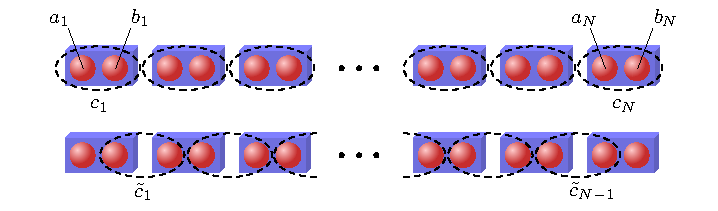
\includegraphics[width=\textwidth]{./figures/kitaev-chain.pdf}
  \caption{The top chain represents the system in a trivial topology where each complex fermion $c_j = \tfrac{1}{2}(a_j + i b_j)$ is a linear combination of intraconnected MFs. The bottom chain represents the system in a non-trivial topology where each complex fermion $\tilde{c}_j = \tfrac{1}{2}(a_j + i b_{j+1})$ is a linear combination of interconnected MFs, leaving the non-localized complex fermion $f = \tfrac{1}{2}(a_0 + i b_N)$, and thus leaving one MF located at each end of the chain.}
  \label{fig:kitaev-chain}
\end{figure}

Slightly outside the Kitaev limit, a non-trivial topology persists if $|\mu| < 2t$ and $t = |\Delta| >0$.
Due to bulk-edge correspondence, MZMs are localized at the interface between trivial and non-trivial segments.
To formalize this, we calculate the topological invariant, known as the Majorana number.
While calculating the Majorana number is straight forward enough, its proof on the other hand is not, this can be found in App. \ref{app:majorana-number}.
To compute the Majorana number, we perform a MF basis transformation on the Hamiltonian, $A = -iU \ham U^{\dagger}$, then take the sign of the Pfaffian,

\begin{equation}
  \mathcal{M} = \text{sgn} [\text{Pf} (A)].
\end{equation}
If the system has translational symmetry in $x$ and $y$, the Hamiltonian can be transformed into momentum space.
Using the symmetry condition $\epsilon(-k) = -\epsilon(k)$, we find that for any given $k$, there are equal numbers of positive and negative eigenvalues.
The Majorana numver then simplifies to

\begin{equation}
  \mathcal{M} =
  \begin{cases}
    \text{sgn} [\text{Pf} (A_{k=0}) \text{Pf} (A_{k=\pi})], &\text{if L is even}, \\
    \text{sgn} [\text{Pf} (A_{k=0})], &\text{if L is odd},
  \end{cases}
\end{equation}
where L is the number of lattice sites.
Within the Kitaev limit, if $|\mu|< 2t$, then $\mathcal{M} = -1$, and if $|\mu| > 2t$, then $\mathcal{M} = 1$.
If one section of the material exhibits non-trivial topology while adjacent sections remain trivial, MZMs will localize at interfaces of differing topological numbers.
This phenomena is a direct consequence of bulk-edge correspondence.

Now that we have a way to distinguish topological states, we must consider the size of the systems band gap and robustness.
When $|\mu| = 2t$, the system reaches a critical point where the band gap opens and closes, making this region of parameter space undesirable.
The band gap is too small, allowing even minor local perturbations to reopen or close the gap, which compromises the stability and information of the MZMs.
By tuning the chemical potential further from these critical points, the band gap enhances, increasing robustness against local perturbations (providing greater topological protection) ~\cite{kitaevUnpairedMajoranaFermions2001}.

\subsection{Half-quantum vortices in \textit{p}-wave superconductors}
We now transition to Ivanov's derivation of MFs and introduce \textit{braiding} for its topological quantum computing applications.
It was proposed by Read and Green that the Pfaffian quantum Hall state derived by Moore and Read belongs to the same topological class as the Bardeen-Cooper-Schrieffer (BCS) pairing state.
Ivanov later verified this was the case for a BCS-paired state, demonstrating that the Pfaffian state exhibits non-Abelian statistics in the presence of half-quantum vortices.
Since \textit{p}-wave superconductors share this topological structure, they also support non-Abelian statistics.
To answer this, we need to understand how the superconducting order parameter acts under different pairing potentials composed of singlet or triplet states ~\cite{ivanovNonAbelianStatisticsHalfQuantum2001}.

The superconducting order parameter, also called order parameter or pairing potential for short, tells us the correlation between two fermionic operators in a superconductor and requires the state to be antisymmetric.
The order parameter is made up of a spatial and spin component, with symmetry constraints dictating their relationship.
In spin-singlet pairing, the spin component is antisymmetric, limiting the spatial component to be symmetric.
This occurs in \textit{s}- and \textit{d}-wave superconductors.
In spin-triplet pairing, the spin component is symmetric, limiting the spatial component to be antisymmetric.
This occurs in \textit{p}- and \textit{f}-wave superconductors.

In terms of Pauli matrices, the order parameter can be expressed as

\begin{equation}
  \Delta (\vec{k}) = \left(\Delta_0 (\vec{k}) + \vec{d}(\vec{k}) \cdot \bm{\sigma}\right) i \sigma_y,
\end{equation}
where the antisymmetric condition $\Delta(\vec{k}) = \Delta^T(-\vec{k})$ enables $\Delta_0 (\vec{k})$ represents spin-singlet components and $\vec{d}(\vec{k})$ encodes spin-triplet components, and $\sigma_y$ maintains the overall antisymmetric nature of the matrix.
The direction vector $\vec{d}$ must be a three dimensional vector to ensure the three spin configurations
$|\uparrow\uparrow\rangle$, $|\uparrow\downarrow\rangle + |\downarrow\uparrow\rangle$, and $|\downarrow\downarrow\rangle$.
The parity of the spatial component determines $\Delta(\vec{k})$.
Even-parity is of even powers in momentum, proportional to even spherical harmonics.
Odd-parity is of odd powers in momentum, proportional to odd spherical harmonics.
For example, in \textit{s}-wave superconductors $l=0$, the spherical harmonic $Y_{0,0}$ is constant and has no momentum dependence and takes the form
$\Delta_s (\vec{k}) = i\Delta_0 \sigma_y$.
In contrast, for \textit{p}-wave superconductors $l=1$, the spherical harmonic $Y_{1,\pm1} \propto k_x \pm i k_y$, leading to linear dependence in momentum.
This leads to the order parameter
$\Delta_p(\vec{k}) = i\Delta (\vec{d} \cdot \bm{\sigma}) (k_x+ik_y) \sigma_y$.
This shows symmetry of the superconducting state determines the structure of $\Delta(\vec{k})$ and how it influences the physical properties of the system ~\cite{ivanovNonAbelianStatisticsHalfQuantum2001}.

\begin{figure}
  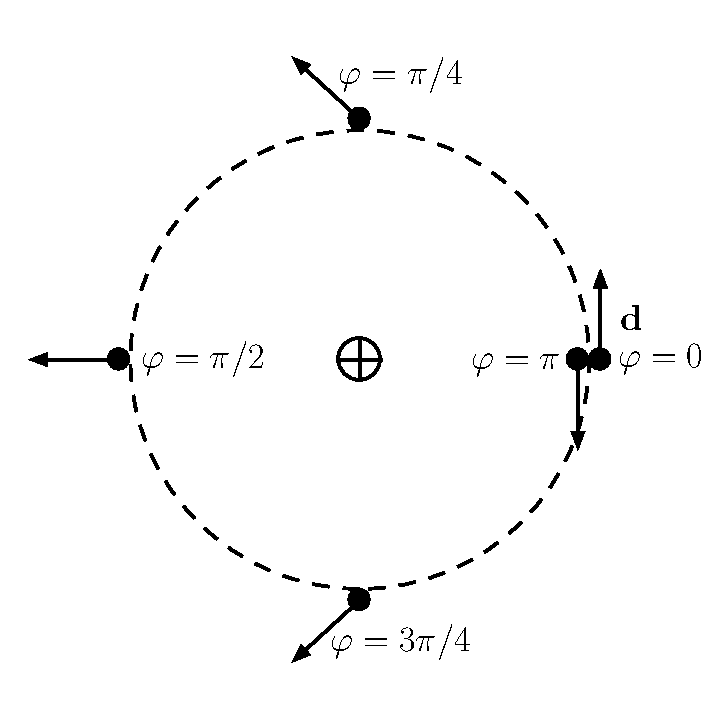
\includegraphics[width=0.4\textwidth]{./figures/half-quantum-vortex.pdf}
  \caption{The order phase $\varphi$ and angle $\alpha$ of $\vec{d}$ rotate by $\pi$: ($\varphi , \vec{d}$) \rightarrow ($\varphi+\pi, -\vec{d}$). The order parameter $\theta$ maps to itself, ($0, 2\pi$), under simultaneous change of both $\vec{d}$ and $\varphi$: $\theta = \varphi + \alpha$.}
  \label{fig:half-quantum-vortex}
\end{figure}

In Ivanov's proof, a slightly different basis for the triplet-pairing order parameter is used

\begin{equation}
  %\Delta (\vec{k}) = \Delta e^{i\phi} \left[ d_x \left(|\uparrow\uparrow\rangle + |\downarrow\downarrow\rangle \right) +i d_y \left(|\uparrow\uparrow\rangle - |\downarrow\downarrow\rangle \right) + d_z \left(|\uparrow\downarrow\rangle + |\downarrow\uparrow\rangle \right) \right] (k_x + i k_y),
  \Delta (\vec{k}) = \Delta e^{i\varphi} \left[ d_x \sigma_0 + i d_y \sigma_z + d_z \sigma_x \right] (k_x + i k_y),
\end{equation}
and follows the antisymmetric definition $\Delta(\vec{k}) = -\Delta^T (-\vec{k})$.
For a half-quantum vortex to exist, we must allow $\vec{d}$ to rotate in 3D or in a plane.
Additionally, the order parameter maps to itself, which requires the change of sign of $\vec{d}$ and shift in the phase $\varphi$ by $\pi$, simultaneously.
This mapping is
$(\varphi, \vec{d}) \mapsto (\varphi+\pi,-\vec{d})$
and can be seen in Figure ~\ref{fig:half-quantum-vortex} ~\cite{ivanovNonAbelianStatisticsHalfQuantum2001}.

We now reduce to a 2D superconductor, this forces $\vec{d}$ to point and rotate in the x-y plane and removes the coupling of spin-up and -down fermions from the order parameter.
The order parameter can then be written in polar coordinates

\begin{align}
  \Delta (\vec{k},r,\theta) &= \Delta(r) e^{i\varphi}
  \begin{bmatrix}
    e^{i\alpha} & 0 \\
    0 & e^{-i\alpha}
  \end{bmatrix}
  (k_x + i k_y) \nonumber \\
  &= \Delta(r)
  \begin{bmatrix}
    e^{i\theta} & 0 \\
    0 & 1
  \end{bmatrix}
  (k_x + i k_y),
\end{align}
where $\alpha$ is the angle of $\vec{d}$, remembering its simultaneous change w.r.t. $\varphi$.
We see that the spin-up fermions have a vortex while the spin-down do not have a vortex (and thus no low energy states).
The Hamiltonian for spin-up or spinful fermions can now be described by

\begin{equation}
  \ham = \int d^2 \vec{r} \left[ -\Psi^{\dagger} \left( \dfrac{\nabla^2}{2m} + \epsilon_F \right) \Psi + \Psi^{\dagger} \left[ e^{i\theta} \Delta(r) * \left( \partial_x +i\partial_y \right) \right] \Psi^{\dagger} + h.c. \right],
\end{equation}
where $*$ is the symmetrized product
[$A*B = (AB + BA) / 2$].
One can diagonlize the Hamiltonian using the quasiparticle operator
$\gamma^{\dagger} = u\Psi^{\dagger} + v\Psi$.
The creation annihilation of the same fermion is related by the parameters $u$ and $v$, causing the energy eigenstates to be symmetric about zero-energy, restricting
$\gamma^{\dagger}(E) = \gamma (E)$.
%It then leads to the zero-energy eigenstate being self-conjugate, a Majorana fermion, $\gamma^{\dagger}(E=0) = \gamma (E=0)$.
The spinful nature eliminates the spin degree of freedom and shows the creation and annihilation operators are coupled due to superconductivity, making MFs possible through self-conjugacy ~\cite{ivanovNonAbelianStatisticsHalfQuantum2001}.

\subsection{Braiding}
To speak on braiding it is important to start with gauge symmetry.
Under \textit{U}(1) gauge transformation, if the superconducting gap is shifted by $\phi$, it is the same as rotating the creation annihilation operator by half the shift.
Thus, $\Psi_{\alpha} \mapsto e^{i\phi/2} \Psi_{\alpha}$, which leads to the MF operator weights transforming as $(u,v) \mapsto (ue^{i\phi/2}, v^{-i\phi/2})$.
We can see with a change of superconducting order parameter by $2\pi$ the MF changes sign, $\gamma \mapsto -\gamma$ ~\cite{ivanovNonAbelianStatisticsHalfQuantum2001}.

\begin{figure}
  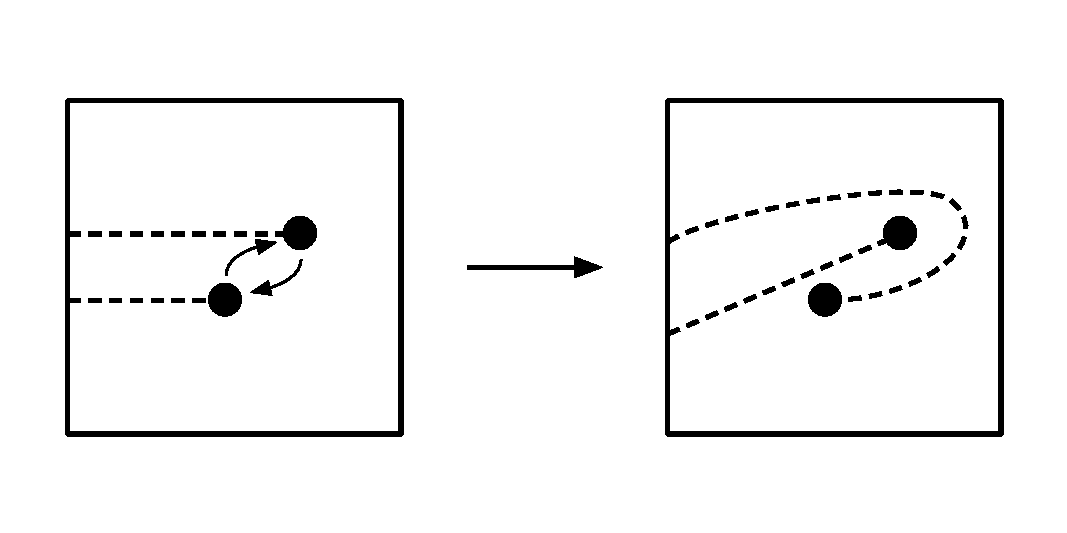
\includegraphics[width=0.5\textwidth]{./figures/pwave-braid.pdf}
  \caption{Two vortices in an elementary braid exchange.}
  \label{fig:pwave-braid}
\end{figure}


This change of sign is important in braiding transformations since it allows for non-Abelian exchange statistics.
We can circumvent a global phase by introducing branch cuts for the vortices to cross, causing a $2\pi$ phase change in the MFs.
Vortices can be exchanged as described in Figure ~\ref{fig:pwave-braid}, with a "bird's eye" view.
We can define the braiding operators as the following

\begin{equation}
  T_i :
  \begin{cases}
    \gamma_i \mapsto \gamma_{i+1} \\
    \gamma_{i+1} \mapsto -\gamma_i \\
    \gamma_j \mapsto \gamma_j \quad\quad \text{for $j\neq i$ and $j\neq i+1$}.
  \end{cases}
\end{equation}
This leads to the following braiding relations

\begin{figure}
  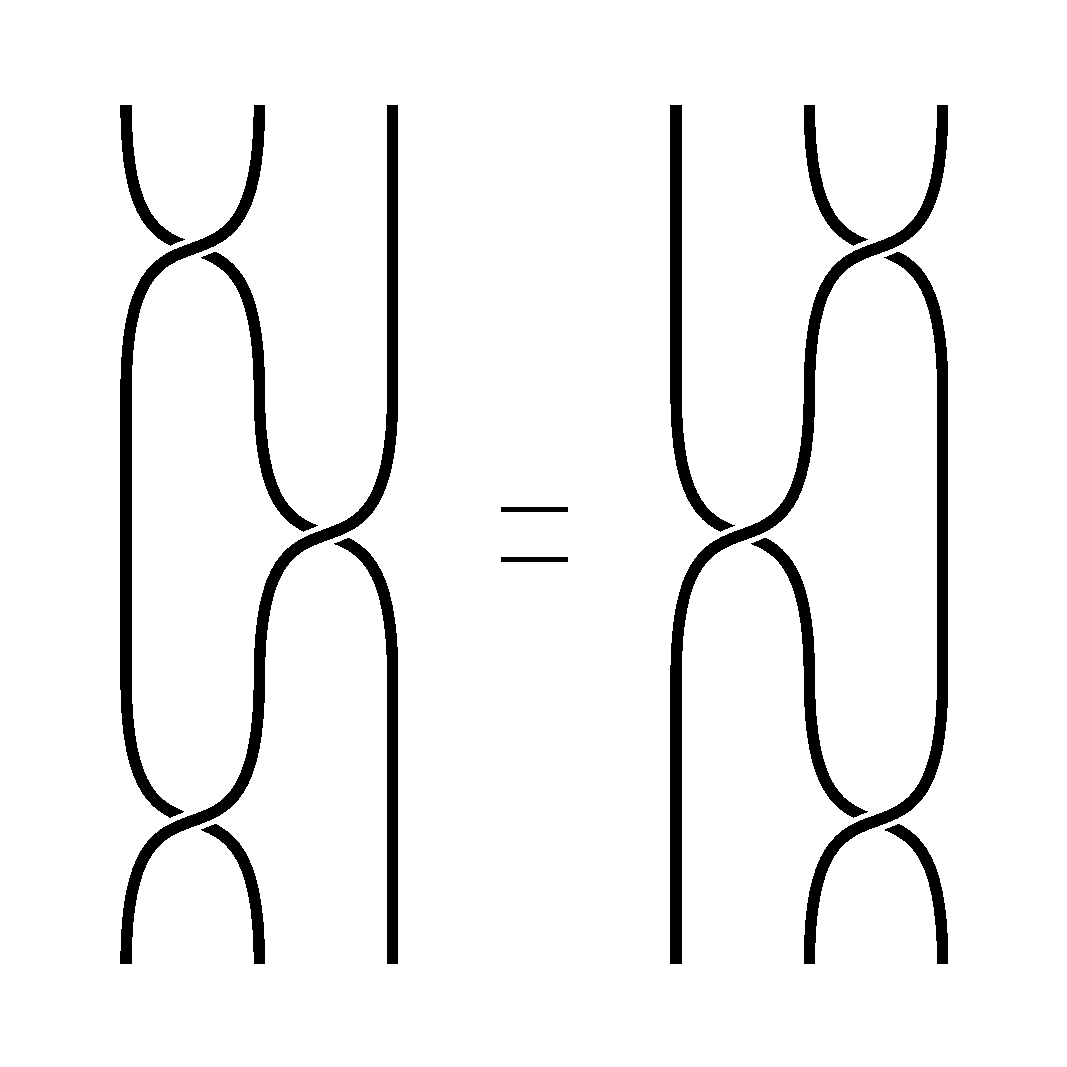
\includegraphics[width=0.33\textwidth]{./figures/braid.pdf}
  \caption{Braid group relation for $T_i T_{i+1} T_i = T_{i+1} T_i T_{i+1}$.}
  \label{fig:braid}
\end{figure}
\begin{equation}
  \begin{align*}
    T_i T_j = T_j T_i, \quad |i-j| > 1, \\
    T_i T_j T_i = T_j T_i T_j, \quad |i-j| = 1.
  \end{align*}
\end{equation}
Figure ~\ref{fig:braid} demonstrates three neighboring vortices with braiding statistics having two means of achieving the same braiding exchange.
One can write the braiding operators in terms of fermionic operators with the following

\begin{equation}
  \tau(T_i) = \exp\left(\dfrac{\pi}{4} \gamma_{i+1} \gamma_i\right) = \dfrac{1}{\sqrt{2}} \left(1+ \gamma_{i+1} \gamma_i\right).
\end{equation}
This can be further carried out for any number of MFs and builds a set of braiding operators for that system ~\cite{ivanovNonAbelianStatisticsHalfQuantum2001}.

\begin{figure}[t]
  \begin{tikzpicture}
    \node[inner sep=0pt] (f1) at (-3,0) {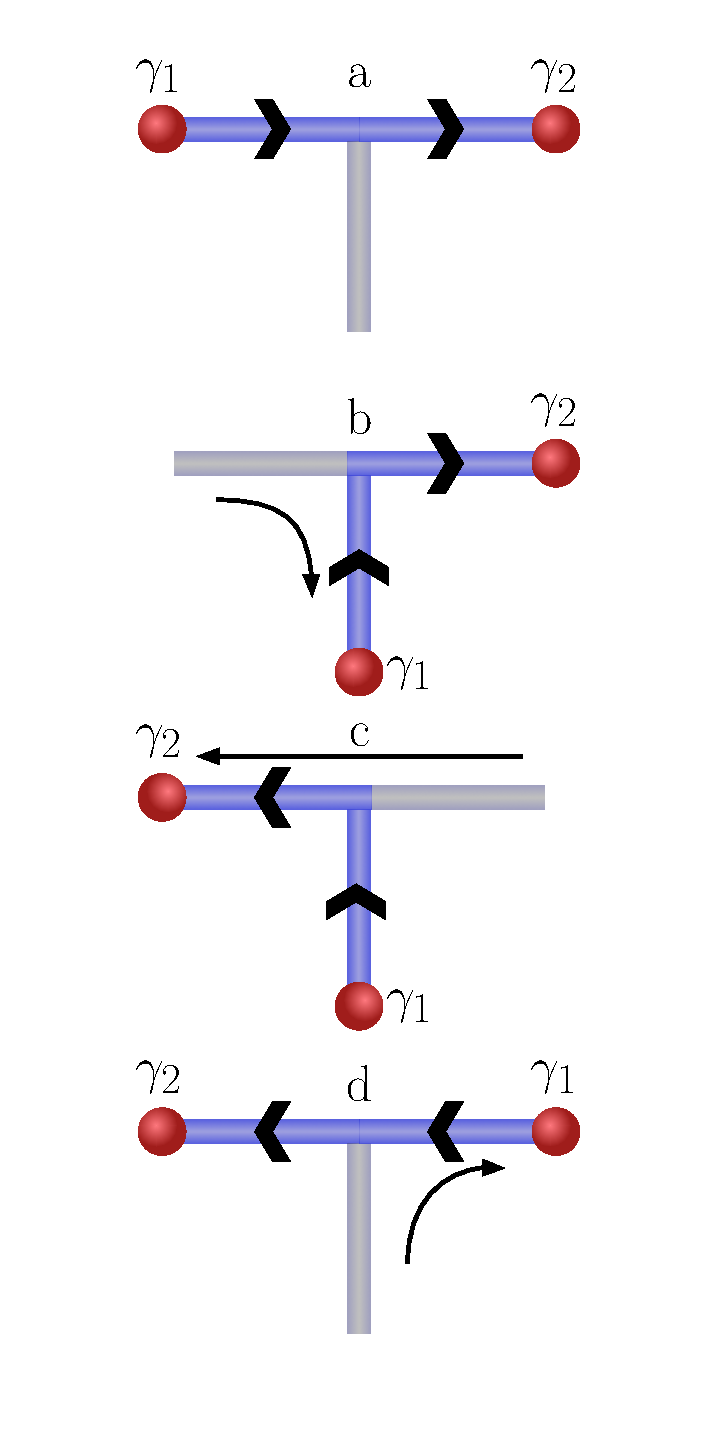
\includegraphics[width=0.25\textwidth]{./figures/t-junction-braid.pdf}};
    \node[inner sep=0pt] (f2) at (3,0) {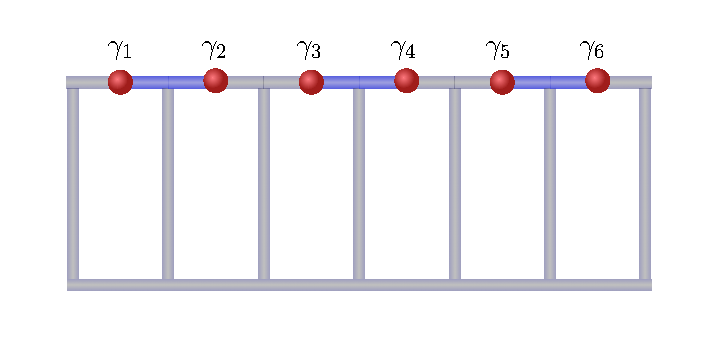
\includegraphics[width=0.5\textwidth]{./figures/ladder-junction.pdf}};
  \end{tikzpicture}
  \caption{(Left) Braiding two MFs on a T-junction. (Right) Ladder junction schematic for hosting and braiding multiple MFs.}
  \label{fig:t-junction-braid}
\end{figure}

\subsection{T-junction qubit}
The simplest qubit theorized for braiding MFs is on 1D wires connected in a T-junction, which can be extrapolated to a ladder junction for $2n$ MFs.
In the T-junction we define the quasi-1D Hamiltonian

\begin{equation}
  \ham = -\mu \sum_j \cc_j c_j - \sum_j \left(t\cc_j c_{j+1} + |\Delta|e^{i\phi} c_j c_{j+1} + h.c. \right),
\end{equation}
where
$c_j = e^{-i\phi/2} (\gamma_{j+1,1} + i \gamma_{j,2})/2$.
We additionally have to define the pairing as
$|\Delta|e^{i\phi} c_j c_{j+1}$
such that the site indices have the following definitions
\begin{itemize}
  \item Increase moving $\rightarrow / \uparrow$ in the horizontal/vertical wires: $\phi = 0$,
  \item Decrease moving $\leftarrow / \downarrow$ in the horizontal/vertical wires: $\phi = \pi$.
\end{itemize}
The braiding of two MFs in a T-junction is achieved by adiabatically tuning the voltage gate, or chemical potential, of the wires which can be seen in Figure ~\ref{fig:t-junction-braid}.
Then, extrapolate to a ladder junction as shown in Figure ~\ref{fig:t-junction-braid} ~\cite{aliceaNonAbelianStatisticsTopological2011}.
While this approach is simple in theory and being seriously pursued, it is difficult to build, manipulate, and read experimentally.
Another difficulty for these wires is due to not having any truly \textit{p}-wave superconductors, currently they need to be built from heterostructures to make an effective \textit{p}-wave superconductor.


\begin{enumerate}
  \item \Blue{Braiding (Application in TQC)}
    not sure how much to talk about here, and slightly mentioned earlier with topological superconductors.
\end{enumerate}

\section{Landau levels and quantum Hall effect}

\subsection{Landau levels in condensed matter systems}
We are interested in using non-uniform circularly polarized laser light to induce QHE in 2DEG and Dirac systems and determine whether the energy levels are Landau level-like (LLL).
In the classical case of charged QHE the charged particles in the system are quantized in cyclotron orbits due to perpendicular magnetic field, these energies are called Landau levels (LLs).
To understand why LLs appear and QHE arises we need to first solve the Hamiltonian associated with a 2DEG and Dirac systems in the presence of a perpendicular magnetic field.
We can start with the square lattice tight-binding Hamiltonian for a 2DEG

\begin{equation}
  \ham = -\sum_{\langle j,l \rangle} t\cc_j c_{l} + h.c.,
\end{equation}
and in momentum space

\begin{equation}
  \ham = -\sum_{\vec{p}} 2t \left( \cos{(p_x a)} + \cos{(p_y a)} \right) \cc_{\vec{p}} c_{\vec{p}}.
\end{equation}
Then in the limit of small momenta $p$ we arrive at

\begin{align}
  \ham &= -\sum_{\vec{p}} 2t \left( 2 - \dfrac{p_x^2a^2}{2} -\dfrac{p_y^2a^2}{2} \right) \cc_{\vec{p}} c_{\vec{p}}, \nonumber \\
  \ham(\vec{p}) &= \dfrac{p_x^2 + p_y^2}{2m},
\end{align}
we have thus arrived at Schrodingers equation for a 2DEG in the limit of small momenta.
Let us assume a 2DEG in the $x$-$y$ plane and has a magnetic field that points in the positive $\hat{z}$ direction, $\vec{B} = B\hat{z}$ or $\vec{A} = Bx\hat{y}$.
The Hamiltonian in momentum space then becomes

\begin{equation}
  \ham = \dfrac{1}{2m} \left( \op{p}_x^2 + (\op{p}_y - qB \op{x})^2 \right)
\end{equation}
Recall $[\op{r}_{\alpha}, \op{p}_{\beta}] = i\hbar \delta_{\alpha,\beta}$, that means our magnetic term commutes with $\op{p_y}$, so let us assume that $\Psi(x,y) = e^{ik_y y} \psi(x)$.
Acting the Hamiltonian on the ansatz wavefunction yields

\begin{align}
  \ham\Psi &= \dfrac{1}{2m} \left( \op{p}_x^2 + (qB \op{x} - \hbar k_y)^2 \right)e^{ik_y y} \psi(x) \nonumber \\
  \ham & = \dfrac{1}{2m} \left( \op{p}_x^2 + q^2 B^2 \op{x}^2 \right)
\end{align}
where we let $x - \tfrac{\hbar k_y}{qB} \rightarrow x$, since it is just a shift in $x$ coordinates.
Notice that we arrive at the expression for a quantum harmonic oscillator.
A derivation for the energy solutions can be found in \ref{appendix:qho}.
With the energy solutions

\begin{equation}
  E_n = \dfrac{\hbar q B}{m} \left(n+\dfrac{1}{2}\ \right) = \hbar \omega \left(n + \dfrac{1}{2} \right)
\end{equation}

An alteration to the lattice model can have slightly different results.
Using a honeycomb lattice, provided by graphene, gives the following Hamiltonian

\begin{equation}
  \ham = -t \sum_{\substack{j, l \\ \alpha \beta}} \cc_{j\alpha} c_{l\beta} + h.c.,
\end{equation}
with lattice vectors $\vec{a}_1 = \sqrt{3} a \hat{x}$ and $\vec{a}_2 = \tfrac{\sqrt{3}}{2} a \hat{x} + \tfrac{3}{2} a \hat{y}$.
In momentum space
\[
  \ham = -t \sum_{\vec{p}}
  \begin{bmatrix}
    0 & 1 + e^{i\vec{p}\cdot \vec{a}_1 } + e^{i \vec{p}\cdot \vec{a}_2} \\
    1 + e^{-i\vec{p}\cdot \vec{a}_1 } + e^{-i \vec{p}\cdot \vec{a}_2} & 0
  \end{bmatrix},
\]
\[
  \ham(\vec{p}) =
  \begin{bmatrix}
    0 & t(\vec{p}) \\
    t^*(\vec{p}) & 0
  \end{bmatrix},
\]
where the hopping can be rewritten as

\begin{equation}
  t(\vec{p}) = -t e^{i\sqrt{3} p_x a / 2} \left( 2\cos{\left( \dfrac{\sqrt{3} p_x a }{ 2 } \right)} + e^{i 3 p_y a /2 } \right)
\end{equation}
which gives the following energy spectrum

\begin{equation}
  E(\vec{p}) = \pm t \sqrt{3 + 2\cos{\left(\sqrt{3}p_x a\right)} + 4\cos{\left(\dfrac{\sqrt{3}p_x a}{2}\right)}\cos{\left(\dfrac{3p_y a}{2}\right)} }.
\end{equation}
There are several high symmetry points on the corners of the Brillouin zone, one such point is $\vec{K} = \tfrac{4\pi}{3\sqrt{3}a} \hat{x} $.
Going back to the Hamiltonian and expanding about $\vec{K}$ with small $\vec{q}$, $\vec{q} = \vec{p} + \vec{K}$, gives the following hopping amplitude

\begin{align}
  t(\vec{q}) &= -t e^{i\sqrt{3} q_x a / 2} e^{i\sqrt{3} K a / 2} \left( 2\cos{\left( \dfrac{\sqrt{3} q_x a }{2}  + \dfrac{\sqrt{3} K a}{2} \right)} + e^{i 3 p_y a /2 } \right) \nonumber \\
  %t(\vec{q}) &= -t e^{i\sqrt{3} q_x a / 2} e^{i 2\pi/3} \left( 2\cos{\left( \dfrac{\sqrt{3} q_x a }{2}  + \dfrac{2\pi}{3} \right)} + e^{i 3 p_y a /2 } \right) \nonumber \\
  %t(\vec{q}) &= -t e^{i\sqrt{3} q_x a / 2} e^{i 2\pi/3} \left( -\cos{\left( \dfrac{\sqrt{3} q_x a }{2}\right)} - \sqrt{3}\sin{\left( \dfrac{\sqrt{3}q_x a}{3} \right)} + e^{i 3 p_y a /2 } \right) \nonumber \\
  %t(\vec{q}) &\approx t e^{i 2\pi/3} \left(\dfrac{3q_x a}{2} - \dfrac{i3q_y a}{2} \right) \nonumber \\
\end{align}
and in the small momenta $q$ limit
\begin{align}
  t(\vec{q}) &\approx v_F e^{i 2\pi/3} \left(q_x - iq_y \right), \nonumber \\
  t^*(\vec{q}) &\approx v_F e^{-i 2\pi/3} \left(q_x + iq_y \right), \nonumber
\end{align}
where we keep the leading order in $\vec{q}$ and $v_F = \tfrac{3ta}{2}$.
Using a gauge transformation and redefining $\vec{q} \rightarrow \vec{p}$ we arrive at the Dirac equation

\begin{equation}
  \ham(\vec{p}) = v_F \bm{\sigma}\cdot \vec{p}.
\end{equation}
With graphene spanning the $x$-$y$ plane in the presence of a magnetic field $\vec{B} = B\hat{z}$, $\vec{A} =  Bx\hat{y}$, the Dirac equation becomes

\begin{equation}
  \ham(\vec{p}) = v_F \bm{\sigma}\cdot \left(\vec{p} - q\vec{A} \right).
\end{equation}
A derivation for the energy solution can be found in \ref{appendix:dirac}.
The quantized energy solutions for a 2D Dirac equation in the presence of perpendicular magnetic field is

\begin{equation}
  E_n = v_F \sqrt{2 n \hbar qB }
\end{equation}

We see the energy of both systems produce discrete quantized energies for charged particles in cyclotron orbits with no depenedence on momenta, these are Landau levels.
It is also important to note these Landau levels are highly degenerate flat bands, which will lend to the discussion of bulk insulating states.

\subsection{Quantized Hall conductivity and Chern number}

Here we will go over the relationship between quantized Hall conductivity and Chern number, which is described as

\begin{equation}
  \sigma_{xy} = - C\dfrac{e^2}{h}, \quad C \in \mathbb{Z}.
\end{equation}
Let us consider a 2D system with translation symmetry in the $x$ and $y$ axis with lattice constants $l_x$ and $l_y$, respectively.
The Brillouin zone boundaries are
\begin{equation}
  k_x = \dfrac{\pi}{l_x} [-1,1) \quad \text{and} \quad k_y = \dfrac{\pi}{l_y} [-1,1),
\end{equation}
where we can think of the periodicity in $k_x$ and $k_y$ creating a torus, $\vec{T}$, in 3D space.
We now introduce the Kubo formula, which is a linear response to a physical observable by a time-dependent perturbation, for conductivity as

\begin{equation} \label{eq:kubo}
  \sigma_{xy} = i\hbar \sum_{E_a < E_F < E_b} \int_{\vec{T}} \dfrac{d^2k}{(2\pi)^2} \dfrac{\langle u_{\vec{k}}^a | J_y | u_{\vec{k}}^b \rangle \langle u_{\vec{k}}^b | J_x | u_{\vec{k}}^a \rangle - \langle u_{\vec{k}}^a | J_x | u_{\vec{k}}^b \rangle \langle u_{\vec{k}}^b | J_y | u_{\vec{k}}^a \rangle}{{(E_b - E_a)}^2}.
\end{equation}
The $a$ and $b$ terms represent dispersion bands below and above the Fermi energy, respectively, and a basic requirement the bands be separated to allow for an insulator.
Recall, current density can be defined by $\vec{J} = (e/\hbar) \partial_{\vec{k}} H$.
So long as $H$ is written in a basis that current density is non-zero we can continue.
Plugging current density in Eq. \eqref{eq:kubo} gives

\begin{equation}
  \sigma_{xy} = \dfrac{ie^2}{h} \sum_{E_a < E_F < E_b} \int_{\vec{T}} \dfrac{d^2k}{2\pi} \dfrac{\langle u_{\vec{k}}^a | \partial_{k_y} H | u_{\vec{k}}^b \rangle \langle u_{\vec{k}}^b | \partial_{k_x} H | u_{\vec{k}}^a \rangle - \langle u_{\vec{k}}^a | \partial_{k_x} H | u_{\vec{k}}^b \rangle \langle u_{\vec{k}}^b | \partial_{k_y} H | u_{\vec{k}}^a \rangle}{{(E_b - E_a)}^2}.
\end{equation}
Using the product rule on the following expression $\langle \alpha | \partial_j (H | \beta\rangle)$ and using $\sum_b = \vec{1} - \sum_a |u_{\vec{k}}^a\rangle \langle u_{\vec{k}}^a |$ lets us simplify the previous expression to

\begin{equation}
  \sigma_{xy} = \dfrac{e^2}{h} \sum_{a} \int_{\vec{T}} \dfrac{d^2k}{2\pi} i\left(\langle \partial_{k_y} u_{\vec{k}}^a | \partial_{k_x} u_{\vec{k}}^a \rangle - \langle \partial_{k_x} u_{\vec{k}}^a | \partial_{k_y} u_{\vec{k}}^a \rangle \right) = \dfrac{e^2}{h} \sum_{a} \int_{\vec{T}} \dfrac{d^2k}{2\pi} \mathcal{F}_{xy}
\end{equation}
where we recognize the integral is the negative Chern number integral, which is always integer.
The Hall conductivity becomes

\begin{equation}
  \sigma_{xy} = -\dfrac{e^2}{h} \sum_a C_a = -C \dfrac{e^2}{h}.
\end{equation}
This leads to Hall conductivity becoming quantized and increases as the Fermi energy fills more bands.
This is one way to describe the topological invariant of the quantum Hall effect by looking at geometry of momentum space with PBC.

\subsection{Laughlin pump on a Hall cylinder}
We demonstrate another way to describe quantum Hall effect for Landau Levels on a Hall cyclinder.
For a 2D system we let there be PBC in the $y$-axis with length $L$, which discretizes momentum space into $k = 2\pi n/ L$ points.
This creates a cylinder with the $y$ in the angular axis and $x$ in the axial axis.
Laughlin pumping requires one apply a flux along the cyclinder's $x$ axis.
We can introduce the flux in the gauge potential as

\begin{equation}
  \vec{A} = (Bx + \Phi/L)\hat{y}.
\end{equation}
Inserting the flux into the LL Schrodinger Hamiltonian gives

\begin{equation}
  \ham = \dfrac{1}{2m^*} \left( p_x^2 + {\left(\dfrac{2\pi \hbar n}{L} + eBx + \dfrac{e\Phi}{L} \right)}^2\right).
\end{equation}
This becomes the quantum harmonic oscillator solution we saw earlier where we let $x' = x + x_n$ and

\begin{equation} \label{eq:xCM}
  x_n = \dfrac{h}{eBL} \left(n + \dfrac{\Phi}{\Phi_0} \right),
\end{equation}
where $\Phi_0 = h/e$ is the flux quanta.
The generalized LL wave function solution is

\begin{equation}
  \psi_n(x) \propto H_n (x+x_n) e^{-eB(x+x_n)^2 / 2\hbar} e^{i2\pi n/L},
\end{equation}
where $H_n(x)$ is the Hermite polynomial.
Solving for $\langle x_n \rangle = \langle \psi_n(x) | x | \psi_n(x) \rangle$ we see each electron is centered at Eq. \eqref{eq:xCM}.

When the flux increments by one flux quanta we notice each electron's center of mass moves by the same integer multiple, i.e.\ the states go from $n\rightarrow n+1$.
This is a change in charge as electrons are pumped from one state to the next, or from one edge of the cyclinder to the other.
If $n$ LLs are filled then $n$ electrons are transferred, as $\Delta Q = ne$.
The Hall conductivity can be written as $\sigma_H = \Delta Q / \Delta \Phi$.
After a change in flux $\Delta \Phi = \Phi_0$ the Hall conductivity is quantized as $\sigma_H = ne^2 / h$.
Once again we have shown Hall conductivity is quantized for LL systems.


\item \Blue{Landau Level and Hofstadter butterfly}
\begin{enumerate}[i]
  \item \Blue{solve for LL in 2DEG --- why it's topological, chern number, TKNN quantum Hall}
  \item \Blue{square lattice --- hofstadter butterfly ( on other lattices, honeycomb)}
\end{enumerate}


\chapter{Superconducting Triangular Islands as a Platform for Manipulating Majorana Zero Modes}

\section{Introduction}

For more than twenty years, Majorana zero modes (MZM) in condensed matter systems have been highly sought after due to their potential for serving as building blocks of topological quantum computation, thanks to their inherent robustness against decoherence and non-Abelian exchange statistics \cite{ivanovNonAbelianStatisticsHalfQuantum2001, kitaevFaulttolerantQuantumComputation2003, nayakNonAbelianAnyonsTopological2008, aliceaNonAbelianStatisticsTopological2011, aasenMilestonesMajoranaBasedQuantum2016}. MZM were originally proposed to be found in half-quantum vortices of two-dimensional (2D) topological \textit{p}-wave superconductors and at the ends of 1D spinless \textit{p}-wave superconductors \cite{readPairedStatesFermions2000, kitaevUnpairedMajoranaFermions2001}. Whether a pristine \textit{p}-wave superconductor \cite{brisonPWaveSuperconductivityDVector2021} has been found is still under debate. However, innovative heterostructures proximate to ordinary $s$-wave superconductors have been proposed to behave as effective topological superconductors in both 1D and 2D. These include, for example, semiconductor nanowires subject to magnetic fields \cite{mourikSignaturesMajoranaFermions2012, rokhinsonFractionalJosephsonEffect2012, dengAnomalousZeroBiasConductance2012}, ferromagnetic atomic spin chains \cite{choyMajoranaFermionsEmerging2011, brauneckerInterplayClassicalMagnetic2013, klinovajaTopologicalSuperconductivityMajorana2013,nadj-pergeProposalRealizingMajorana2013,nadj-pergeObservationMajoranaFermions2014,schneiderPrecursorsMajoranaModes2022}, 3D topological insulators \cite{fuSuperconductingProximityEffect2008, hosurMajoranaModesEnds2011, potterEngineeringMathitipSuperconductor2011, veldhorstMagnetotransportInducedSuperconductivity2013}, quantum anomalous Hall insulators \cite{chenQuasionedimensionalQuantumAnomalous2018, zengQuantumAnomalousHall2018, xieCreatingLocalizedMajorana2021}, quasi-2D spin-orbit-coupled superconductors with a perpendicular Zeeman field \cite{oregHelicalLiquidsMajorana2010, sauGenericNewPlatform2010, lutchynSearchMajoranaFermions2011, potterTopologicalSuperconductivityMajorana2012, liTwodimensionalChiralTopological2016, leiUltrathinFilmsSuperconducting2018}, and planar Josephson junctions \cite{black-schafferMajoranaFermionsSpinorbitcoupled2011, pientkaSignaturesTopologicalPhase2013, hellTwoDimensionalPlatformNetworks2017, fornieriEvidenceTopologicalSuperconductivity2019, renTopologicalSuperconductivityPhasecontrolled2019, scharfTuningTopologicalSuperconductivity2019, zhouPhaseControlMajorana2020}, etc. It has been a challenging task to decisively confirm the existence of MZM in the various experimental systems due to other competing mechanisms that can potentially result in similar features as MZM do in different probes \cite{xuExperimentalDetectionMajorana2015, albrechtExponentialProtectionZero2016, sunMajoranaZeroMode2016, wangEvidenceMajoranaBound2018, jackObservationMajoranaZero2019, fornieriEvidenceTopologicalSuperconductivity2019, renTopologicalSuperconductivityPhasecontrolled2019, mannaSignaturePairMajorana2020}. Other proposals for constructing Kitaev chains through a bottom-up approach, based on, e.g. magnetic tunnel junctions proximate to spin-orbit-coupled superconductors \cite{fatinWirelessMajoranaBound2016}, and quantum dots coupled through superconducting links \cite{sauRealizingRobustPractical2012,leijnseParityQubitsPoor2012,dvirRealizationMinimalKitaev2023} are therefore promising. In particular, the recent experiment \cite{dvirRealizationMinimalKitaev2023} of a designer minimal Kitaev chain based on two quantum dots coupled through tunable crossed Andreev reflections (CAR) offers a compelling route towards MZM platforms based on exactly solvable building blocks.

In parallel with the above efforts of realizing MZM in different materials systems, scalable architectures for quantum logic circuits based on MZM have also been intensely studied over the past decades. A major proposal among these studies is to build networks of T-junctions, which are minimal units for swapping a pair of MZM hosted at different ends of a junction, that allow braiding-based TQC \cite{aasenMilestonesMajoranaBasedQuantum2016}. Alternatively, networks based on coupled wires forming the so-called tetrons and hexons, aiming at measurement-based logic gate operations  \cite{karzigScalableDesignsQuasiparticlepoisoningprotected2017}, have also been extensively investigated. To counter the technical challenges of engineering networks with physical wires or atomic chains, various ideas based on effective Kitaev chains, such as quasi-1D systems in thin films \cite{potterMultichannelGeneralizationKitaev2010}, cross Josephson junctions \cite{zhouPhaseControlMajorana2020}, scissor cuts on a quantum anomalous Hall insulator \cite{xieCreatingLocalizedMajorana2021}, and rings of magnetic atoms \cite{liManipulatingMajoranaZero2016}, etc. have been proposed. However, due to the same difficulty of obtaining or identifying genuine MZM in quasi-1D systems mentioned above, it remains unclear how practical these strategies are in the near future.

In this Letter, we propose an alternative structural unit for manipulating MZM, triangular superconducting islands, motivated by the above challenges associated with wire geometries and by the fact that triangular islands routinely appear spontaneously in epitaxial growth \cite{pietzschSpinResolvedElectronicStructure2006} on close-packed atomic surfaces. We first show that a minimal ``Kitaev triangle'' consisting of three sites hosts MZM at different pairs of vertices controlled by Peierls phases on the three edges [Fig.~\ref{fig:triangles} (a)], which can be readily realized using quantum dots. To generalize the minimal model to triangular structures involving more degrees of freedom, we study the topological phase transitions of quasi-1D ribbons driven by Peierls phases, which can be created by magnetic fields or supercurrents \cite{romitoManipulatingMajoranaFermions2012, takasanSupercurrentinducedTopologicalPhase2022}, and use the resulting phase diagram as a guide to construct finite-size triangles with a hollow interior that host MZM  [Fig.~\ref{fig:triangles} (b)]. In the end we discuss possible experimental systems that can realize our proposals and scaled-up networks of triangles for implementing braiding operations of MZM.



\section{Kitaev Triangle}

\begin{figure}[!ht]
  \hspace{-18pt}
  \subfloat[]{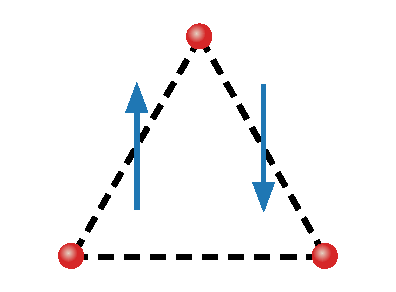
\includegraphics[width=3.0 in]{./figures/3-point-triangle.pdf}}
  \subfloat[]{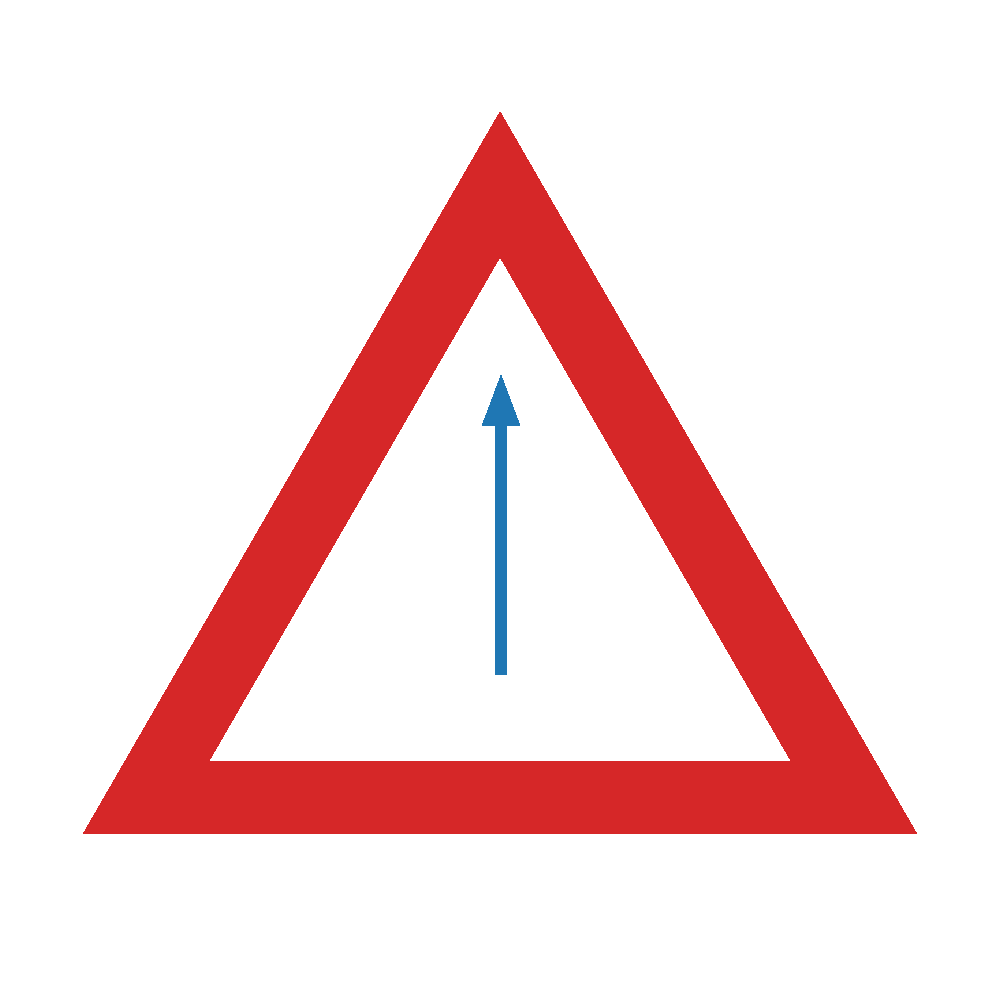
\includegraphics[width=2.4 in]{./figures/hollow-triangle-constant-vector-potential.pdf}}
  \caption{Schematics of two triangle structures proposed in this work. (a) Three-site Kitaev triangle with bond-dependent Peierls phases. (b) Hollow triangular island with a uniform vector potential.}
  \label{fig:triangles}
\end{figure}


In this section we present an exactly solvable minimal model with three sites forming a ``Kitaev triangle" that can host MZM at different pairs of vertices controlled by Peierls phases on the edges. The Bogoliubov-de Gennes (BdG) Hamiltonian includes complex hopping and $p$-wave pairing between three spinless fermions forming an equilateral triangle [Fig.~\ref{fig:triangles} (a)]:
\begin{equation}\label{eq:HBdG}
  \ham = \sum_{\langle j l \rangle} (-te^{i\phi_{jl}}\cc_{j} c_l + \de e^{i\theta_{jl}} c_{j} c_l + {\rm h.c.}) - \sum_{j} \mu \cc_j c_j,
\end{equation}
where $t$ is the hopping amplitude, $\de$ is the amplitude of the (2D) $p$-wave pairing, $\mu$ is the chemical potential, $\theta_{jl}$ is the polar angle of $\mathbf r_{jl} = \mathbf r_l - \mathbf r_j$ (the $x$ axis is chosen to be along $\mathbf r_{12}$), consistent with $\{c^\dag_l, c^\dag_j\} = 0$. $\phi_{jl}$ is the Peierls phase due to a bond-dependent vector potential $\mathbf A$ to be specified below (the nearest neighbor distance $a$ is chosen to be the length unit hereinbelow):
\begin{eqnarray}
\phi_{jl} = \dfrac{e}{\hbar} \int_{\mathbf r_j}^{\mathbf r_{l}} \vec{A} \cdot d\vec{l} = -\phi_{lj}
\end{eqnarray}
where $e>0$ is the absolute value of the electron charge. Below we use the natural units $e=\hbar=1$. To get the conditions for having MZM in this model we rewrite $\mathcal{H}$ in the Majorana fermion basis $a_{j} = c_j + c^\dag_j$, $b_j = \frac{1}{i}(c_j - c^\dag_j)$:
\begin{align}\label{eq:H3M}
    \ham =  -\dfrac{i}{2} \sum_{\langle j l \rangle} \Big[&\left(t\sin\phi_{jl}-\de\sin\theta_{jl}\right) a_j a_l \\\nonumber
  +&\left(t\sin\phi_{jl}+\de\sin\theta_{jl}\right) b_j b_l  \\\nonumber
  +&\left(t\cos\phi_{jl} - \de\cos\theta_{jl}\right) a_j b_l  \\\nonumber
  -&\left(t\cos\phi_{jl}+\de\cos\theta_{jl}\right) b_j a_l\Big]  -\dfrac{i\mu}{2} \sum_j  a_j b_j
\end{align}
For concreteness we consider the Kitaev limit $t=\de$, $\mu=0$, and choose $\phi_{12} = 0$ so that sites 1 and 2 alone form a minimal Kitaev chain with $\mathcal{H}_{12} = itb_1a_2$ and hosting MZM $a_1$ and $b_2$. In order for the MZM to persist in the presence of site 3, one can choose $\phi_{23}$ and $\phi_{31}$ so that all terms involving these Majorana operators cancel out. For example, consider the $2-3$ bond, for which $\theta_{23} = 2\pi/3$, we require
\begin{eqnarray}
    \sin\phi_{23} + \sin\frac{2\pi}{3} =\cos\phi_{23} + \cos\frac{2\pi}{3} = 0
\end{eqnarray}
which means $\phi_{23} = -\pi/3$. Similarly one can find $\phi_{31} =-\phi_{13} = -\pi/3$. The three Peierls phases can be realized by the following staggered vector potential
\begin{equation}\label{eq:Astep}
  \vec{A} =\left[1-2\Theta(x)\right]\frac{2 \pi}{3\sqrt{3}} \hat{y}
\end{equation}
where $\Theta(x)$ is the Heavisde step function. In fact, using a uniform $\vec{A} =\frac{2 \pi}{3\sqrt{3}} \hat{y}$, which corresponds to $\phi_{23} = -\pi/3 = -\phi_{31}$ also works, since the existence of $a_1$ is unaffected by $\phi_{23}$. However, in this case the counterpart of $b_2$ is not localized on a single site. For the same reason, the above condition for MZM localized at triangle corners can be generalized to Kitaev chains forming a triangular loop, as well as to finite-size triangles of 2D spinless $p$-wave superconductors in the Kitaev limit, as the existence of $a_1$ and $b_2$ are only dictated by the vector potential near the corresponding corners. It should be noted that in the latter case, 1D Majorana edge states will arise when the triangle becomes larger, and effectively diminish the gap that protects the corner MZM.  On the other hand, for the longer Kitaev chain, due to the potential practical difficulty of controlling further-neighbor hopping and pairing amplitudes, it is better to resort to the approach of controlling the individual topological phases of the three edges which will be detailed in the next section.

We next show that the minimal Kitaev triangle suffices to demonstrate braiding of MZM. To this end we consider a closed parameter path linearly interpolating between the following sets of values of $\phi_{jl}$:
\begin{eqnarray}
    (\phi_{12},\phi_{23},\phi_{31}) &=& \left(0,-\frac{\pi}{3},-\frac{\pi}{3}\right ) \equiv \bm \phi_1 \\\nonumber
    &\rightarrow& \left(-\frac{\pi}{3},-\frac{\pi}{3},0 \right) \equiv \bm \phi_2 \\\nonumber
    &\rightarrow& \left(-\frac{\pi}{3},0,-\frac{\pi}{3} \right) \equiv \bm \phi_3 \\\nonumber
    &\rightarrow& \bm \phi_1
\end{eqnarray}
It is straightforward to show that at $\bm \phi_{2}$ and $\bm \phi_3$ there are MZM located at sites $3,1$ and $2,3$, respectively. Therefore the two original MZM at sites $1,2$ should switch their positions at the end of the adiabatic evolution.

\begin{figure}[!ht]
	\centering
  \hspace{-27pt}
  \subfloat[]{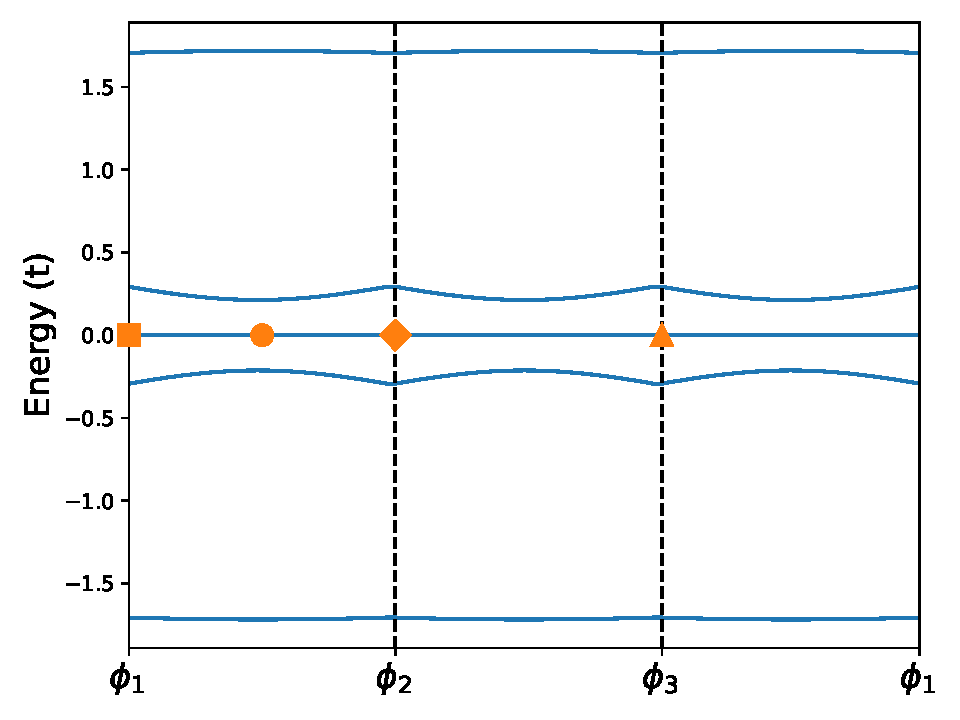
\includegraphics[width=3.3 in]{./figures/3eigval.pdf}}\\
  \subfloat[]{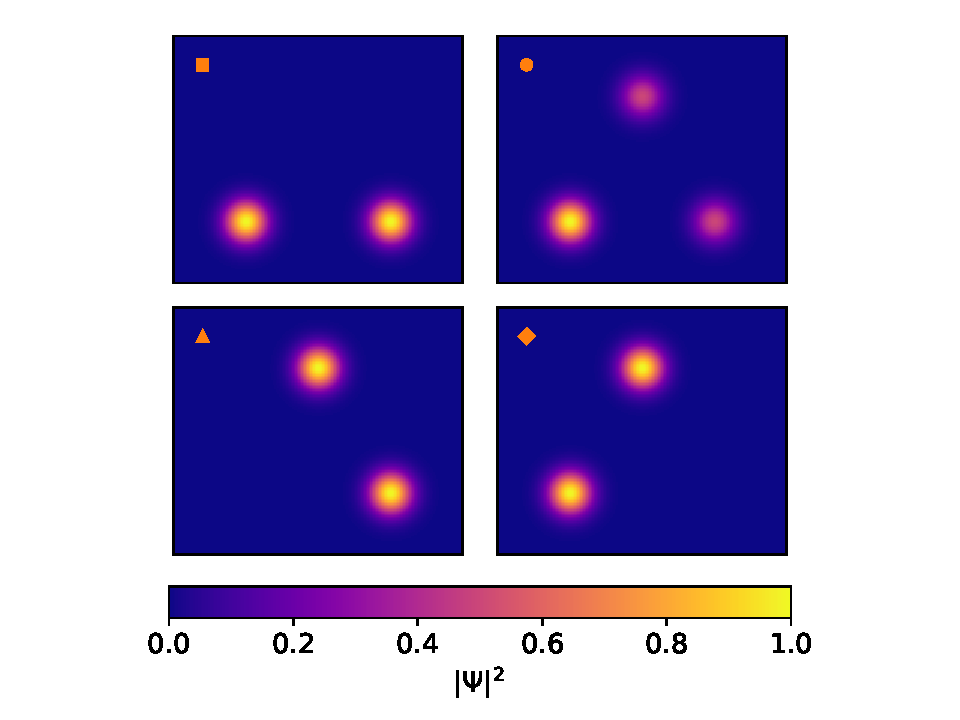
\includegraphics[width=4.2 in]{./figures/3eigvec.pdf}}
	\caption{(a) Evolution of the eigenvalues of the 3-site Kitaev triangle along the closed parameter path for $\phi$ on the three edges. (b) MZM wavefunctions at different points of the parameter path. Clockwise from the upper left panel: $\bm \phi_1 \rightarrow \frac{1}{2}(\bm \phi_1 + \bm \phi_2)\rightarrow \bm \phi_2\rightarrow \bm \phi_3$.}
	\label{fig:3eig}
\end{figure}

Indeed, Fig.~\ref{fig:3eig} shows that the MZM stays at zero energy throughout the parameter path that interchanges their positions. To show that such an operation indeed realizes braiding, we explicitly calculated the many-body Berry phase of the evolution \cite{supp,aliceaNonAbelianStatisticsTopological2011,liManipulatingMajoranaZero2016} and found the two degenerate many-body ground states acquire a $\frac{\pi}{2}$ difference in their Berry phases as expected \cite{aliceaNonAbelianStatisticsTopological2011}. Compared to the minimum T-junction model with four sites \cite{aliceaNonAbelianStatisticsTopological2011}, our Kitaev triangle model only requires three sites to achieve braiding between two MZM, and is potentially also easier to engineer experimentally. In the next section we will show that a more mesoscopic hollow-triangle structure can achieve similar results and may be preferred in other materials platforms.


\section{Hollow Triangles}

For systems with less fine-tuned Hamiltonians than the minimal model in the previous section, it is more instructive to search for MZM based on topological arguments. In this section we show that MZM generally appear at the corners of a hollow triangle, which can be approximated by joining three finite-width chains or ribbons whose bulk topology is individually tuned by the same uniform vector potential.

To this end, we first show that topological phase transitions can be induced by a vector potential in a spinless $p$-wave superconductor ribbon. In comparison with similar previous proposals that mostly focused on vector potentials or supercurrents flowing along the chain \cite{romitoManipulatingMajoranaFermions2012, takasanSupercurrentinducedTopologicalPhase2022}, we consider in particular the tunability by varying the direction of the vector potential relative to the length direction of the ribbon, which will become instrumental in a triangular structure.

Consider Eq.~\eqref{eq:HBdG} on a triangular lattice defined by unit-length lattice vectors $(\mathbf a_1, \mathbf a_2) = (\hat{x}, \frac{1}{2}\hat{x} + \frac{\sqrt{3}}{2}\hat{y})$ with $W$ unit cells along $\mathbf a_2$ but infinite unit cells along $\mathbf a_1$, and assume the Peierls phases are due to a uniform vector potential $\mathbf A$ so that $\phi_{jl} = \mathbf A\cdot \mathbf r_{jl}$. We also introduce $\mathbf a_3 \equiv -\mathbf a_1 + \mathbf a_2$ for later convenience. The Hamiltonian is periodic along $x$ and can be Fourier transformed through $\cc_{m,n} = \dfrac{1}{\sqrt{N}} \sum_{k} \cc_{k,n} e^{-i km}$, where $m,n$ label the lattice sites as $\mathbf r_{m,n} = m\mathbf a_1 + n \mathbf a_2$. The resulting momentum space Hamiltonian can be written as the following block form up to a constant
\begin{eqnarray}\label{eq:Hribbon}
      \ham &=& \dfrac{1}{2} \sum_k \Psi_k^\dagger \left(
    \begin{matrix}
      h_t(k) & h_\Delta(k) \\
      h_\Delta^\dagger(k) & -h_t^*(-k)
    \end{matrix} \right)
    \Psi_k \\\nonumber
&\equiv&\dfrac{1}{2} \sum_k \Psi_k^\dagger H(k)
    \Psi_k
\end{eqnarray}
where $\Psi_k \equiv (c_{k,1},\dots, c_{k,W},c^\dag_{-k,1},\dots c_{-k,W}^\dag)^T$. $h_t(k)$ is a $W\times W$ Hermitian tridiagonal matrix with $(h_t)_{n,n} = -2t\cos(k+\mathbf A\cdot \mathbf a_1) - \mu$ and $(h_t)_{n,n+1} = -t\left( e^{i(-k+\mathbf A\cdot \mathbf a_3)}  + e^{i\mathbf A \cdot \mathbf a_2}\right)$. $h_\Delta(k)$ is a $W\times W$ tridiagonal matrix with $(h_\Delta)_{n,n} = -2i\de \sin k $ and $(h_\Delta)_{n,n\pm 1} = \mp \de\left[ e^{-i(\pm k + \frac{2\pi}{3})} + e^{-i\frac{\pi}{3}} \right]$.

By transforming Eq.~\eqref{eq:Hribbon} to the Majorana basis using the unitary transformation:
\begin{eqnarray}
    U\equiv \dfrac{1}{\sqrt{2}} \left(
  \begin{matrix}
    1 & 1 \\
    -i & i
  \end{matrix} \right) \otimes \mathbb{I}
\end{eqnarray}
where $\mathbb{I}$ is a ${W\times W}$ identity matrix, and defining $A_k\equiv -iU H(k) U^\dag$, not to be confused with the vector potential, one can calculate the Majorana number \cite{kitaevUnpairedMajoranaFermions2001} $\mathcal{M}$ of the 1D ribbon as \cite{liTopologicalSuperconductivityInduced2014}
\begin{eqnarray}
\mathcal{M} = {\rm sgn}\left[{{\rm Pf}(A_{k=0}) {\rm Pf}(A_{k=\pi})}\right]
\end{eqnarray}
where $\text{Pf}$ stands for the Pfaffian of a skew-symmetric matrix \cite{kitaevUnpairedMajoranaFermions2001}. When $\mathcal{M} = -1$, the 1D system is in a nontrivial topological phase with MZM appearing at open ends of semi-infinite ribbons, and otherwise for $\mathcal{M} = 1$.

\begin{figure}[!ht]
  \hspace{12pt}
  \subfloat[]{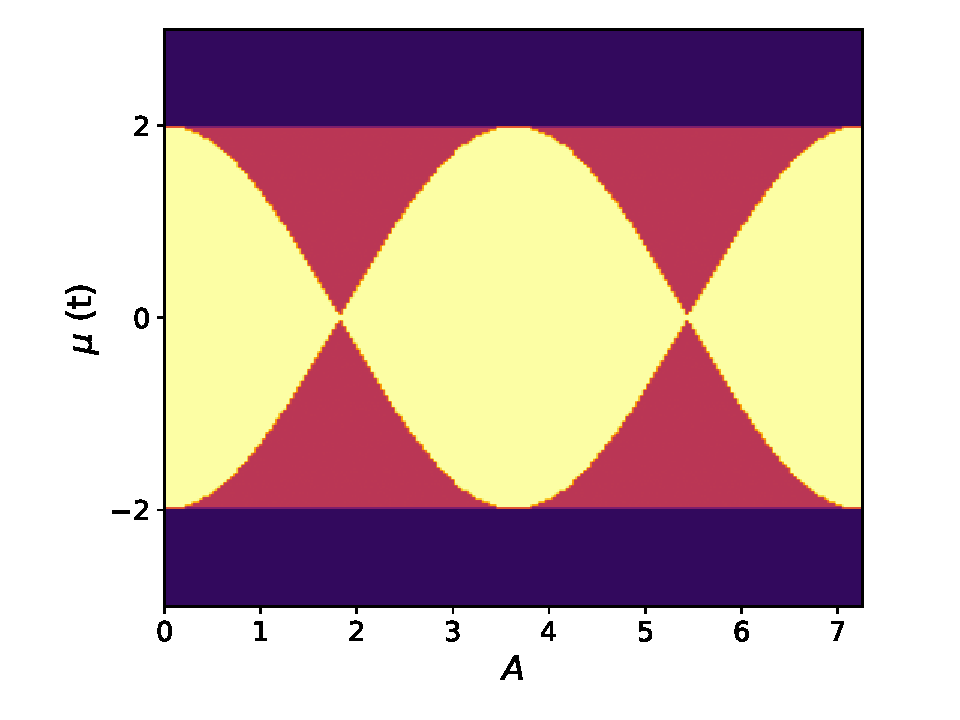
\includegraphics[width=0.532\textwidth]{./figures/topological-phase-diagram-1pi6-n-1.pdf}} \\
  \vspace{-15pt}
  \subfloat[]{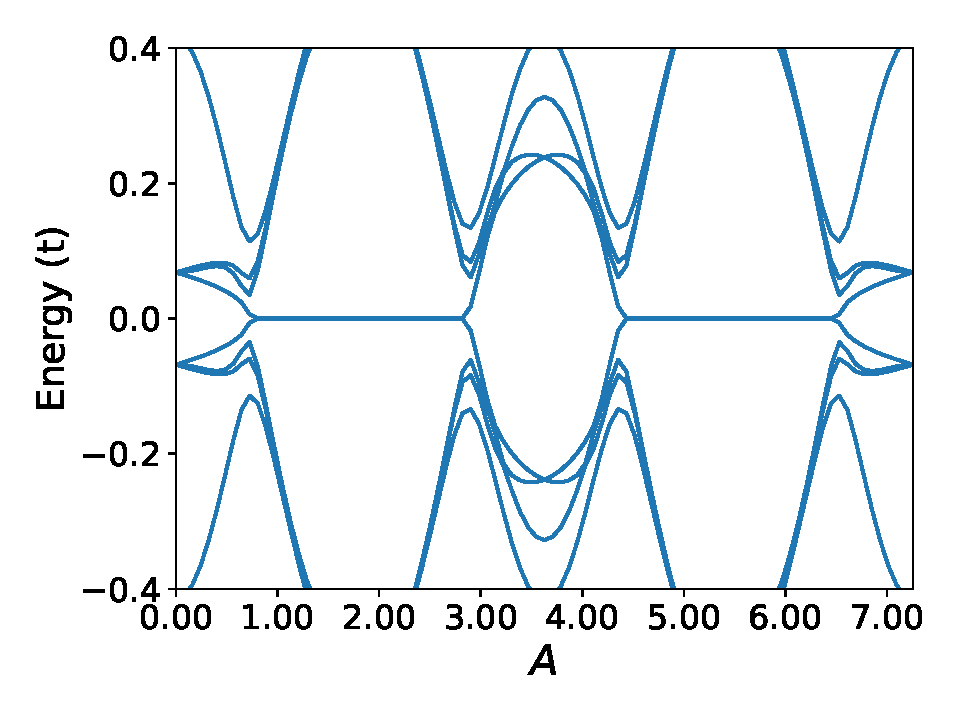
\includegraphics[width=0.50\textwidth]{./figures/spectral-flow-nr-50-w-1-mu-1_6.pdf}}
\caption{(a) Topological phase diagram for a $W=1$ triangular chain with the Hamiltonian Eq.~\eqref{eq:Hribbon} obtained by superimposing the $\mathcal{M}(A, \mu)$ plots of 1D chains with $\mathbf A = A\hat{y}$ and $\mathbf A = A(\frac{\sqrt{3}}{2}\hat{x}+\frac{1}{2}\hat{y})$. Color scheme: white---$\mathcal{M}=1$, dark blue---$\mathcal{M}=-1$, light blue---$\mathcal{M}=0$ (b) Near-gap BdG eigen-energies vs $A$ for a finite triangle with edge length $L = 50$, $W=1$, and $\mu=1.6$.}
  \label{fig: pd}
\end{figure}

In Fig.~\ref{fig: pd} (a) we show the topological phase diagrams for a 1D ribbon with width $W=1$, $\mathbf A = A\hat{y}$ and $\mathbf A = A(\frac{\sqrt{3}}{2}\hat{x}+\frac{1}{2}\hat{y})$ superimposed (see below). We found that the vector potential component normal to the ribbon length direction has no effect on the Majorana number, nor does the sign of its component along the ribbon length direction. However, topological phase transitions can be induced by varying the size of the vector potential component along the ribbon, consistent with previous results \cite{romitoManipulatingMajoranaFermions2012, takasanSupercurrentinducedTopologicalPhase2022}. These properties motivate us to consider the structure of a hollow triangle formed by three finite-width ribbons subject to a uniform vector potential $\mathbf A = A\hat{y}$ as illustrated in Fig.~\ref{fig:triangles} (b). The light blue color on the phase diagram Fig.~\ref{fig: pd} (a) therefore means that the bottom edge and the two upper edges of the hollow triangle have different $\mathcal{M}$, which should give rise to MZM localized at the two bottom corners if the triangle is large enough so that bulk-edge correspondence holds, and gap closing does not occur at other places along its edges.

To show that corner MZM indeed appear when the conditions given by the phase diagram Fig.~\ref{fig: pd} (a) are met, we directly diagonalize the BdG Hamiltonian of a finite hollow triangle with edge length $L=50$ and width $W=1$. Fig.~\ref{fig: pd} (b) shows the spectral flow (BdG eigen-energies evolving with increasing vector potential $A$) close to zero energy at chemical potential $\mu=1.6$. Indeed, zero-energy modes appear in the regions of $\mu$ and $A$ consistent with the phase diagram (except when the bulk band gap is too small; see \cite{supp} for some examples.). Hollow triangles with larger larger $W$ also have qualitatively similar behavior, although the phase diagrams are more complex \cite{supp}. The eigenfunctions for the zero-energy modes at $A=2.75$ and $\mu=1.6$ in Fig.~\ref{fig: rotation} (b) also confirm their spatial localization at the bottom corners of the triangle.

\begin{figure*}[!ht]
  \subfloat[]{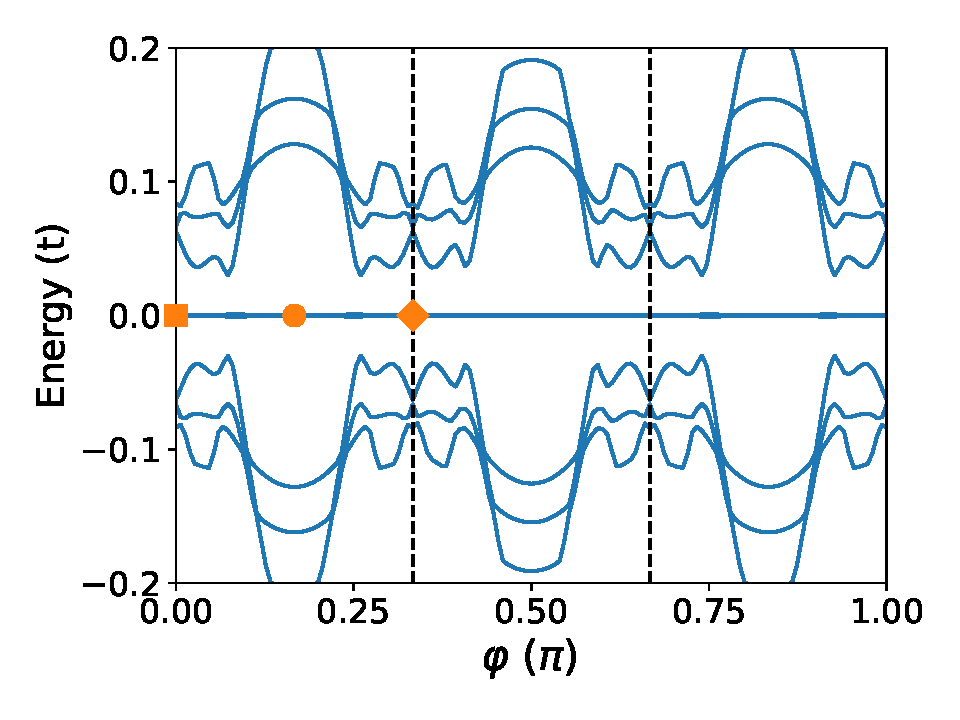
\includegraphics[height=150pt]{./figures/spectral-flow-rotation-constant-vector-nr-50-w-1-mu-1_6.pdf}} \\
  \subfloat[]{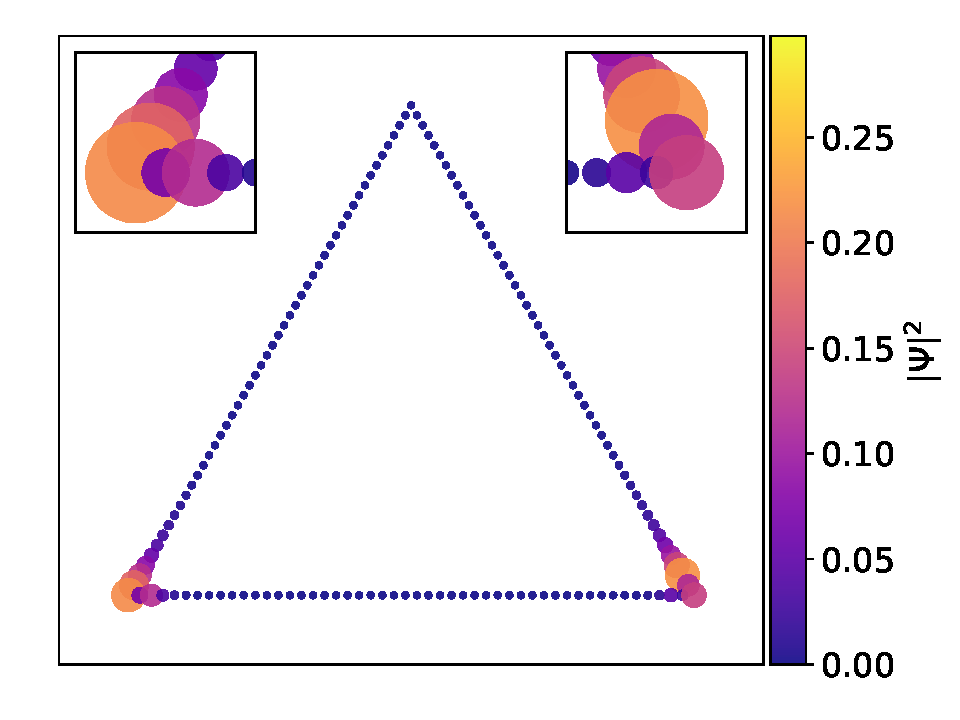
\includegraphics[height=125pt]{./figures/GS-T-Square.pdf}}
  \hspace{-20pt}
  \subfloat[]{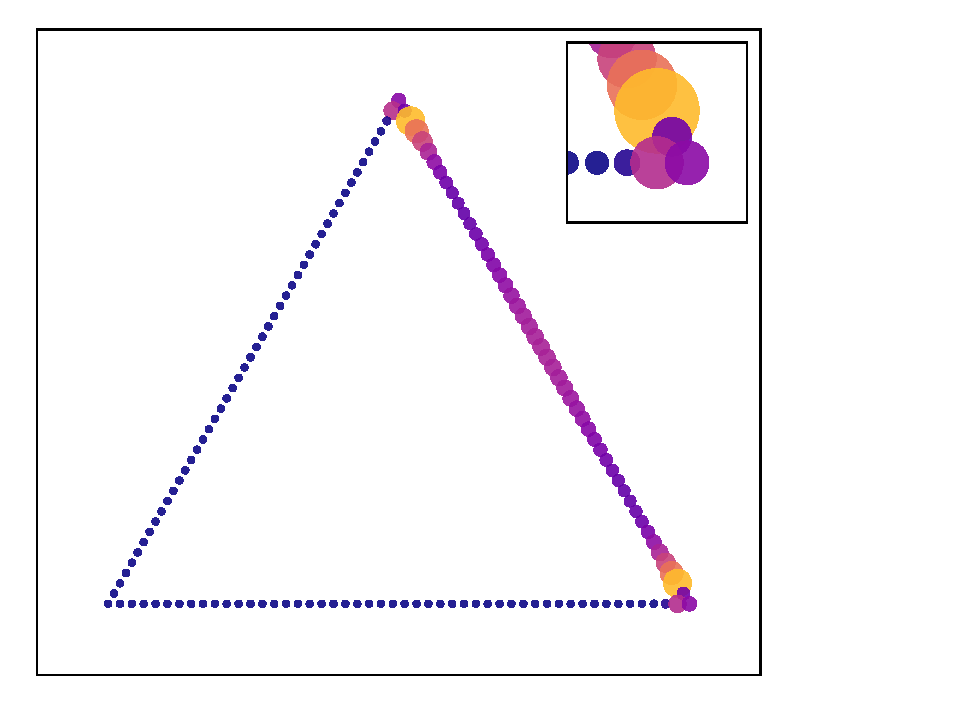
\includegraphics[height=125pt]{./figures/GS-T-Circle.pdf}}
  \hspace{-24pt}
  \subfloat[]{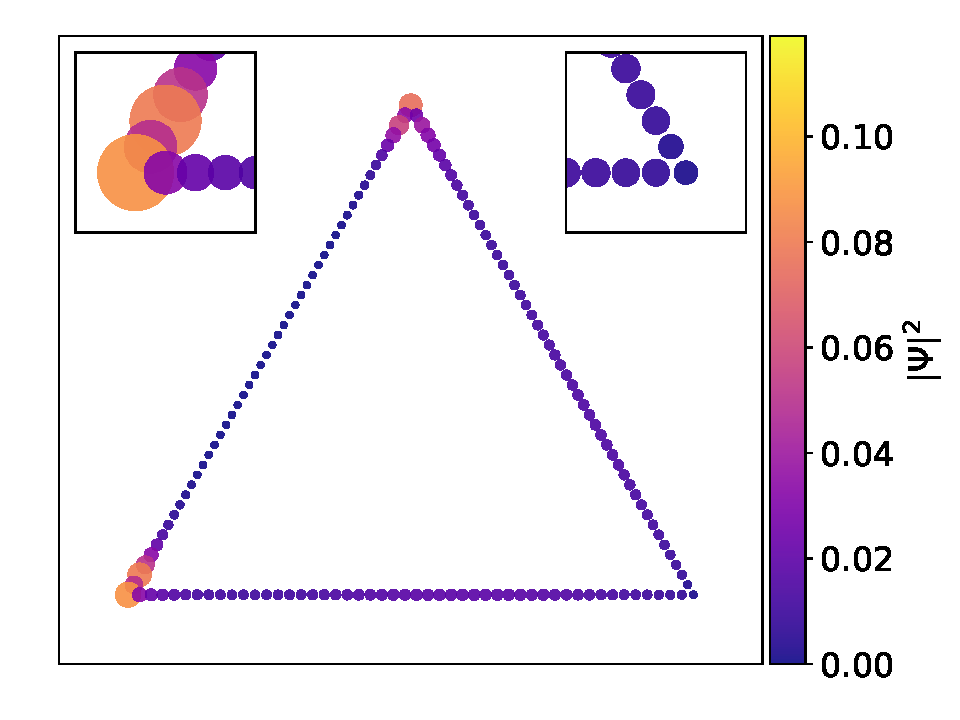
\includegraphics[height=127pt]{./figures/GS-T-Diamond.pdf}}
  \caption{(a) Spectral flow of a hollow triangle with $W=1$, $L=50$, $\mu=1.6$, and $A=2.75$ with increasing rotation angle $\varphi$, defined through $\mathbf A = A(-\sin\varphi \hat{x} + \cos\varphi \hat{y})$. (b-d) BdG eigenfunction $|\Psi|^2$ summed over the two zero modes at $\varphi = 0, \frac{\pi}{6}$, and $\frac{\pi}{3}$, respectively.}
  \label{fig: rotation}
\end{figure*}

We finally show that rotating the uniform vector potential in-plane can manipulate the positions of the MZM without hybridizing them with bulk states for certain ranges of $\mu$ and $A$. Fig.~\ref{fig: rotation} (a) plots the spectral flow versus the in-plane azimuthal angle of $\mathbf A$, which clearly shows that the zero-energy modes persist throughout the rotation and the bulk gap never closes. Figs.~\ref{fig: rotation} (b-d) plot the BdG wavefunctions of the MZM at special values of $\varphi$. One can see that the two MZM appear to cycle through the three vertices by following the rotation of $\mathbf A$. The robustness of the MZM therefore requires the condition of two edges being in a different topological phase from the third one to be satisfied throughout the rotation. Such a criterion combined with the individual phase diagrams of the edges can help isolate the desired parameter regions of $\mu$ and $A$. We also note that the positions of the MZM do not interchange after $\varphi$ increases from 0 to $\pi$, different from the situation of the minimal Kitaev triangle in Fig.~\ref{fig:3eig}. The reason is that the MZM in the latter case are not due to bulk-boundary correspondence [the values of $A = \frac{2\pi}{3\sqrt{3}}$ and $\mu=0$ are a critical point in the phase diagram Fig.~\ref{fig: pd} (a)]. While the positions of the MZM at special points along the parameter path in the hollow triangle case have to be additionally constrained by the bulk topological phases of the three edges, that for the Kitaev triangle have more flexibility and are also protected by the finite size of the system.



\begin{figure}[!ht]
  \hspace{28pt}
  \subfloat[]{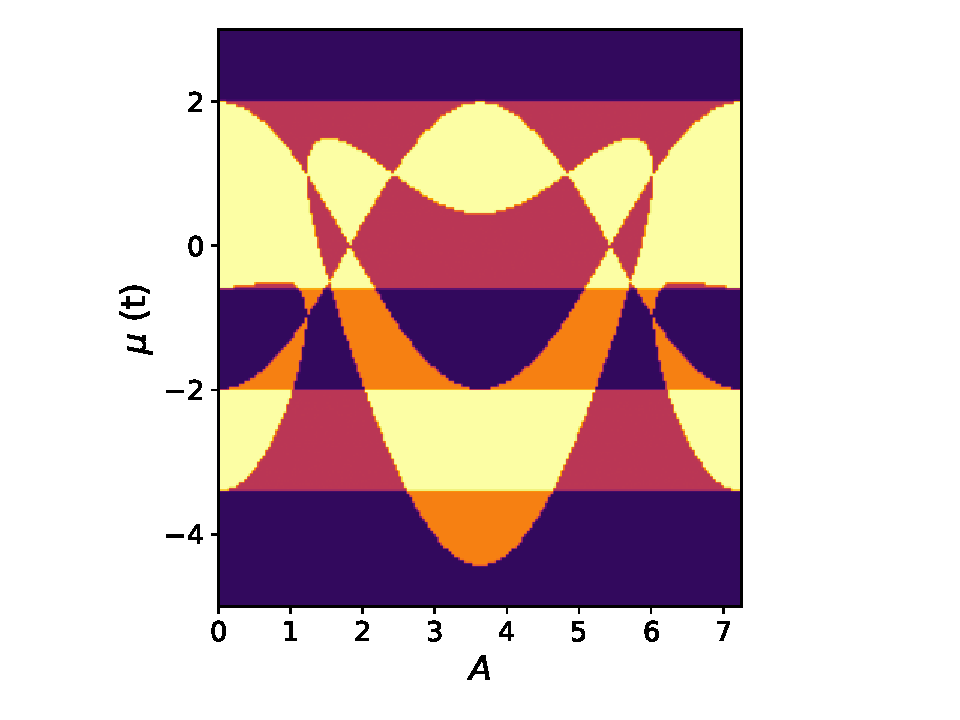
\includegraphics[width=0.50\textwidth]{./figures/supp/topological-phase-diagram-1pi6-n-3.pdf}}
  \hspace{-40pt}
  \subfloat[]{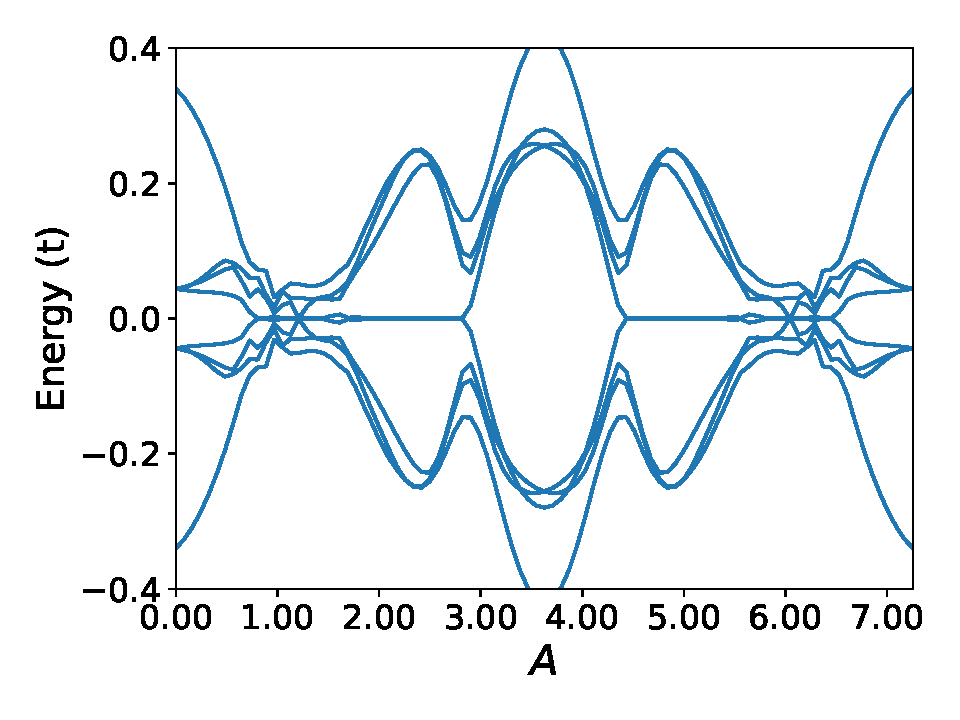
\includegraphics[width=0.50\textwidth]{./figures/supp/spectral-flow-nr-50-w-3-mu-1_6.pdf}} \\
  \hspace{70pt}
  \subfloat[]{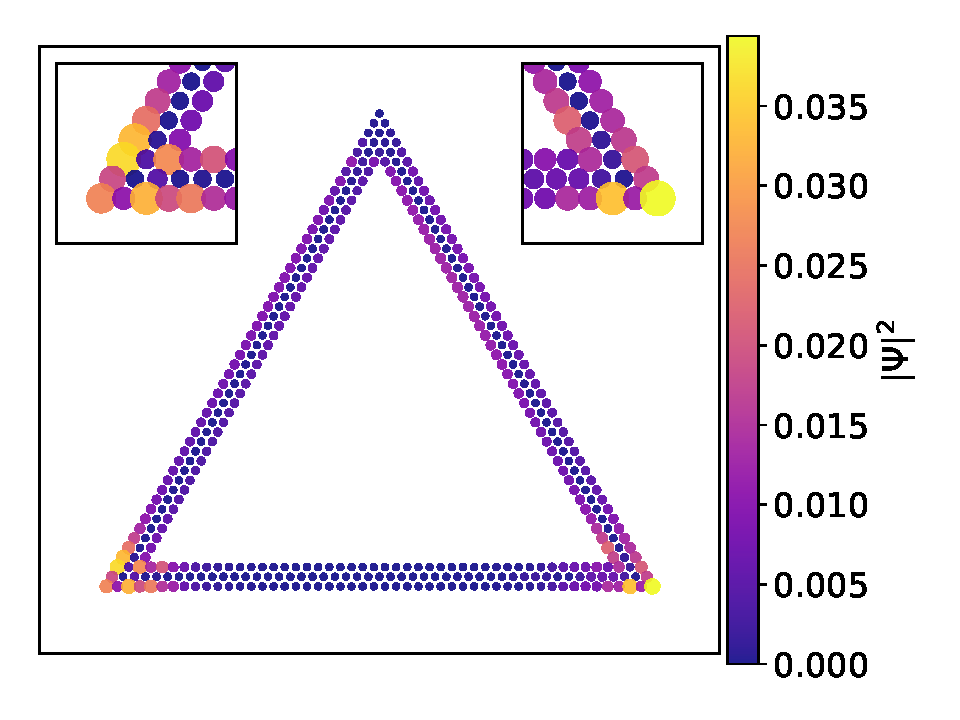
\includegraphics[width=0.50\textwidth]{./figures/supp/GS-A-2_74-nr-50-w-3-mu-1_6.pdf}}
  \caption{(a) Topological phase diagram for a $W=3$ hollow triangle obtained by overlapping the $\mathcal{M}(A, \mu)$ plots of 1D chains with $\mathbf A = A\hat{y}$ and $\mathbf A = A(\frac{\sqrt{      3}}{2}\hat{x}+\frac{1}{2}\hat{y})$. Color scheme: white---$\mathcal{M}=1$, dark blue---$\mathcal{M}=-1$, light blue---$\mathcal{M}=0$ (b) Near-gap BdG eigen-energies vs $A$ for a finite triangle with edge length $L=50$, $W=3$, and $\mu=1.6$. (c) BdG eigenfunction $|\Psi|^2$ summed over the two zero modes at $A=2.4709$.}
  \label{fig: supp pd}
\end{figure}

A model that is closer to a realistic hollow triangular island is the finite-width triangular chain or ribbon. An example, illustrated in Figure \ref{fig: supp pd} (c), has its edge length $L=50$ and width $W=3$. The phase diagram Fig.~\ref{fig: supp pd} (a) is created in a similar way as that in Fig. \ref{fig: pd} (a), assuming a constant vector potential and infinitely long $W=3$ ribbons. The spectral flow for the actual triangle with $\mu = 1.6$ in Fig.~\ref{fig: supp pd} (b) shows MZM in the parameter regions in agreement with the phase diagram. Fig.~\ref{fig: supp pd} (c) plots the MZM wavefunction for $A=2.7409$ and $\mu=1.6$ that are indeed well localized at the bottom corners.

\begin{figure}[!ht]
  \hspace{-20pt}
  \subfloat[]{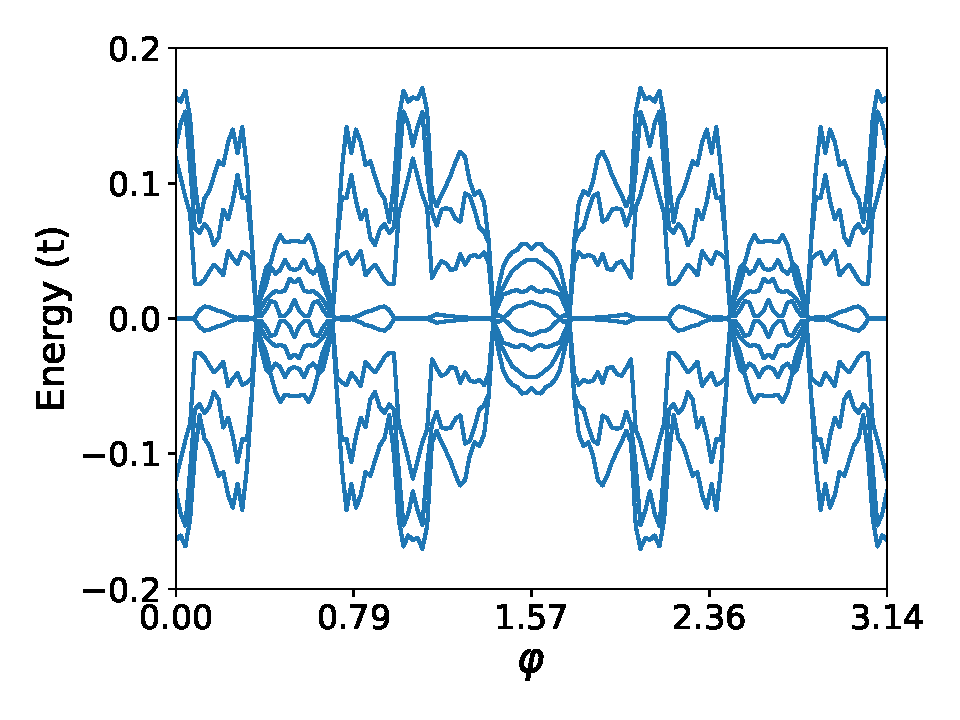
\includegraphics[width=0.5\textwidth]{./figures/supp/spectral-flow-w-3.pdf}}\\
  \subfloat[]{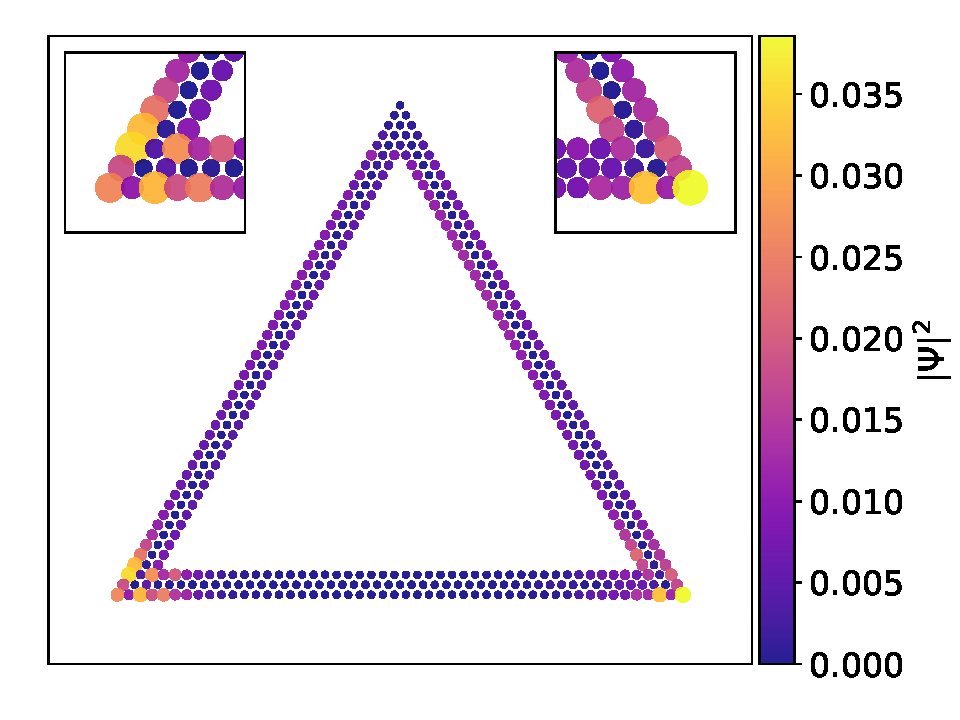
\includegraphics[width=0.4\textwidth]{./figures/supp/GS-T-Square-w-3.pdf}}
  %\subfloat[]{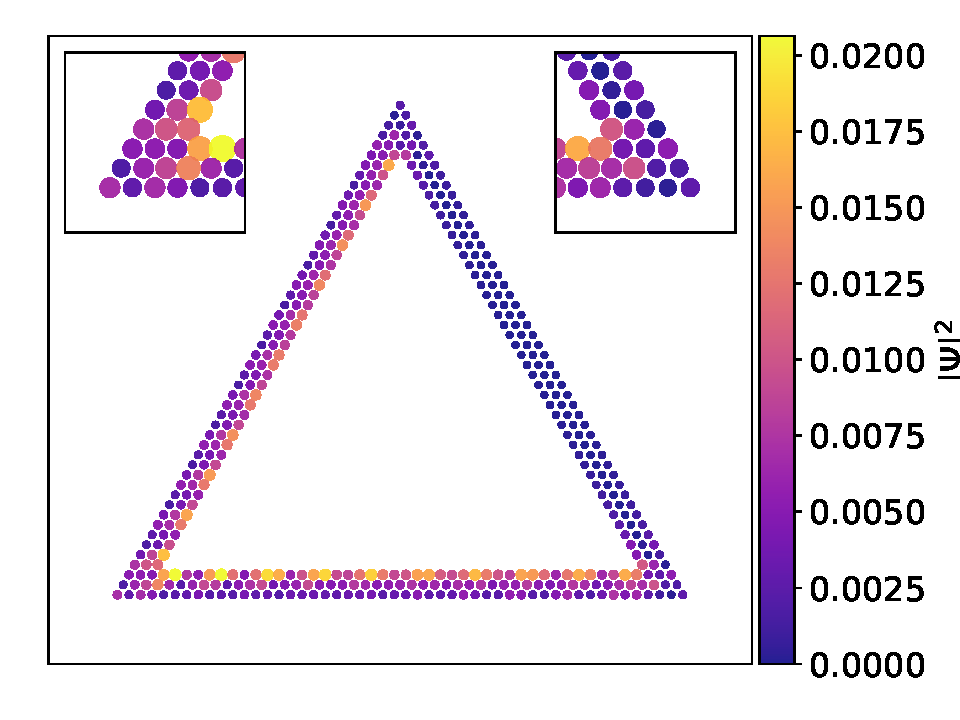
\includegraphics[width=0.4\textwidth]{./figures/supp/GS-T-Circle-w-3.pdf}}
  \subfloat[]{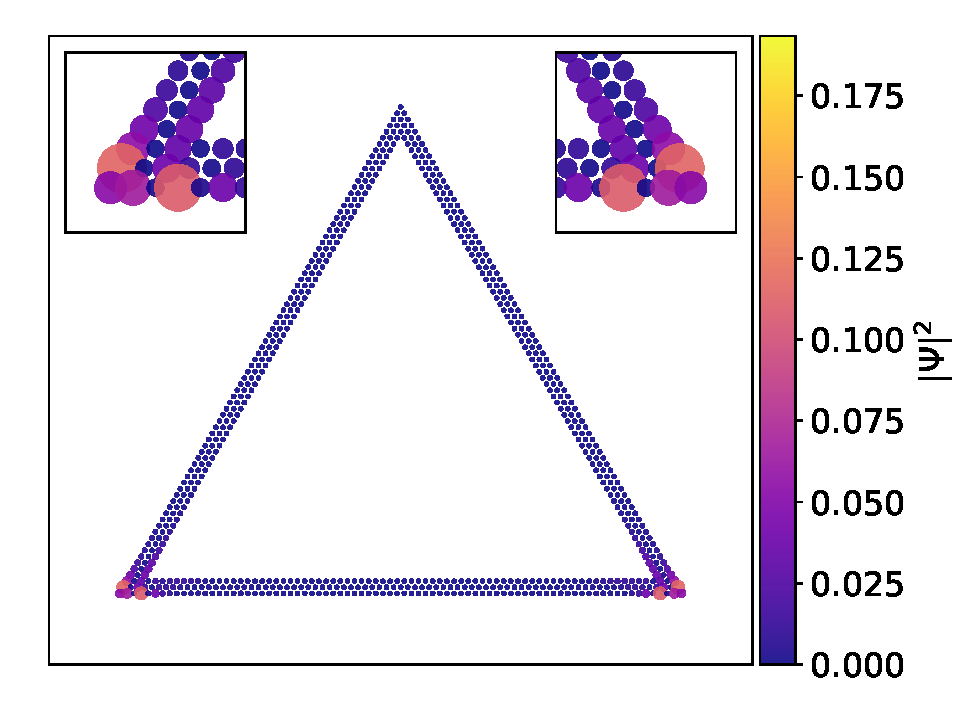
\includegraphics[width=0.4\textwidth]{./figures/supp/GS-T-Diamond-w-3.pdf}}
  \caption{(a) Spectral flow of a hollow triangle with $W=3$, $L=50$, $\mu=1.6$, and $A=2.75$ with increasing rotation angle $\varphi$, defined through $\mathbf A = A(-\sin\varphi \hat{x} + \cos\varphi \hat{y})$. (b-c) BdG eigenfunction $|\Psi|^2$ summed over the two zero modes at $\varphi = 0$ and $\frac{\pi}{3}$, respectively.}
  \label{fig: supp rotation}
\end{figure}

We next rotate the uniform vector potential to examine how the MZM move on a hollow triangle. Figure~\ref{fig: supp rotation} shows the spectral flow and eigenfunctions as we rotate $\varphi=0$ to $\varphi=\pi$ counterclockwisely. The two MZM cycle through the three vertices in a similar manner as that in Fig.~4 of the main text (only the MZM wavefunctions at $\varphi = 0$ and $\frac{\pi}{3}$ are plotted as representatives of the $\varphi = n\pi/3$ cases). Note that the spectral flow has 3-fold rotation symmetry but not 6-fold, since increasing $\varphi$ by $\frac{2\pi}{3}$ is equivalent to rotating the coordinate system clockwisely by $\frac{2\pi}{3}$. In contrast, rotating the vector potential by $\frac{\pi}{3}$, if without an additional sign change of the $p$-wave pairing potential, is not an exact symmetry of the finite triangle. Also we did not try to scrutinize the phase diagram to find a parameter path in which the bulk gap does not close, as in the $W=1$ case in the main text. Here we just point out that identifying a system-specific parameter path for adiabatic manipulation of MZM is in principle always possible, especially if one is allowed to have more knobs other than $\varphi$ in real structures, such as tuning the chemical potential of individual edges or the size of the vector potential, etc.

\section{Braiding MZM in a small network of triangles}

\begin{figure}[!ht]
  \hspace{-30pt}
  \subfloat[]{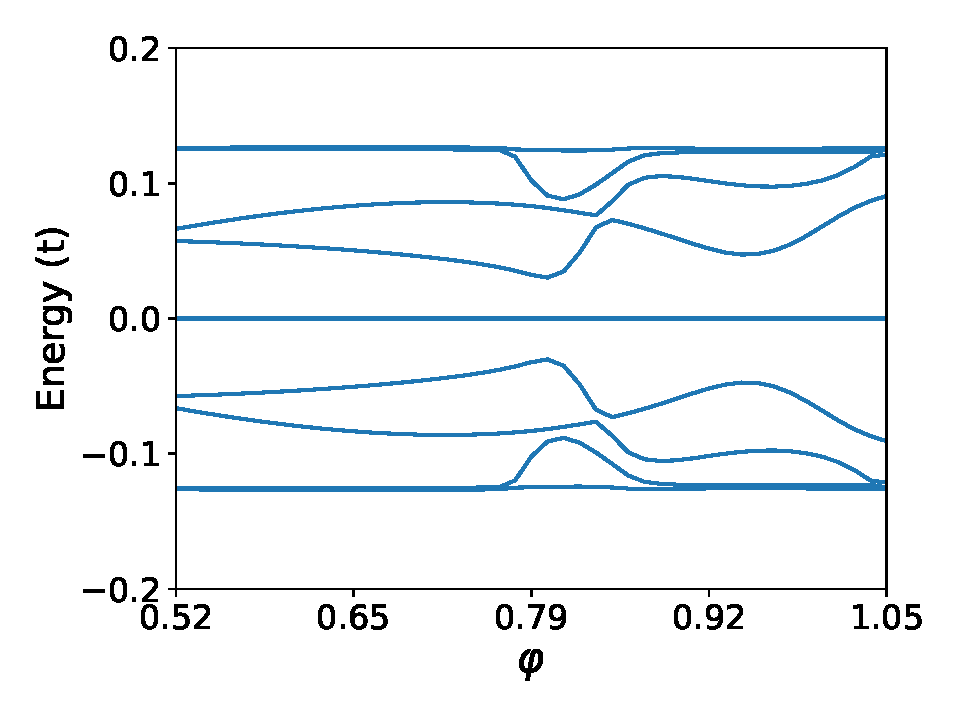
\includegraphics[width=0.4\textwidth]{./figures/supp/spectral-flow-braiding.pdf}} \\
  \vspace{-10pt}
  \subfloat[]{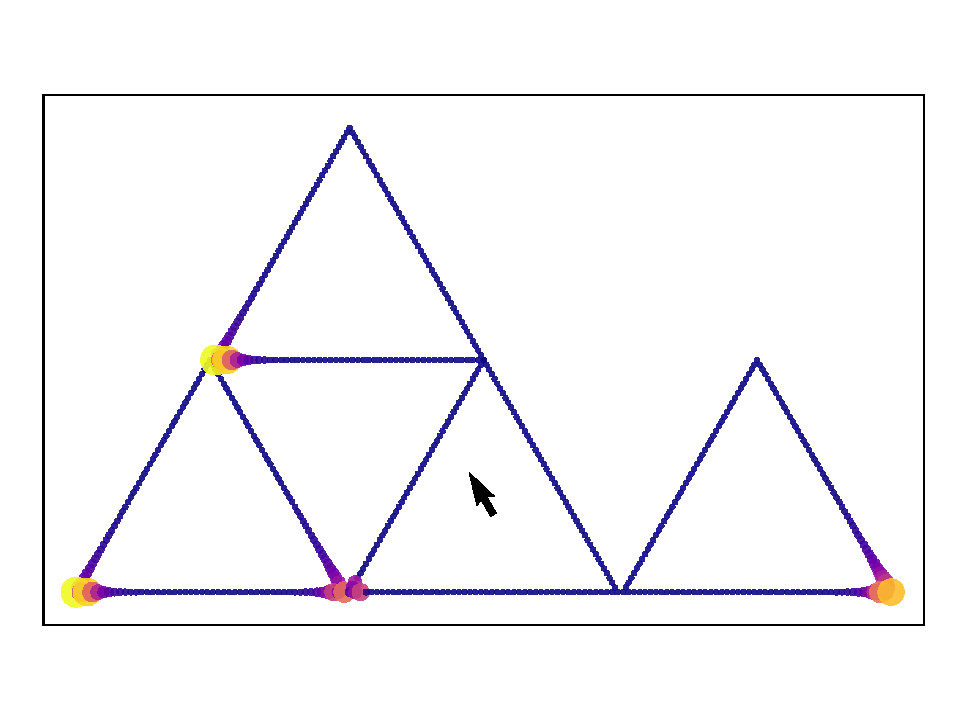
\includegraphics[width=0.30\textwidth]{./figures/supp/GS-T-0_5236.pdf}}
  \subfloat[]{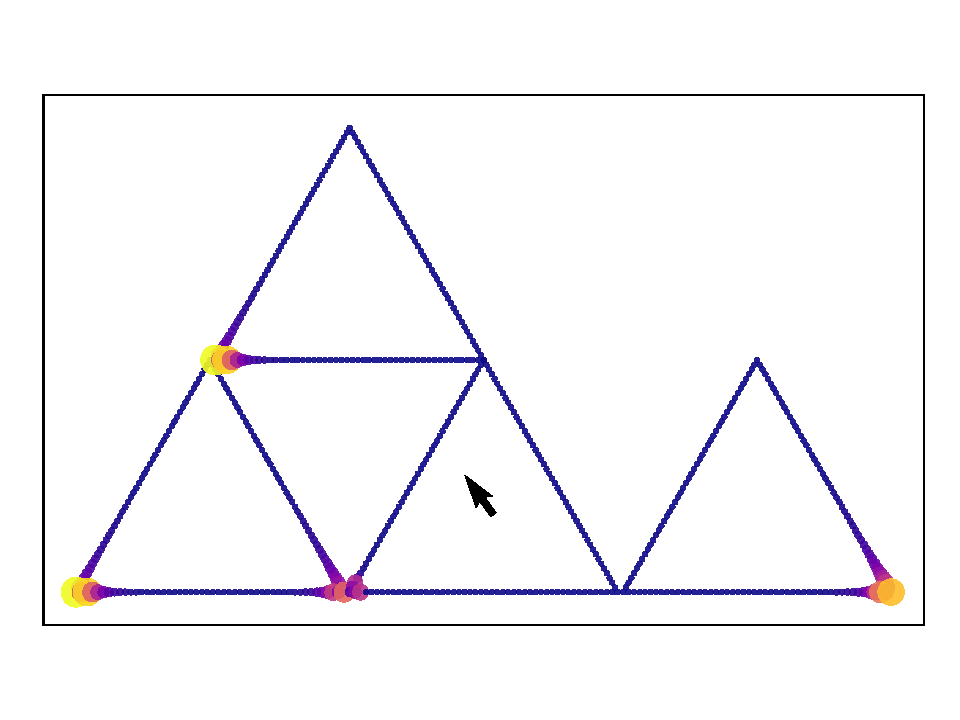
\includegraphics[width=0.30\textwidth]{./figures/supp/GS-T-0_6283.pdf}}
  \subfloat[]{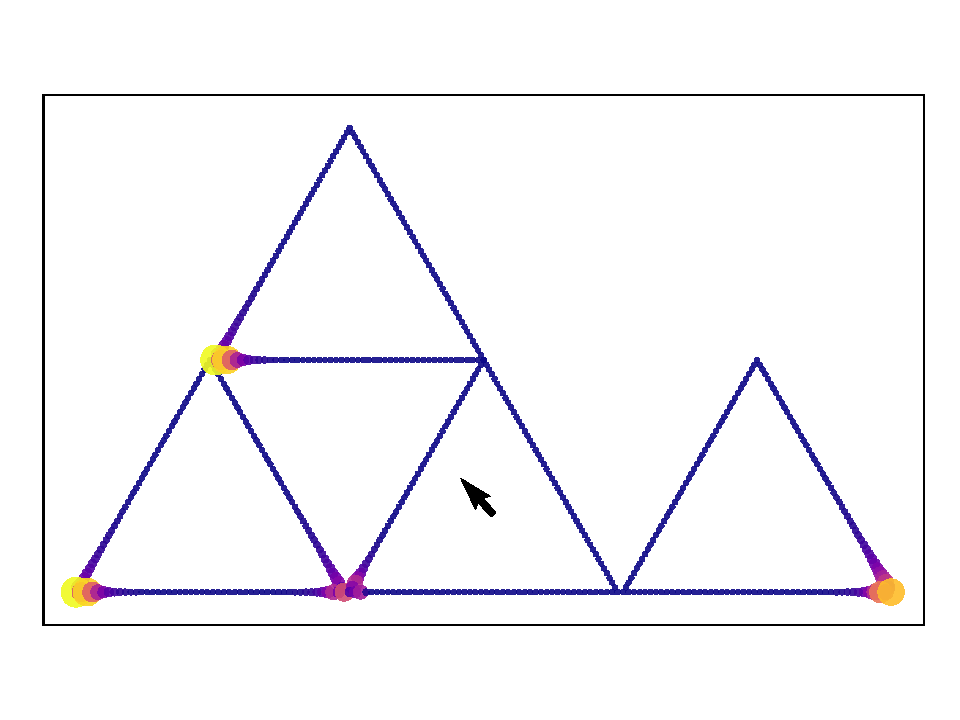
\includegraphics[width=0.30\textwidth]{./figures/supp/GS-T-0_7330.pdf}} \\
  \subfloat[]{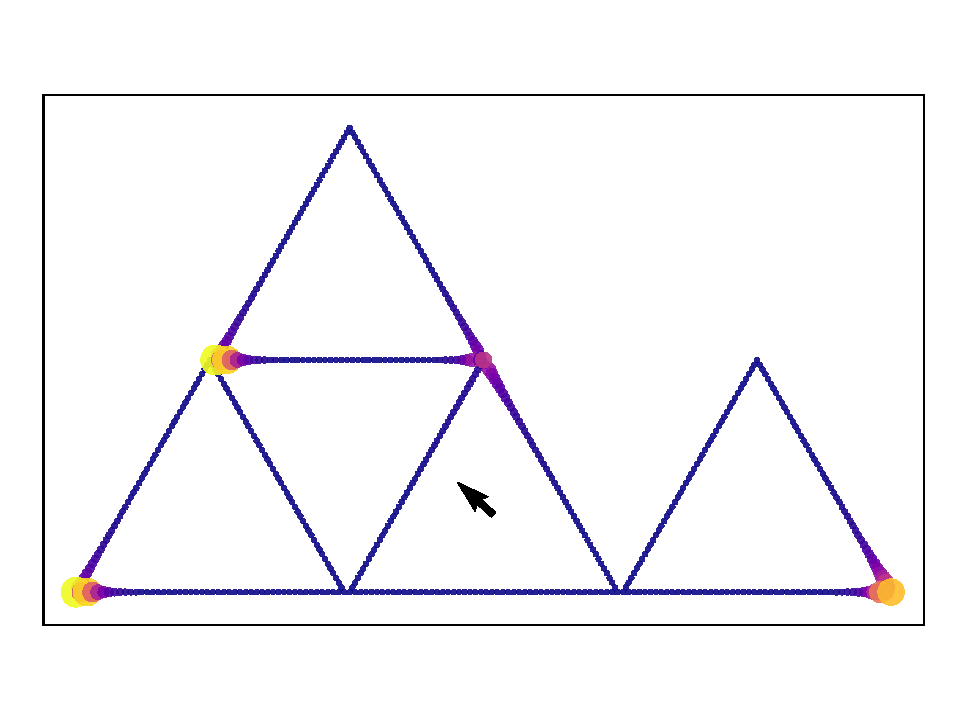
\includegraphics[width=0.30\textwidth]{./figures/supp/GS-T-0_8378.pdf}}
  \vspace{-10pt}
  \subfloat[]{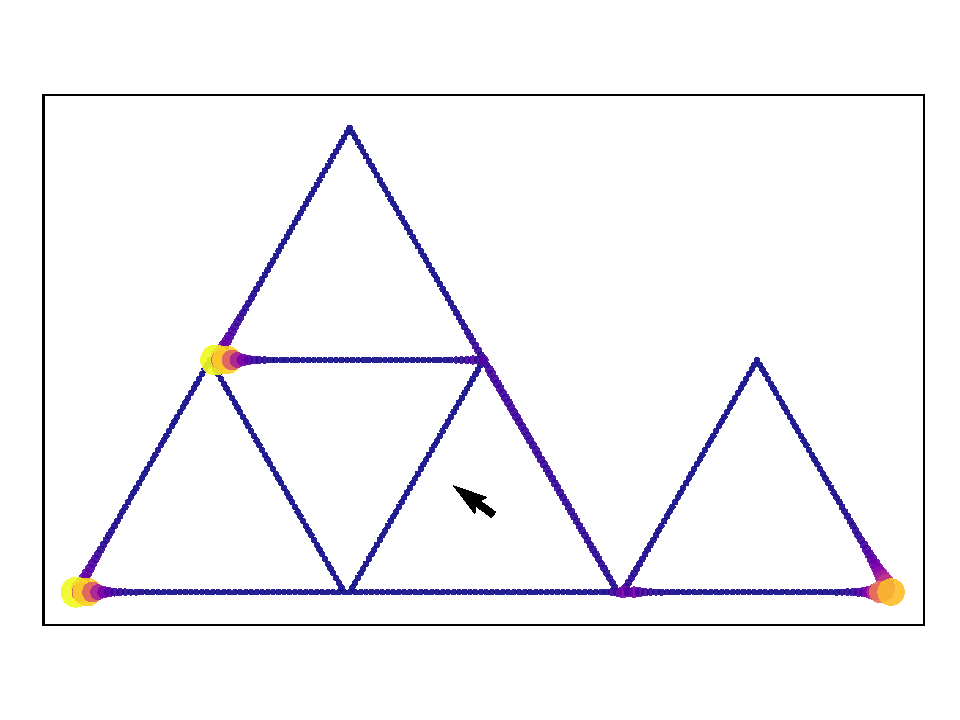
\includegraphics[width=0.30\textwidth]{./figures/supp/GS-T-0_9425.pdf}}
  \subfloat[]{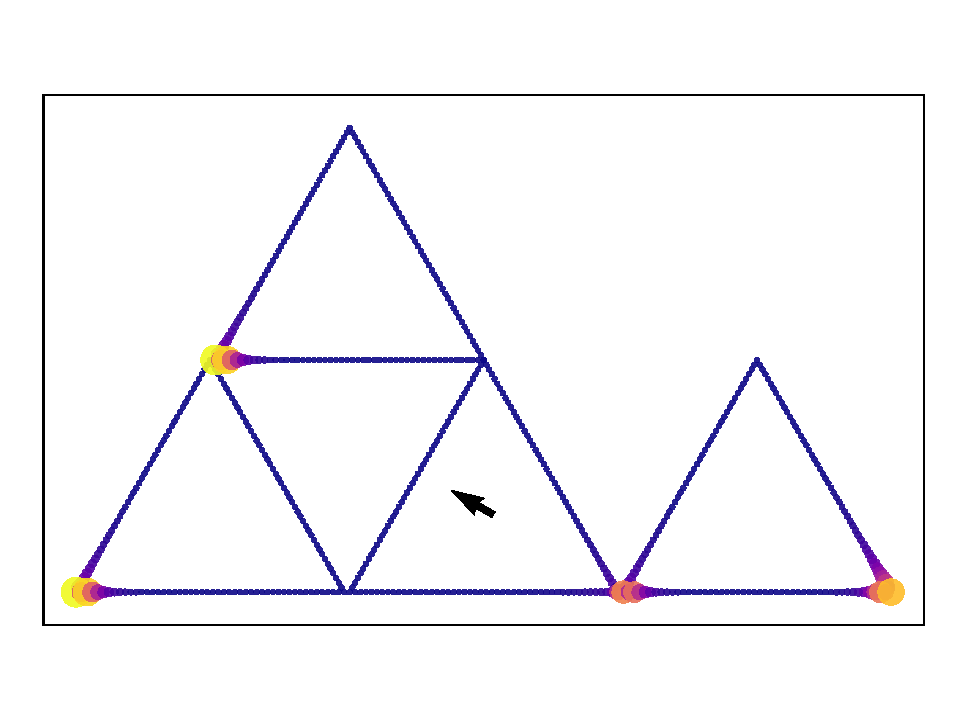
\includegraphics[width=0.30\textwidth]{./figures/supp/GS-T-1_0472.pdf}}
  \caption{(a) Spectral flow for the critical step of swapping $\gamma_2$ and $\gamma_3$ in the example of Fig.~5 in the main text, calculated using four corner-sharing triangles of $W=1$ and $L=50$, with $\mu=1.6$ and $A=2.6$. Vector potential for the middle triangle in the bottom row can rotate according to $\mathbf A = A(-\sin\varphi \hat{x} + \cos\varphi \hat{y})$ from $\varphi = \frac{\pi}{6}$ to $\frac{\pi}{3}$, while the other three have fixed $\varphi = 0$. (b)-(g) BdG eigenfunction $|\Psi|^2$ summed over the four zero modes at equally-spaced points along the rotation path. The black arrow indicates the direction of the vector potential for the bottom middle triangle.}\label{fig: supp braiding}
\end{figure}

In this section we show that one can braid two out of four MZM, a minimal setting for nontrivial manipulation of the degenerate many-body ground states, by using a small network of corner-sharing triangles. We focus on the critical step of swapping $\gamma_2$ and $\gamma_3$ as labeled in Fig.~5 of the main text. This can be done by rotating the vector potential of the triangle in the middle of the bottom row from $\varphi = \frac{\pi}{6}$ to $\frac{\pi}{3}$. More specifically, when $\varphi = \frac{\pi}{6}$, with the chosen values of $\mu$ and $A$, only the right edge of the said triangle is topologically nontrivial. The chain that hosts $\gamma_{3,4}$ thus extends through this nontrivial edge to the top triangle as in Fig.~\ref{fig: supp braiding} (b). On the other hand, when $\varphi$ increases to $\frac{\pi}{3}$, the nontrivial edge of the middle triangle changes from right to left, which leads to $\gamma_2$ hopping from its left corner to the right through the top corner, while $\gamma_3$ is unaffected [Figs.~\ref{fig: supp braiding} (c-g)]. As a result the $\gamma_2,\gamma_3$ swapping is done without closing the bulk gap, as can be seen from the spectral flow in Fig.~\ref{fig: supp braiding} (a).


\section{Discussion}

The hollow interior of the triangles considered in this work is needed for two reasons: (1) $W\ll L$ is required for bulk-edge correspondence based on 1D topology to hold; (2) A finite $W$ is needed to gap out the chiral edge states of a 2D spinless $p$-wave superconductor based on which Eq.~\eqref{eq:Hribbon} is written. The latter is not essential if one does not start with a spinless $p$-wave supercondutor but a more realistic model such as the Rashba+Zeeman+$s$-wave pairing model. On the other hand, the former constraint may also be removed if one uses the Kitaev triangle. Nonetheless, an effective 3-site Kitaev triangle may emerge as the effective theory of triangular structures if a three-orbital low-energy Wannier basis can be isolated, similar to the continuum theory of moir\'{e} structures. We also note in passing that the corner MZM in our triangles appear due to different reasons from that in higher-order topological superconductors \cite{wangEvidenceMajoranaBound2018,pahomiBraidingMajoranaCorner2020}.

\begin{figure}[!hb]
  \begin{tikzpicture}
    \node[inner sep=0pt] (figure) at (0,0)
    {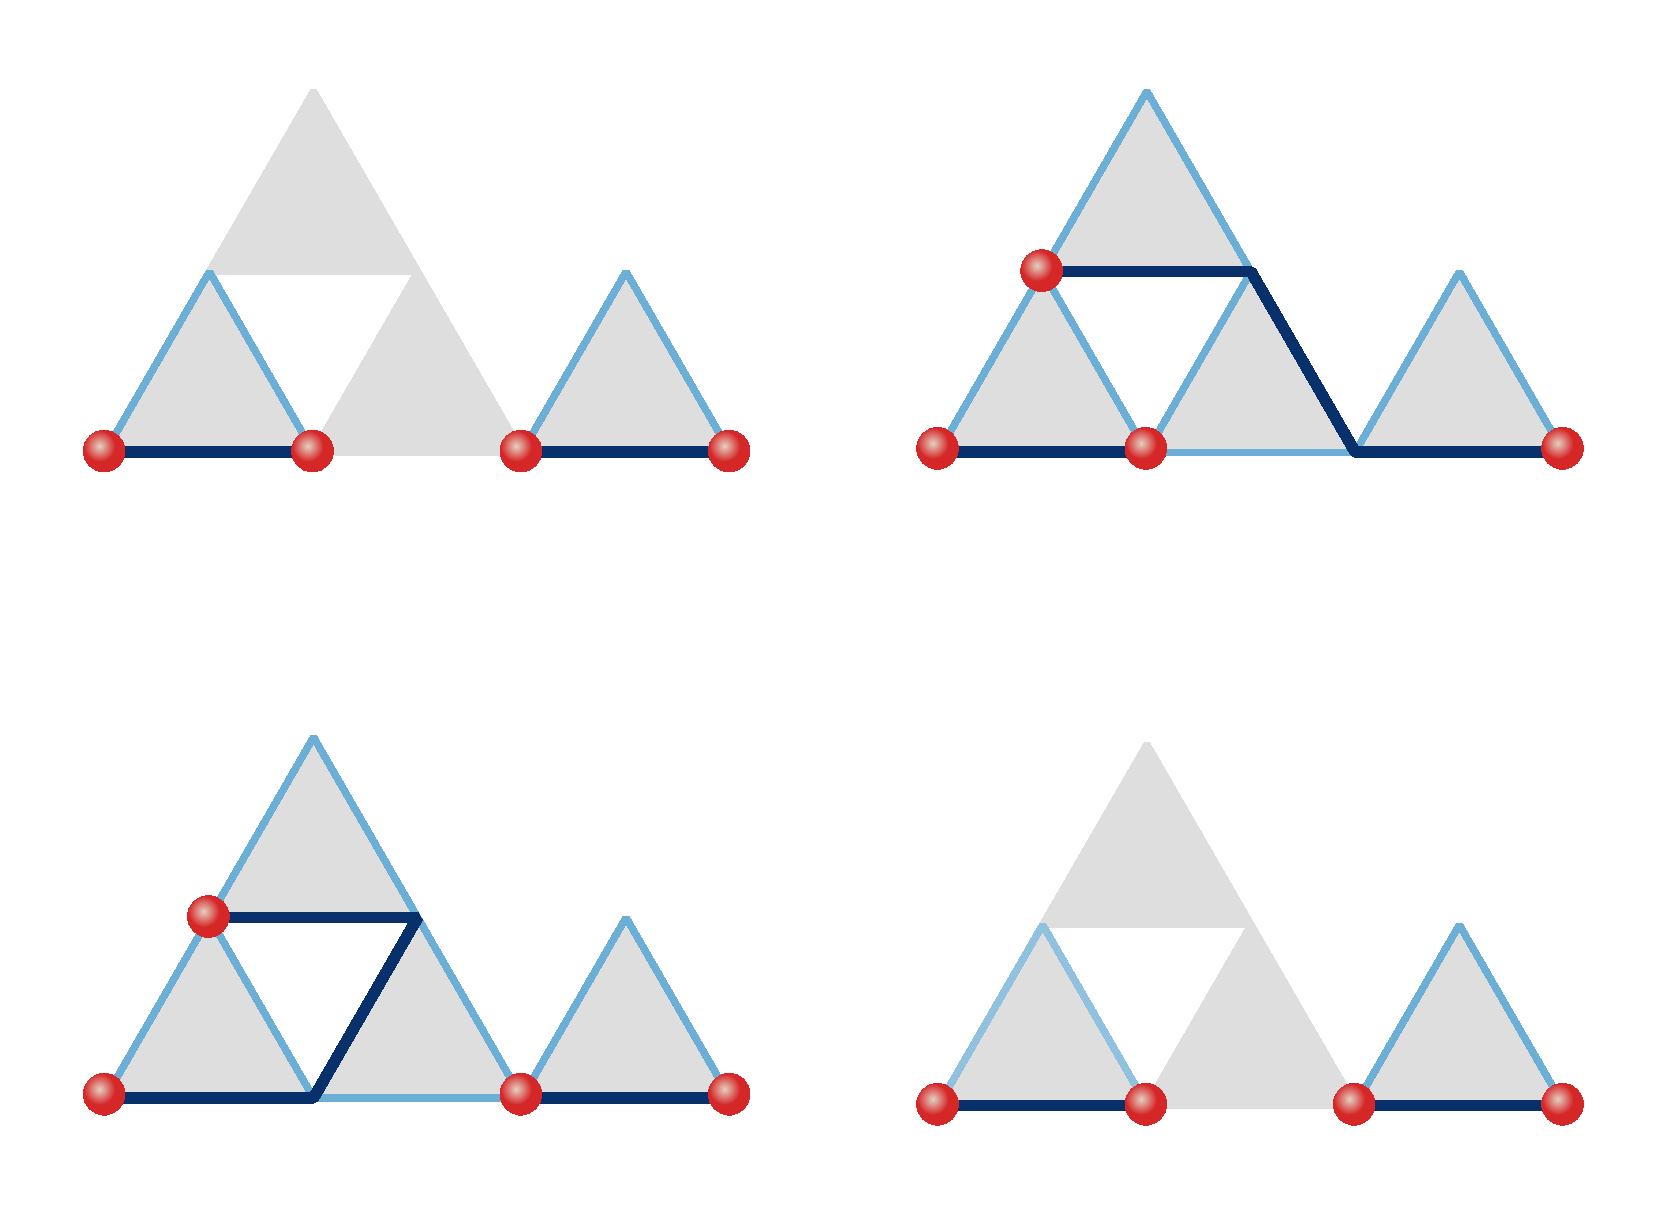
\includegraphics[width=0.90\textwidth]{./figures/4-mf-swap-2-3.pdf}};

    \node[inner sep=0pt] (a) at (-8,5.50) {(a)};
    \node[inner sep=0pt] (b) at (0.2,5.50) {(b)};
    \node[inner sep=0pt] (c) at (-8,-.50) {(c)};
    \node[inner sep=0pt] (d) at (0.2,-.50) {(d)};

    \node[inner sep=0pt] (gamma1) at (-6.6,0.95) {$\gamma_1$};
    \node[inner sep=0pt] (gamma2) at (-4.6,0.95) {$\gamma_2$};
    \node[inner sep=0pt] (gamma3) at (-2.8,0.95) {$\gamma_3$};
    \node[inner sep=0pt] (gamma4) at (-0.9,0.95) {$\gamma_4$};

    \node[inner sep=0pt] (gamma1) at (0.90,0.95) {$\gamma_1$};
    \node[inner sep=0pt] (gamma2) at (2.80,0.95) {$\gamma_2$};
    \node[inner sep=0pt] (gamma3) at (1.4,3.50) {$\gamma_3$};
    \node[inner sep=0pt] (gamma4) at (6.50,0.95) {$\gamma_4$};

    \node[inner sep=0pt] (gamma1) at (-6.6,-4.80) {$\gamma_1$};
    \node[inner sep=0pt] (gamma3) at (-6.0,-2.30) {$\gamma_3$};
    \node[inner sep=0pt] (gamma2) at (-2.8,-4.80) {$\gamma_2$};
    \node[inner sep=0pt] (gamma4) at (-0.9,-4.80) {$\gamma_4$};

    \node[inner sep=0pt] (gamma1) at (0.90,-4.80) {$\gamma_1$};
    \node[inner sep=0pt] (gamma3) at (2.80,-4.80) {$\gamma_3$};
    \node[inner sep=0pt] (gamma2) at (4.60,-4.80) {$\gamma_2$};
    \node[inner sep=0pt] (gamma4) at (6.60,-4.80) {$\gamma_4$};

  \end{tikzpicture}
  \caption{Representative steps for braiding four MZM in four triangles sharing corners. (a) Initialization of four MZM $\gamma_1, \gamma_2, \gamma_3, \gamma_4$. All three edges of the bottom-middle and the top triangles are in the trivial phase by e.g. controlling the chemical potential. The bottom-left and bottom-right triangles have $\varphi = 0$ so that their bottom edges are nontrivial. (b) Moving $\gamma_3$ by ``switching on" the middle triangle by changing the chemical potential under a fixed vector potential at $\varphi=\frac{\pi}{6}$, and then turning on the top triangle with similar means except $\varphi = 0$. (c) Transporting $\gamma_2$ to the right triangle through rotating the vector potential in the middle triangle counterclockwise by $\pi/6$. (d) Moving $\gamma_3$ to the left triangle by ``switching off" the top triangle followed by the middle triangle.}
  \label{fig:4MZMbraiding}
\end{figure}

For possible physical realizations of our triangles, immediate choices are quantum dots forming a Kitaev triangle \cite{dvirRealizationMinimalKitaev2023}, planar Josephson junctions or cuts on quantum anomalous Hall insulator/superconductor heterostructures \cite{xieCreatingLocalizedMajorana2021} that form a hollow triangle, and triangular atomic chains assembled by an STM tip \cite{schneiderPrecursorsMajoranaModes2022} on a close-packed surface. The quantum-dot platform may be advantageous in the convenience of implementing parity readout by turning the third vertex temporarily into a normal quantum dot \cite{mishmashDephasingLeakageDynamics2020,parity_QD_readout_2020, fengProbingRobustMajorana2022}. Looking into the future, it is more intriguing to utilize the spontaneously formed triangular islands in epitaxial growth \cite{pietzschSpinResolvedElectronicStructure2006} with the center region removed either physically by lithography/ablation, or electrically by gating. To create a staggered vector potential or supercurrent profile for the Kitaev triangle, one can use a uniform magnetic field, corresponding to a constant vector potential gradient, plus a uniform supercurrent that controls the position of the zero. It is also possible to use two parallel superconducting wires with counter-propagating supercurrents proximate to the triangle.

A tentative design for braiding more than two MZM, illustrated in Fig.~\ref{fig:4MZMbraiding}, consists of four triangles sharing corners with their neighbors. The critical step of transporting $\gamma_2$ to the left vertex of the rightmost triangle, corresponding to Figs.~\ref{fig:4MZMbraiding} (b,c), can be achieved by rotating the vector potential of the bottom-middle triangle counterclockwisely from $\varphi = \frac{\pi}{6}$ to $\frac{\pi}{3}$, which swaps the topological phases of the two side edges as shown in Fig.~\ref{fig: rotation}. In \cite{supp} we show this operation does not involve gap closing at least for certain parameter regions. Our work provides a versatile platform for manipulating MZM based on currently available candidate MZM systems and for potentially demonstrating the non-Abelian nature of MZM in near-term devices.


\chapter{Floquet Landau Levels}

\section{Introduction}

For more than twenty years, Majorana zero modes (MZM) in condensed matter systems have been highly sought after due to their potential for serving as building blocks of topological quantum computation, thanks to their inherent robustness against decoherence and non-Abelian exchange statistics \cite{ivanovNonAbelianStatisticsHalfQuantum2001, kitaevFaulttolerantQuantumComputation2003, nayakNonAbelianAnyonsTopological2008, aliceaNonAbelianStatisticsTopological2011, aasenMilestonesMajoranaBasedQuantum2016}. MZM were originally proposed to be found in half-quantum vortices of two-dimensional (2D) topological \textit{p}-wave superconductors and at the ends of 1D spinless \textit{p}-wave superconductors \cite{readPairedStatesFermions2000, kitaevUnpairedMajoranaFermions2001}. Whether a pristine \textit{p}-wave superconductor \cite{brisonPWaveSuperconductivityDVector2021} has been found is still under debate. However, innovative heterostructures proximate to ordinary $s$-wave superconductors have been proposed to behave as effective topological superconductors in both 1D and 2D. These include, for example, semiconductor nanowires subject to magnetic fields \cite{mourikSignaturesMajoranaFermions2012, rokhinsonFractionalJosephsonEffect2012, dengAnomalousZeroBiasConductance2012}, ferromagnetic atomic spin chains \cite{choyMajoranaFermionsEmerging2011, brauneckerInterplayClassicalMagnetic2013, klinovajaTopologicalSuperconductivityMajorana2013,nadj-pergeProposalRealizingMajorana2013,nadj-pergeObservationMajoranaFermions2014,schneiderPrecursorsMajoranaModes2022}, 3D topological insulators \cite{fuSuperconductingProximityEffect2008, hosurMajoranaModesEnds2011, potterEngineeringMathitipSuperconductor2011, veldhorstMagnetotransportInducedSuperconductivity2013}, quantum anomalous Hall insulators \cite{chenQuasionedimensionalQuantumAnomalous2018, zengQuantumAnomalousHall2018, xieCreatingLocalizedMajorana2021}, quasi-2D spin-orbit-coupled superconductors with a perpendicular Zeeman field \cite{oregHelicalLiquidsMajorana2010, sauGenericNewPlatform2010, lutchynSearchMajoranaFermions2011, potterTopologicalSuperconductivityMajorana2012, liTwodimensionalChiralTopological2016, leiUltrathinFilmsSuperconducting2018}, and planar Josephson junctions \cite{black-schafferMajoranaFermionsSpinorbitcoupled2011, pientkaSignaturesTopologicalPhase2013, hellTwoDimensionalPlatformNetworks2017, fornieriEvidenceTopologicalSuperconductivity2019, renTopologicalSuperconductivityPhasecontrolled2019, scharfTuningTopologicalSuperconductivity2019, zhouPhaseControlMajorana2020}, etc. It has been a challenging task to decisively confirm the existence of MZM in the various experimental systems due to other competing mechanisms that can potentially result in similar features as MZM do in different probes \cite{xuExperimentalDetectionMajorana2015, albrechtExponentialProtectionZero2016, sunMajoranaZeroMode2016, wangEvidenceMajoranaBound2018, jackObservationMajoranaZero2019, fornieriEvidenceTopologicalSuperconductivity2019, renTopologicalSuperconductivityPhasecontrolled2019, mannaSignaturePairMajorana2020}. Other proposals for constructing Kitaev chains through a bottom-up approach, based on, e.g. magnetic tunnel junctions proximate to spin-orbit-coupled superconductors \cite{fatinWirelessMajoranaBound2016}, and quantum dots coupled through superconducting links \cite{sauRealizingRobustPractical2012,leijnseParityQubitsPoor2012,dvirRealizationMinimalKitaev2023} are therefore promising. In particular, the recent experiment \cite{dvirRealizationMinimalKitaev2023} of a designer minimal Kitaev chain based on two quantum dots coupled through tunable crossed Andreev reflections (CAR) offers a compelling route towards MZM platforms based on exactly solvable building blocks.

In parallel with the above efforts of realizing MZM in different materials systems, scalable architectures for quantum logic circuits based on MZM have also been intensely studied over the past decades. A major proposal among these studies is to build networks of T-junctions, which are minimal units for swapping a pair of MZM hosted at different ends of a junction, that allow braiding-based TQC \cite{aasenMilestonesMajoranaBasedQuantum2016}. Alternatively, networks based on coupled wires forming the so-called tetrons and hexons, aiming at measurement-based logic gate operations  \cite{karzigScalableDesignsQuasiparticlepoisoningprotected2017}, have also been extensively investigated. To counter the technical challenges of engineering networks with physical wires or atomic chains, various ideas based on effective Kitaev chains, such as quasi-1D systems in thin films \cite{potterMultichannelGeneralizationKitaev2010}, cross Josephson junctions \cite{zhouPhaseControlMajorana2020}, scissor cuts on a quantum anomalous Hall insulator \cite{xieCreatingLocalizedMajorana2021}, and rings of magnetic atoms \cite{liManipulatingMajoranaZero2016}, etc. have been proposed. However, due to the same difficulty of obtaining or identifying genuine MZM in quasi-1D systems mentioned above, it remains unclear how practical these strategies are in the near future.

In this Letter, we propose an alternative structural unit for manipulating MZM, triangular superconducting islands, motivated by the above challenges associated with wire geometries and by the fact that triangular islands routinely appear spontaneously in epitaxial growth \cite{pietzschSpinResolvedElectronicStructure2006} on close-packed atomic surfaces. We first show that a minimal ``Kitaev triangle'' consisting of three sites hosts MZM at different pairs of vertices controlled by Peierls phases on the three edges [Fig.~\ref{fig:triangles} (a)], which can be readily realized using quantum dots. To generalize the minimal model to triangular structures involving more degrees of freedom, we study the topological phase transitions of quasi-1D ribbons driven by Peierls phases, which can be created by magnetic fields or supercurrents \cite{romitoManipulatingMajoranaFermions2012, takasanSupercurrentinducedTopologicalPhase2022}, and use the resulting phase diagram as a guide to construct finite-size triangles with a hollow interior that host MZM  [Fig.~\ref{fig:triangles} (b)]. In the end we discuss possible experimental systems that can realize our proposals and scaled-up networks of triangles for implementing braiding operations of MZM.



\section{Floquet LLs in 2DEG}
We consider the case of Schr\"{o}dinger electrons under the application of two linearly polarized laser lights. The unperturbed Hamiltonian for 2DEG is%
\begin{equation}\label{eq:H2DEG}
H=\frac{\pi_{x}^{2}}{2m^{\ast}}+\frac{\pi_{y}^{2}}{2m^{\ast}},
\end{equation}
where $m^{\ast}$ is the effective mass of electron. By changing the Hamiltonian into a time-dependent form by applying two linearly polarized lights
such that $\bm{\pi}\rightarrow \vec{p}-q\vec{A}(t)$. \ Therefore, Eq.~\eqref{eq:H2DEG} is written as%
\begin{equation}\label{eq:H2time}
H(t)=\frac{1}{2m^{\ast}}[p_{x}-qA_{x}(t)]^{2}+\frac{1}{2m^{\ast}}[p_{y} -qA_{y}(t)]^{2},
\end{equation}
where the electric field components for two spatially inhomogeneous linearly polarized laser lights are
\begin{align} \label{eq:E2field}
  \vec{E}_{1} &= E\sin{(Kx)} \cos{(\omega t)}\hat{x}, \nonumber \\
  \vec{E}_{2} &= -E\sin{(Kx)} \sin{(\omega t)}\hat{y}.
\end{align}%
The field given in Eq.~\eqref{eq:E2field} lead to the following vector potential $\vec{A}(t)$
\begin{equation}\label{eq:Avec2deg}
  \vec{A}(t)= -\dfrac{E}{\omega} \sin{(Kx)} \left\langle \sin (\omega t), \cos{(\omega t)},0 \right\rangle.
\end{equation}%
Substituting into the Schrodinger Hamiltonian we arrive at

\begin{align}\label{eq:Htime2deg}
  \ham(t) = \dfrac{1}{2m} [ &p_x^2 + p_y^2 + V^2 \sin^2{(Kx)} + V^2 \sin{(\omega t)} (p_x \sin(Kx) + \sin(Kx) p_x) + 2Vp_y \sin(Kx) \cos(\omega t) ]
\end{align}
where $V=qE/\omega$.
Because of the time-translation symmetry through $A(t+T) = A(t)$ with $T = 2\pi/\omega$, one can apply the Floquet theory \cite{AEE, MBL, supp} and obtain an effective Hamiltonian from Eq.~\eqref{eq:Htime2deg}. After performing the Fourier transform of the time-periodicity, first order expansion in $\hbar \omega$ terms and in the long wavelength limit leads to the final effective Hamiltonian as

\begin{align}\label{eq:Heff2deg}
  \ham_{\rm eff} &= \dfrac{1}{2m} \left[ p_x^2 + p_y^2 + V^2K^2x^2 + \dfrac{\hbar V^2}{4m\omega} (K^2 - 2K^4x^2) - \dfrac{2V^2K^2}{m\omega} p_y x \right] \nonumber \\
  \ham &= \dfrac{1}{2m} \left[ p_x^2 + p_y^2 - \dfrac{2V^2K^2}{m\omega} p_y x + \left(1-\dfrac{\hbar K^2}{2m\omega}\right)V^2K^2x^2 + \dfrac{\hbar V^2 K^2}{4m\omega} \right]
\end{align}
Notice here we have quantum harmonic oscillator (QHO) in x-axis and also coupling between $p_y$ and $x$.
The coupling can allow for flux pumping.
While we may have Landau levels, from the QHO, it still needs to be shown if our system has topological edge states.

\subsection{2DEG Numerical Approach}

We now consider a 2D square lattice tight-binding model.
The incident laser light doesn't allow for translation symmetry along the x-axisin which we will only consider a finite radius along the x-axis and treat the y-axis as infinite.
Our unit cell will still only contain one atom per cell, this will not be the case for Dirac.
Lattice vectors are described as follows $\vec{a}_1 = a\hat{x}$, and $\vec{a}_2 = a \hat{y}$.
We will use a Peierls phase to introduce the vector potential field to the tight-binding Hamiltonian.
In general, the Hamiltonian has the following form:
\begin{equation}
  \ham(t) = -\sum_{jl} h_{j,j+1}(t) \cc_{j,l} c_{j+1,l} + h_{l,l+1} \cc_{j,l} c_{j,l+1} + h.c.
\end{equation}
where $h$, hopping amplitude, takes the following phase contributions

\begin{align}
  h_{j,j+1}(t) &= \exp \left[ i \dfrac{qE}{\hbar \omega}(x_{j+1}-x_j) \sin(K\bar{x}_{j,j+1}) \sin{\omega t} \right] \nonumber \\
  h_{j,j+1}(t) &= \exp \left[ i Z_1 \sin{\omega t} \right] \\
  h_{j+1,j}(t) &= \exp \left[ -i Z_1 \sin{\omega t} \right] \\
h_{l,l+1}(t) &= \exp \left[ i \dfrac{qE}{\hbar \omega} (y_{l+1}-y_l) \sin(Kx_j) \cos\omega t \right] \nonumber \\
  h_{l,l+1}(t) &= \exp \left[ i Z_2 \cos\omega t \right] \\
  h_{l+1,l}(t) &= \exp \left[ -i Z_2 \cos\omega t \right]
\end{align}
where $Z = qEa/\hbar \omega$, $Z_1 = Z\sin(K\bar{x}_{j,j+1})$, $Z_2 = Z\sin(Kx_j)$, and $\bar{x}_{j,j+1} = (x_{j+1}+x_j)/2$.
One can fourier transform along the y-axis to momentum space to simplify the system to

\begin{align}
  \ham(t) &= -\sum  h e^{iZ_1\sin{\omega t}} \cc_{jk} c_{j+1,k} + h e^{ i Z_2 \cos(\omega t) - ika} \cc_{jk} c_{jk} + h.c. \nonumber \\
  &= -\sum_{jk} h_{j,j+1}(t) \cc_{jk} c_{j+1,k} + h_{jk}(t) \cc_{jk} c_{jk} + h.c.
\end{align}

We next impose Floquet theory and take fourier time-domain transforms of the Hamiltonian.
Both of the terms take the following form

\begin{align}
  h_{j,j+1,n} &= \dfrac{1}{T} \int_0^T h_{j,j+1}(t) e^{-in\omega t} dt \nonumber \\
  &= \dfrac{h}{T} \int_0^T e^{iZ_1 \sin{\omega t} -in\omega t} dt \nonumber \\
  &= \dfrac{h}{2\pi} \int_0^{2\pi} e^{iZ_1 \sin\tau - in\tau} d\tau \nonumber \\
  &= h J_n(Z_1) \\
  h_{j+1,j,n} &= h (-1)^n J_n(Z_1)
\end{align}

\begin{align}
  h_{jk,n} &= \dfrac{1}{T} \int_0^T h_{jk}(t) e^{-in\omega t} dt \nonumber \\
  &= \dfrac{h}{T} e^{-ika} \int_0^T e^{- iZ_2 \cos{(\omega t)} - in\omega t} dt \nonumber \\
  &= \dfrac{h}{2\pi} e^{-ika} \int_0^{2\pi} e^{-i Z_2\cos\tau - in\tau} d\tau \nonumber \\
  &= \dfrac{h}{2\pi} e^{-in\pi/2-ika} \int_0^{2\pi} e^{-iZ_2 \cos\tau - in\tau + in\pi/2} d\tau \nonumber \\
  &= he^{- in\pi/2 -ika} J_{n}(Z_2) \\
  h_{jk,n}^* &= he^{+ in\pi/2 +ika} J_{n}(Z_2)
\end{align}
The Hamiltonian after fourier transform is

\begin{equation}
  H_n = -h \sum_{jk} J_n(Z_1) \left(\cc_{jk} c_{j+1,k} + (-1)^n \cc_{j+1,k} c_{jk}\right) + 2\cos\left(ka+\tfrac{n\pi}{2}\right) J_n(Z_2) \cc_{jk} c_{jk}
\end{equation}

We now build the quasienergy matrix $\bar{Q}$ that has matrix elements

\begin{equation}
  \bar{Q}_{m,m+n} = H_n - m\hbar\omega \delta_{n0}
\end{equation}
The quasienergy matrix by definition is infinite in Floquet theory and thus not possible to solve at least numerically.
However, since we are interested in the behavior at zeroth mode and depending on the stregnth of laser light energy, $\hbar\omega$, we choose a cutoff mode $|m|\leq m_c$, where $m_c$ is a positive integer such that higher modes do not contribute to the zeroth modes behavior.
Notice we have two cutoffs, one for x-axis radius and for light modes.
This translates to a matrix with dimensions ${(N_r N_m)}^2$, $N_r = (2*r_c+1)$, and $N_m=(2*m_c+1)$.


\section{Floquet Landau level-like bands in Dirac systems}
In this section we demonstrate a Dirac system in the presence of a standing, non-uniform, circularly polarized light becomes an effective Dirac Hamiltonian with a magnetic field that is composed of the electric field component of light.
Dirac electrons can be represented with a generic model 2D Hamiltonian honeycomb monolayer in the presence of a gauge potential as

\begin{figure}
  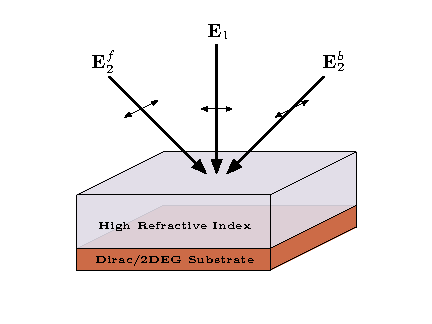
\includegraphics[width=0.5\textwidth]{./figures/fll-setup.pdf}
  \caption{Schematic of two oblique (forward and backward) and one normally incident light on graphene or a 2DEG substrate with high refractive index material on top. Oblique lasers have polarization in $y$-axis and travel in $xz$-plane and normally incident laser has polarization in the $x$-axis and travel in $yz$-plane. With beam width large enough to cover the device fully.}
  \label{fig:fll-setup}
\end{figure}

\begin{equation}\label{eq:HDirac}
  \ham(t) = v_{F} \bm{\sigma} \cdot \left(\vec{p} + e\vec{A}(t)\right),
\end{equation}
where $\vec{A}$ is the gauge potential, $\vec{p}$ is the momentum operator, $v_F$ is the Fermi velocity of Dirac fermions, $e$ is electron charge, and $\vec{\sigma}$ the Pauli matrices vector in 2D.
The light is made of three linearly polarized lasers, as shown in Fig. \ref{fig:fll-setup}.
Where the first is normally incident in the $z$-axis with polarization in the $x$-axis.
The second and third are of oblique incidence in the $xz$-plane, to acquire non-uniformity in the $x$-axis, with polarization in the $y$-axis, and mirrored about the $yz$-plane.
This is to introduce $x$-dependence with the $p_y$ term of the Dirac Hamiltonian.
The relevant electric field components at the Dirac system interface are

\begin{align} \label{eq:EDfield}
\vec{E}_{1} &= E\cos \omega t\ \hat{x}, \nonumber \\
\vec{E}_{2} &= \vec{E}_2^f + \vec{E}_2^b = E\sin(Kx)\sin 2\omega t\ \hat{y},
\end{align}
%Where $\omega$ is angular frequency of light with time $t$ and $K=2\pi /d$ with $d$ being the spatial period of the electric field with amplitude $E$.
Where $\omega$ is angular frequency of the laser with time $t$ and $K = \omega \sin{(\theta_i)} / v_p$, with $\theta_i$ as incident angle of the oblique lasers and $v_p$ is phase velocity of the lasers.
%Notice, the second electric field has twice frequency of the first, this is a requirement to make the Dirac Hamiltonian into a Landau level-like Hamiltonian, the derivation in REFERENCE APPENDIX can inform the reader of this choice.
Notice, the second electric field has twice frequency of the first, this allows for the second gauge potentials $\sigma_y$ to have non-zero commutation with the first gauge potentials $\sigma_x$, and due to the high-frequency expansion used later, allows for the second gauge potential to return to a $\sigma_y$, as seen in \ref{fll-dirac-derivation}.
This form of the electric field relates to the following gauge potential, via $\vec{E} = -\partial_t \vec{A}$ as

\begin{equation}\label{eq:ADirac}
  \vec{A}(t)= \dfrac{E}{\omega} \left\langle -\sin \omega t, \tfrac{1}{2}\sin(Kx) \cos 2\omega t \right\rangle,
\end{equation}%
Substituting Eq.~\eqref{eq:ADirac} into Eq.~\eqref{eq:HDirac}, we arrive at%

\begin{equation}\label{eq:HDtime}
  \ham(t)= v_{F}\bm{\sigma}\cdot\vec{p} - \sigma _{x} \dfrac{v_F eE}{\omega} \sin {\omega t} - \sigma _{y} \dfrac{v_F eE}{2\omega}\sin{(Kx)} \cos2\omega t.
\end{equation}%
Due to the laser's time-translation symmetry through $A(t+T)=A(t)$ with $T=2\pi /\omega $, one can apply the Floquet theory \cite{AEE, MBL, supp} and obtain an effective Hamiltonian from Eq.~\eqref{eq:HDtime}.
This introduces the quasienergy matrix $Q_{m,m+n} = H_n + m\hbar\omega\delta_{n0}$ after performing the Fourier time-transform of the Hamiltonian, given as

\begin{equation} \label{eq:fourier-time-transform}
  H_n = \dfrac{1}{T} \int_{0}^{T} \ham(t) e^{-in\omega t} dt,
\end{equation}
then we are left with modes $m=0,\pm1,\pm2$.
To use the high-frequency approximation we require $\hbar\omega \gg H_{\pm1,\pm2}$, the off-diagonal terms.
After applying the high-frequency approximation to first and second order expansion in $\hbar\omega$, it leads to the zeroth-mode effective Hamiltonian in Eq.~\eqref{eq:HDtime} as

\begin{equation} \label{eq:HDeff}
  H_{\text{eff}}= v_{F}\bm{\sigma}\cdot\vec{p}-\sigma_y\frac{v_F^3 e^2 E^2 p_y}{\hbar^{2}\omega^{4}}
  +\sigma_y\frac{v_F^3 e^3 E^{3}\sin{(Kx)}}{4\hbar^{2}\omega^{5}}
  -\sigma_x\frac{v_F^3 e^2 E^2 \left\{p_x, \sin^2{(Kx)} \right\} }{8\hbar^{2}\omega^{4}}.
\end{equation}
The derivation can be found in the Appendix \ref{fll-dirac-derivation}.
This effective Hamiltonian can be simplified in the long wavelength limit, $Kx \ll 1$ to

\begin{align} \label{eq:HeffDirac}
  %\ham_{\text{eff}} &= v_F \sigma_x p_x + v_F \sigma_y \left[ \left( 1- \dfrac{v_F^2e^2E^2}{\hbar^2\omega^4} \right) p_y + \dfrac{K v_F^2 e^3 E^3}{4 \hbar^2 \omega^5} x \right] \nonumber \\
  \ham_{\text{eff}}^D &= v_{F}\sigma_{x}p_{x}+v_F\sigma_{y} \left( C p_{y} + eB^Dx \right),
\end{align}%
where $C = 1-\left(\tfrac{v_{F}eE}{\hbar\omega^2}\right)^2$ and $B^D=\frac{Kv_F^2 e^2E^3}{4\hbar^{2}\omega^{5}}$.
%In accordance with Eqs.~\eqref{eq:HDeff} and ~\eqref{eq:HeffDirac}, there is least anisotropy in the Dirac spectrum in addition to zero gap.
Diagonalizing the Hamiltonian in Eq.~\eqref{eq:HeffDirac}, we obtained the eigenvalues for Dirac system as%

\begin{equation} \label{eq:DiracEner}
  \epsilon_{n}^D = \pm v_F^2 \sqrt{\dfrac{nK e^3 E^3}{2 \hbar \omega^5}}
\end{equation}
which is similar to graphene LLs spectrum in the limit of equal velocities.
The effective magnetic field in the Dirac Hamiltonian achieves a highly degenerate energy spectrum similar to LLs.
Unlike conventional LLs, the electron motion is not a cyclotron orbit but a potentially more complicated orbit, due to CPL inducing a Coulumb force in the material's 2D plane.
In Eq. ~\eqref{eq:HDeff}, the first order term in $\hbar \omega$ leads to gap at the Dirac point in normally incident, circularly polarized light experiments \cite{YHW, JWM} and is zero here due to the non-uniformity nature of oblique incident lasers.

There are several ways to enhance the effective magnetic field and directly LL-like energies for a Dirac system.
Electric field strength can be increased within reason as we are limited by the photon energy to ensure the high-frequency expansion holds, $E \ll 2\hbar\omega^2/e v_F$.
One can reasonably use electric field strengths up to 20\% of the limit due to photon energy.
The laser wavenumber $K= \omega \sin{(\theta_i)} / v_p$ has a linear relationship to photon energy, too.
Overall, considering the high-frequency limit on the electric field, the effective field $B^D \propto \omega^2 \sin{(\theta_i)} / (v_F v_p)$.
Without too much consequence the incident angle can be increased up to $\pi/2$ and decreasing the phase velocity of light would enhance the effective magnetic field.
Increasing photon energy is one way to enhance the effective magnetic field.
As considered in previous literature, when photon energy and electric field are increased more energy is pumped into the system, shorter pulses are required to prevent damaging the system \cite{YHW, JWM}.

%\Blue{This next paragraph should be in the discussion since it uses similar language and results as 2DEG?}
%It is important to note, that this system experiences QHE for values of $C\neq0$ and can flip chirality when $C$ changes sign, more details in REFERENCE APPENDIX.
%We can have gapped Dirac spectrum and QAHE by using uniform circularly polarized laser light as observed in experiments \cite{YHW, JWM} or by using any substrate like hBN.
%Now, we have shown one can achieve a highly degenerate Landau level-like spectrum and QHE with an effective magnetic field strength which is directly proportional to third order of the electric field and inversely proportional to the product of spatial period and fifth order of the frequency of the polarized light $\propto (E^3/(d\omega^5))$.
%This factor of the laser lights can be tuned and thus effective magnetic field can be enhanced in such nonequilibrium systems.
%In the case of uniform circularly polarized light, one can imagine the Coulomb force makes the charged particles move in a cyclotron orbit.
%In constrast, for non-uniform circularly polarized light, charged particles are not necessarily in cyclotron orbits but in some form of closed orbit preventing the charged particles from moving on average in a given direction, hence we define them as Landau level-lik.

\section{Conclusion}

We now examine the topology of both systems.
Eqs. \eqref{eq:HeffDirac} and \eqref{eq:Heff2deg} are in LL Hamiltonian form, and typically exhibit QHE.
The two systems only have translational symmetry in the $y$-axis, so a Chern number based on periodicity in $k_x$ and $k_y$ is not applicable, though one can relate the center of mass of an electron to the Chern number as shown in Appendix \ref{chern-number}, which is related to the Laughlin pump.
Considering the Laughlin pump argument, both systems have quantized Hall conductivity, since both have the same eigenstates as their respective LL Hamiltonian.
A key difference to note about both systems is the $C$ term in Eq. \eqref{eq:HeffDirac}.
This term will stay positive for the values of $E$ used in the high-frequency limit for the Dirac case.

Using existing experiments \cite{YHW, JWM} we can provide an estimate for the strength of the effective magnetic field to observe LL-like spectrum and QHE.
Analytical structure of Eq.~(\ref{eq:DiracEner}) and Eq.~(\ref{eq:2DEGenergy}) is primarily responsible for the LL-like spectrum in both the Dirac and 2DEG systems, respectively.
Although such results are valid for other 2D materials or Schr\"{o}dinger systems, however, for simplicity, we will consider parameters realized for graphene or topological insulators \cite{YHW, JWM}.
We will consider a similar range of mid-IR photon energies (or $\lambda = [3\mu $m$ , 10\mu $m$]$) as seen in graphene or topological insulators \cite{YHW, JWM} to match with recently proposed high refractive index metamaterial composites \cite{shimFundamentalLimitsRefractive2021}.
In these experiments \cite{YHW, JWM}, the strength of the electric field used is $1 \times 10^7$ V/m to $1 \times 10^8$ V/m, for the parameters used to estimate effective magnetic fields for both systems the largest electric field is around $1.4 \times 10^8$ V/m.
As should be considered, the larger both photon energy and electric field become ultrafast pulses should be used to prevent thermal damage to materials, on the order of $500$ fs.
To note, for the following results we assume a high oblique angle to let $\sin{(\theta_i)} \approx 1$.

To enhance the effective magnetic field, aside from using higher photon energy, reducing the photon phase velocity can see a considerable increase in both systems.
The refractive index materials can be set above graphene, or any Dirac material, such that the laser light can propagate through to reduce its phase velocity.
Germanium refractive index increases monotonically with increasing photon energy, we use a linear interpolation of the refractive index due the small change for the range of photon energies used.
Al-composite metamaterials refractive index is monotonically decreasing with increasing photon energy and we use a linear interpolation here as the data is roughly linear.

\begin{figure}
  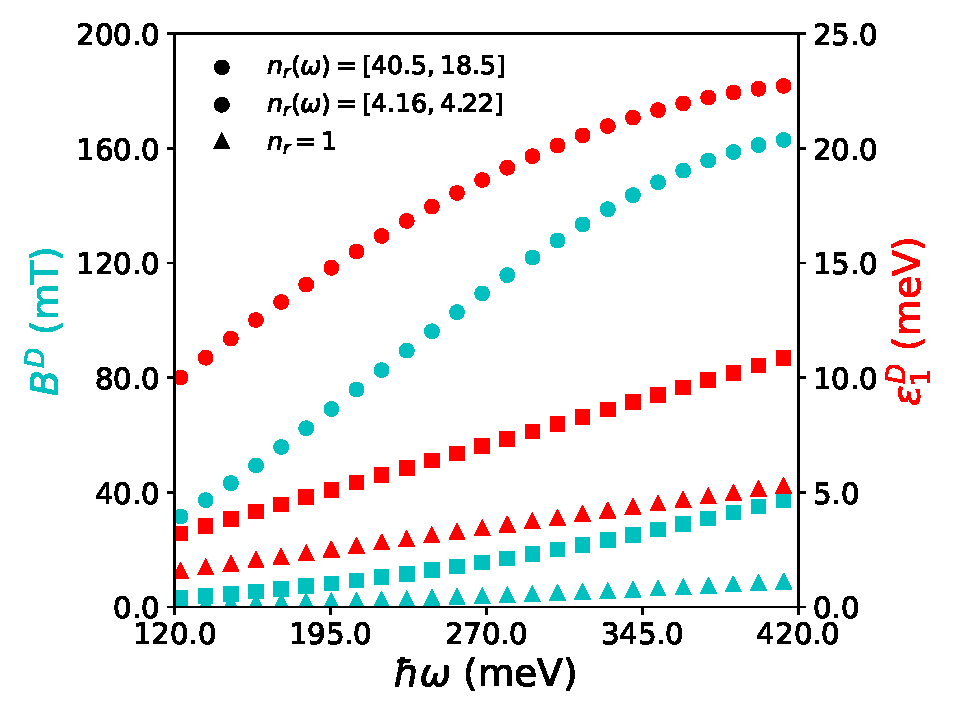
\includegraphics[width=0.45\textwidth]{./figures/dirac-eff-bfield-energy.pdf}
  \caption{Effective magnetic field (cyan) and first quasienergy (red) as a function of photon energy for various refractive materials: vacuum (triangles), germanium (squares), and  Al-composite metamaterial (circles).}
  \label{fig:dirac-bfield-energy}
\end{figure}

In case of a Dirac system Fig. \ref{fig:dirac-bfield-energy} shows graphene with various refractive index materials to enhance the effective magnetic field and first order quasienergy of the LL-like spectrum.
For mid-IR ranges of laser light, the effective magnetic field (cyan) can get up to $8.8$ mT for vacuum, $37.2$ mT for germanium, and $163$ mT for Al-composite metamaterial for $\hbar\omega=413$ meV and results in first order quasienergies (red) of $5.3$ meV, $11$ meV, and $23$ meV, respectively.
As can be seen in \ref{fig:dirac-bfield-energy} as photon energy increases the Al-composite refractive index decreases quite a bit and if we used higher energy we would see the effective magnetic field and quasienergies start to decrease, as will be seen with 2DEG.
While the material has higher index of refraction overall, it would be better to find a material that increases refractive index with photon energy, like germanium can, for it can drastically increase for slightly higher photon energies before effective magnetic field dips \cite{amotchkinaCharacterizationEbeamEvaporated2020}.

\begin{figure}
  \subfloat[]{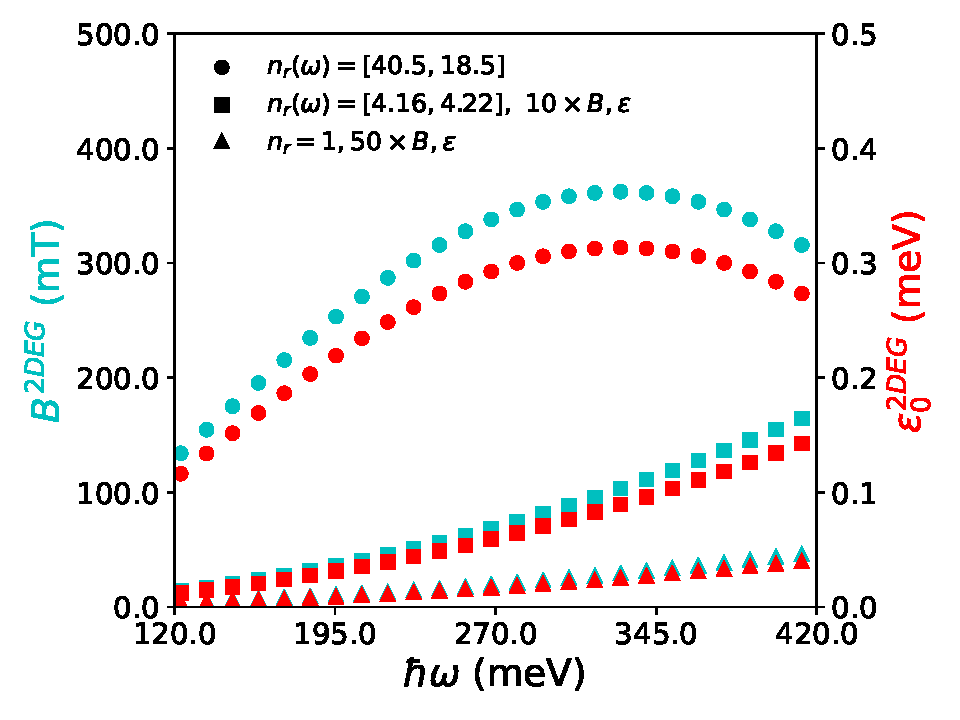
\includegraphics[width=0.45\textwidth]{./figures/2deg-eff-bfield-energy-GaAs.pdf}}
  \subfloat[]{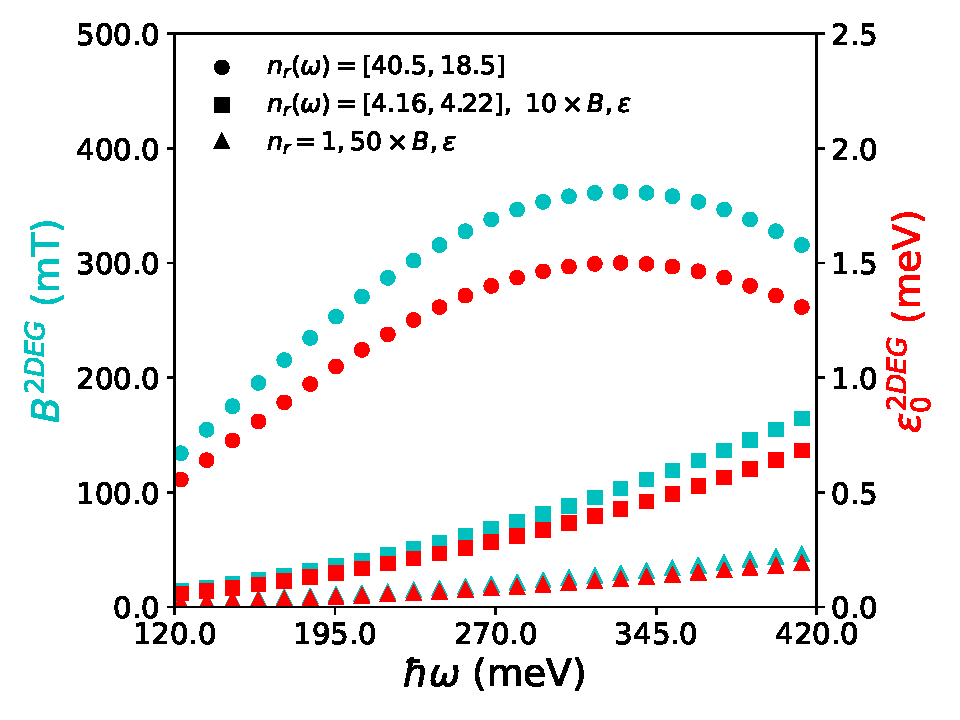
\includegraphics[width=0.45\textwidth]{./figures/2deg-eff-bfield-energy-InSb.pdf}}
  \caption{Effective magnetic field (cyan) and first quasienergy (red) as a function of photon energy for 2DEGs for various refractive materials: vacuum (triangles) scaled by a factor of 50, germanium (squares) scaled by a factor of 10, and Al-composite metamaterials. The 2DEG materials used are (a) GaAs and (b) InSb.}
  \label{fig:2deg-bfield-energy}
\end{figure}

For 2DEG systems Fig. \ref{fig:2deg-bfield-energy} shows GaAs and InSb materials with the same refractive materials used for graphene to enhance effective magnetic field and zeroth order quasienergy of the LL-like spectrum.
The vacuum and germanium interfaces are scaled up by a factor of $10$ and $50$, respectively, to visually enhance and compare it to the Al-composite interface.
GaAs is used as it is one of the most common 2DEG with relatively small effective electron mass, followed by InSb since it has the smallest effective electron mass found in 2DEG materials.
For the GaAs system, effective magnetic field (cyan) can get up to $0.92$ mT for vacuum, $16.5$ mT for germanium, and $362$ mT for Al-composite metamaterial and achieves zeroth order quasienergies (red) of $0.8\ \mu$eV, $14.3\ \mu$eV, and $314\ \mu$eV, respectively.
In the InSb system, effective magnetic field is the same as GaAs, since it has no dependence on effective mass, and achieves zeroth order quasienergies (red) of $3.8\ \mu$eV for vacuum, $68.2\ \mu$eV for germanium, and $1.5$ meV for Al-composite.
As alluded to earlier, due to Al-composites large decrease in refractive index for increasing photon energy, it peaks earlier around $\hbar\omega=328$ mT, for 2DEG.
Overall, we see large changes in 2DEG for both effective magnetic field, due to being proportional to refractive index squared and quasienergies, being inversely proportional to effective electron mass.

There are a few items we did not consider for our calculations.
First, we do not consider any effects due to a refractive index material in contact with a Dirac or 2DEG system.
Secondly, while the high-frequency expansion limits the electric field applied to the materials one could still go beyond the limit of $\hbar \omega \ll H_{pm1}, H_{\pm2}$ to enhance the effective magnetic field by a few orders of magnitude with some error.
For example, if instead we use $\hbar\omega = H_{\pm1}, H_{\pm2}$, this would be multiplying the electric field by a factor of $5$ from our calculations presented, Dirac effective magnetic field would increase by a factor of $125$ while 2DEG effective magnetic field would increase by a factor of $25$.
For Dirac systems with higher electric field strengths, if $C=0$, there would be no QHE as there is no coupling between $x$ and $p_y$, and if $C<0$, the direction of chirality flips.

In conclusion, we have shown Floquet LLs and the QHE using three linearly polarized lights for Dirac and conventional 2DEG systems.
While using these laser lights, we  need at least two polarized lights to be spatially inhomogeneous and mirrored.
We have presented results using frequency space expansion method and degenerate Floquet perturbation theory.
While, a tight-binding model capable of using ``low-frequency'' with a Peierls substitution can be found in appendix \ref{app:tbm-dirac} and \ref{app:tbm-2deg}, the results are difficult to interpret and currently not informative.
The results agree well to show Floquet LL-like energies in experimentally accessible parameters range.
Also, it is vital to note we are flexible to use different values of the electric field strength, photon energy, or phase velocity to realize QHE and control the strength of the effective magnetic field.
Therefore, we think Floquet LL-like and QHE can be observed in experiments for moderate strength of the spatially inhomogeneous laser lights. Moreover, we expect to open up new avenues for nanoelectronics in nonequilibrium systems.




\chapter{Conclusion and Discussion}

  \Blue{What makes gauge potential unique in creating/tuning/manipulating new topoglical systems}
  \Blue{Applications}


\begin{appendices}

\chapter{Superconducting Triangular Islands}
\section{Kitaev chain}
A pair of Majorana fermions can be defined in terms of spinless operators $a_j, a_j^\dag$, where $j$ labels general quantum numbers, as
\begin{eqnarray}\label{eq:atoc}
	&&c_{2j-1} = a_j+ a_j^\dag\\\nonumber
	&&c_{2j} = -i(a_j - a_j^\dag)
\end{eqnarray}
which are hermitian conjugates of themselves. Conversely,
\begin{eqnarray}\label{eq:ctoa}
	&&a_j =\frac{1}{2} (c_{2j-1} + i c_{2j}),\\\nonumber
	&&a_j^\dag = \frac{1}{2}(c_{2j-1} - i c_{2j})
\end{eqnarray}
For a general mean-field Hamiltonian
\begin{eqnarray}
	H = \sum_{jl} h_{jl} a_j^\dag a_l
\end{eqnarray}
where $h$ is a Hermitian matrix, it can be transformed to the Majorana fermion representation as follows:
\begin{eqnarray}\label{eq:BdGMrep}
	H &=& \frac{1}{4}\sum_{jl} h_{jl} (c_{2j-1} - i c_{2j}) ( c_{2l-1} + i c_{2l})\\\nonumber
	&=& \frac{1}{4}\sum_{jl} (h_{jl} c_{2j-1} c_{2l-1} - i h_{jl} c_{2j} c_{2l-1} + ih_{jl} c_{2j-1} c_{2l} + h_{jl} c_{2j} c_{2l}) \\\nonumber
	&=& \frac{i}{4} \sum_{jl} (c_{2j-1}, c_{2j})\begin{pmatrix}
		-ih_{jl} & h_{jl}\\
		-h_{jl} & -ih_{jl}
	\end{pmatrix}\begin{pmatrix}
	c_{2l-1} \\
	c_{2l}
\end{pmatrix}\\\nonumber
&\equiv&\frac{i}{4}\sum_{mn}A_{mn}c_{m}c_n
\end{eqnarray}
where the matrix $A$ anti-Hermitian since
\begin{eqnarray}
	H^\dag = -\frac{i}{4}\sum_{mn}A_{mn}^* c_n c_m =  H
\end{eqnarray}
which leads to $A_{mn}^* = -A_{nm}$. If the Hamiltonian does not preserve particle number, i.e., it is a BdG Hamiltonian, we have, similarly
\begin{eqnarray}
H = \sum_{jl} \left(h_{jl} a_j^\dag a_l + \Delta_{jl} a_j a_l + \Delta^\dag_{jl}  a_j^\dag a_l^\dag\right)
\end{eqnarray}
supposing we do not double count the terms in the normal part of the Hamiltonian. Then
\begin{eqnarray}
H = \frac{i}{4} \sum_{jl} (c_{2j-1}, c_{2j})\begin{pmatrix}
	-ih -i(\Delta + \Delta^\dag) & h + (\Delta-\Delta^\dag )\\
	-h + (\Delta - \Delta^\dag) & -ih + i(\Delta +\Delta^\dag)
\end{pmatrix}_{jl}\begin{pmatrix}
	c_{2l-1} \\
	c_{2l}
\end{pmatrix}\\\nonumber
\end{eqnarray}
On the other hand, the BdG Hamiltonian can be written as
\begin{eqnarray}\label{eq:HBdG}
	H &=&\frac{1}{2} \sum_{j}h_{jj} + \sum_{jl} \left( \frac{1}{2}h_{jl} a_j^\dag a_l - \frac{1}{2}h_{lj} a_j a_l^\dag + \Delta_{jl} a_j a_l + \Delta^\dag_{jl}  a_j^\dag a_l^\dag \right) \\\nonumber
	&=& \frac{1}{2}{\rm Tr}(h) + \sum_{jl} (a_j^\dag, a_j)\begin{pmatrix}
		\frac{1}{2} h & \Delta^\dag \\
		\Delta & -\frac{1}{2}h^T
	\end{pmatrix}_{jl}\begin{pmatrix}
	a_l \\
	a_l^\dag
\end{pmatrix} \\\nonumber
&\equiv & \frac{1}{2}{\rm Tr}(h) + a^\dag \begin{pmatrix}
	\frac{1}{2} h & \Delta^\dag \\
	\Delta & -\frac{1}{2}h^T
\end{pmatrix} a
\end{eqnarray}
where $a\equiv(a_1, a_2,\dots, a_1^\dag, a_2^\dag,\dots)^T$. Suppose the BdG Hamiltonian can be diagonalized by a Bogoliubov transformation:
\begin{eqnarray}\label{eq:bogoliubov}
	\tilde{a}_j^\dag &=& a_{l}^\dag U_{1,lj} + a_{k} U_{2,kj} \\\nonumber
	\tilde{a}_j &=& a_{l} U^*_{1,lj} + a^\dag_{k} U^*_{2,kj}
\end{eqnarray}
Preserving the anticommutation relation suggests
\begin{eqnarray}
	\delta_{ij} &=& \{\tilde{a}_{i}, \tilde{a}_j^\dag \} = \{a_{l} U^*_{1,li} + a^\dag_{k} U^*_{2,ki},  a_{l'}^\dag U_{1,l'j} + a_{k'} U_{2,k'j}  \} \\\nonumber
	&=&  U^*_{1,li} U_{1,lj} + U^*_{2,ki}U_{2,kj} = (U_1^\dag U_1 + U_2^\dag U_2)_{ij} \\\nonumber
	0 &=& \{\tilde{a}_{i}, \tilde{a}_j \} =\{a_{l} U^*_{1,li} + a^\dag_{k} U^*_{2,ki}, a_{l'} U^*_{1,l'j} + a^\dag_{k'} U^*_{2,k'j}  \} \\\nonumber
	&=& U^*_{1,li}U^*_{2,lj} + U^*_{2,ki}U^*_{1,kj} = (U^\dag_1 U_2^* + U^\dag_2 U_1^*)_{ij}\\\nonumber
	0 &=& \{\tilde{a}_{i}^\dag, \tilde{a}_j^\dag \} =\{a_{l}^\dag U_{1,li} + a_{k} U_{2,ki}, a^\dag_{l'} U_{1,l'j} + a_{k'} U_{2,k'j}  \} \\\nonumber
      &=& U_{1,li}U_{2,lj} + U_{2,ki}U_{1,kj} = (U^\dag_1 U_2^* + U^\dag_2 U_1^*)^*_{ij}
\end{eqnarray}
The above identities simply indicate
\begin{eqnarray}
\mathcal{U} \equiv \begin{pmatrix}
		U_1 & U_2 \\
		U_2^* & U_1^*
	\end{pmatrix}
\end{eqnarray}
is a unitary matrix. Therefore one can diagonalize the BdG Hamiltonian using usual unitary matrices obtained from the eigenvectors of the matrix in the last line of Eq.~\ref{eq:HBdG}:
\begin{eqnarray}\label{eq:HBdGdiag}
	H &=& \frac{1}{2}{\rm Tr}(h) + \tilde{a}^\dag U^\dag \begin{pmatrix}
		\frac{1}{2} h & \Delta^\dag \\
		\Delta & -\frac{1}{2}h^T
	\end{pmatrix} U \tilde{a}\\\nonumber
&\equiv& \frac{1}{2}{\rm Tr}(h) + \frac{1}{2}\tilde{a}^\dag \begin{pmatrix}
	\epsilon & 0 \\
	0 & -\epsilon
\end{pmatrix} \tilde{a}\\\nonumber
&=& \frac{1}{2}\sum_{j}h_{jj} +\frac{1}{2} \sum_{j}(\epsilon_j \tilde{a}_j^\dag \tilde{a}_j - \epsilon_j \tilde{a}_j \tilde{a}_j^\dag) \\\nonumber
&=&  \frac{1}{2}\sum_{j}h_{jj} +\sum_{j}\epsilon_j(\tilde{a}_j^\dag \tilde{a}_j - \frac{1}{2})
\end{eqnarray}
where $\epsilon \equiv {\rm Diag}[\epsilon_1, \epsilon_2,\dots]$. To see why $U$ can transform the BdG Hamiltonian into such a diagonal matrix with opposite eigenvalues at the same positions in the upper-left and lower-right blocks, we check these two terms explicitly
\begin{eqnarray}
	&&\frac{1}{2}(\epsilon_{1} \tilde{a}_j^\dag \tilde{a}_j - \epsilon_{2} \tilde{a}_j \tilde{a}_j^\dag)\\\nonumber
	&=& \frac{\epsilon_1}{2} (a_l^\dag U_{1,lj} + a_k U_{2,kj}) (a_{l'} U^*_{1,{l'}j} + a^\dag_{k'} U^*_{2,k'j}) - \frac{ \epsilon_2 }{2} (a_{l'} U^*_{1,{l'}j} + a^\dag_{k'} U^*_{2,k'j})(a_l^\dag U_{1,lj} + a_k U_{2,kj}) \\\nonumber
	&=& \frac{1}{2}(\epsilon_1 U_{1,lj} U_{1,l'j}^* - \epsilon_2 U^*_{2,lj} U_{2,l'j}) a^\dag_{l} a_{l'} + \frac{1}{2}(\epsilon_1 U_{2,kj} U^*_{2,k'j} -  \epsilon_2 U^*_{1,kj} U_{1, k'j}) a_k a_{k'}^\dag \\\nonumber
	&+& \frac{1}{2} (\epsilon_1 U_{1,lj} U_{2,k'j}^* - \epsilon_2 U_{2,lj}^* U_{1,k'j}) a_{l}^\dag a_{k'}^\dag + \frac{1}{2} (\epsilon_1 U_{2,kj} U^*_{1,l'j} -\epsilon_2 U_{1,kj}^* U_{2,l'j} ) a_{k} a_{l'}
\end{eqnarray}
Comparing them with the original BdG Hamiltonian Eq.~\ref{eq:HBdG}, we can conclude that
\begin{eqnarray}
&&	\epsilon_1 U_{1,lj} U_{1,l'j}^* - \epsilon_2 U^*_{2,lj} U_{2,l'j} = - (\epsilon_1 U_{2,l'j} U^*_{2,lj} -  \epsilon_2 U^*_{1,l'j} U_{1, lj}) \\\nonumber
&& \epsilon_1 U_{1,lj} U_{2,k'j}^* - \epsilon_2 U_{2,lj}^* U_{1,k'j} = (\epsilon_1 U_{2,k'j} U^*_{1,lj} -\epsilon_2 U_{1,k'j}^* U_{2,lj} )^*
\end{eqnarray}
or equivalently
\begin{eqnarray}
	&&(\epsilon_1 - \epsilon_2) (U_{1,lj} U_{1,l'j}^* + U_{2,l'j} U^*_{2,lj} )= 0 \\\nonumber
	&& 0 = 0
\end{eqnarray}
The first equation therefore dictates $\epsilon_1 = \epsilon_2$. However, note that $\epsilon_j$ does not have to be all positive. If the original normal state Hamiltonian can be diagonalized into a form
\begin{eqnarray}
	H = \sum_{j} \tilde{\epsilon}_{j} b^\dag_j b_j
\end{eqnarray}
where $\tilde{\epsilon}_{j}$ can be either positive or negative, the state with the lowest possible energy from the system is
\begin{eqnarray}
	|\Omega \rangle =  \prod_{\tilde{\epsilon}_k < 0} b_k^\dag | 0\rangle
\end{eqnarray}
where $|0\rangle$ is the true vacuum with no particles in any sense. This is the ground state, and its parity is therefore determined by the number of single-particle eigenstates that have negative energies.

From the same perspective, one can define the ground state of the BdG Hamiltonian Eq.~\ref{eq:HBdGdiag} \emph{for a specific set of Fermion operators} $\tilde{a}_j$, as
\begin{eqnarray}
	|\Omega_{\rm BdG}\rangle = \prod_{\epsilon_j < 0} \tilde{a}_j^\dag | 0_{\rm BdG} \rangle
\end{eqnarray}
where $| 0_{\rm BdG} \rangle$ is certain ``vacuum state" for the given set of $\tilde{a}_j$:
\begin{eqnarray}
	\tilde{a}_j | 0_{\rm BdG} \rangle = 0,\, \forall j
\end{eqnarray}
The number of particles in the ground state is therefore determined by the number of negative $\epsilon_j$. However, the sign of $\epsilon_j$ in the present case does not have absolute meaning. For example, supposing $\epsilon_{j_0}<0$, the following Bogoliubov transformation
\begin{eqnarray}\label{eq:Bgtranswitch}
	\tilde{a}'_{j_0} = \tilde{a}_{j_0}^\dag \\\nonumber
	{\tilde{a}}^{\prime \dag}_{j_0} = \tilde{a}_{j_0}
\end{eqnarray}
that only interchanges the creation and annihilation operators for a single $j_0$ and keeps the others unchanged, leads to a different ground state
\begin{eqnarray}
	|\Omega'_{\rm BdG}\rangle = \prod_{\epsilon_j < 0, j\neq j_0} \tilde{a}_j^\dag | 0_{\rm BdG} \rangle
\end{eqnarray}
since the number of negative energy eigenstates decreases by one. The transformation in Eq.~\ref{eq:Bgtranswitch} therefore neither preserves particle number nor particle parity. This can be explicitly checked. The particle number operator in the $\tilde{a}_j$ representation is
\begin{eqnarray}
	N = \sum_{j} \tilde{a}_j^\dag \tilde{a}_j
\end{eqnarray}
Therefore
\begin{eqnarray}
	N' = \sum_{j\neq j_0} \tilde{a}_j^\dag \tilde{a}_j + \tilde{a}_{j_0} \tilde{a}^\dag_{j_0} = N + (1-2 \tilde{a}_{j_0}^\dag \tilde{a}_{j_0})
\end{eqnarray}
The latter equation also means that when the $j_0$ state is occupied in $\Omega_{\rm BdG}$, i.e., $\tilde{a}_{j_0}^\dag \tilde{a}_{j_0} |\Omega_{\rm BdG}\rangle = |\Omega_{\rm BdG}\rangle$, the transformation decreases the total number of particles by 1. Conversely, if it is unoccupied ($\epsilon_{j_0} > 0$), or $\tilde{a}_{j_0}^\dag \tilde{a}_{j_0} |\Omega_{\rm BdG}\rangle = 0$, the transformation increases the particle number by one.

The fermion parity operator can be defined by
\begin{eqnarray}
	P = \prod_j (1-2a_j^\dag a_j)
\end{eqnarray}
so that $P = 1$ if the number of occupied states is even, and $-1$ otherwise. Alternatively, since
\begin{eqnarray}
	a_j^\dag a_j = \frac{1}{4}(c_{2j-1} - ic_{2j})(c_{2j-1} + ic_{2j}) = \frac{1}{2} (1 + ic_{2j-1} c_{2j})
\end{eqnarray}
$P$ can be written in the Majorana representation as
\begin{eqnarray}\label{eq:Pm}
	P = \prod_j (-i c_{2j-1} c_{2j}).
\end{eqnarray}
Eq.~\ref{eq:Bgtranswitch} transforms $P$ by changing
\begin{eqnarray}
	1 - 2\tilde{a}^\dag_{j_0} \tilde{a}_{j_0}\rightarrow 	1 - 2\tilde{a}'_{j_0}\tilde{a}^{\prime\dag}_{j_0} = - (1-\tilde{a}^{\prime\dag}_{j_0}\tilde{a}'_{j_0})
\end{eqnarray}
and hence indeed changes $P$.

We can also understand why the BdG Hamiltonian preserves $P$ but not $N$. Due to the following commutation relations:
\begin{eqnarray}
	&&[a_j^\dag a_{l}, a_j^\dag a_j ] = a_j^\dag a_{l} a_j^\dag a_j - a_j^\dag a_j a_j^\dag a_{l} = - a_j^\dag a_l\\\nonumber
	&&[a_j^\dag a_{l}, a_l^\dag a_l ] = a_j^\dag a_{l} a_l^\dag a_l - a_l^\dag a_l a_j^\dag a_{l} = a_j^\dag a_l\\\nonumber
	&&[a_j^\dag a^\dag_{l}, a_j^\dag a_j ] = a_j^\dag a^\dag_{l} a_j^\dag a_j - a_j^\dag a_j a_j^\dag a^\dag_{l} = - a_j^\dag a_l^\dag\\\nonumber
	&&[a_j^\dag a^\dag_{l}, a_l^\dag a_l ] = a_j^\dag a^\dag_{l} a_l^\dag a_l - a_l^\dag a_l a_j^\dag a^\dag_{l} = - a_j^\dag a_l^\dag\\\nonumber
	&&[a_j a_l, a_j^\dag a_j ] = a_j a_{l} a_j^\dag a_j - a_j^\dag a_j a_j a_{l} =  a_j a_l\\\nonumber
	&&[a_j a_{l}, a_l^\dag a_l ] = a_j a_{l} a_l^\dag a_l - a_l^\dag a_l a_j a_{l} = a_j a_l
\end{eqnarray}
and
\begin{eqnarray}
	[a_j^\dag a_{l}, (1-2a_j^\dag a_j)(1-2a_l^\dag a_l) ] &=& (1-2a_j^\dag a_j)[a_j^\dag a_{l}, (1-2a_l^\dag a_l) ] + 	[a_j^\dag a_{l}, (1-2a_j^\dag a_j)](1-2a_l^\dag a_l) \\\nonumber
	&=& -2(1-2a_j^\dag a_j)a_j^\dag a_l + 2a_j^\dag a_l (1-2a_l^\dag a_l) \\\nonumber
	&=& -2 a_j^\dag a_l + 4 a_j^\dag a_l +  2 a_j^\dag a_l - 4 a_j^\dag a_l = 0 \\\nonumber
	[a_j a_{l}, (1-2a_j^\dag a_j)(1-2a_l^\dag a_l) ] &=& (1-2a_j^\dag a_j)[a_j a_{l}, (1-2a_l^\dag a_l) ] + 	[a_j a_{l}, (1-2a_j^\dag a_j)](1-2a_l^\dag a_l) \\\nonumber
	&=& -2(1-2a_j^\dag a_j)a_j a_l - 2a_j a_l (1-2a_l^\dag a_l) \\\nonumber
	&=& -2 a_j a_l -  2 a_j a_l + 4 a_j a_l =0
\end{eqnarray}
we have
\begin{eqnarray}
	[H, N] &=& 2\sum_{jl} (\Delta_{jl} a_j a_l - \Delta^\dag_{jl} a_j^\dag a_l^\dag ) \\\nonumber
	[H, P] &=& 0
\end{eqnarray}

Since $[H,P] = 0$, there are common eigenstates of $H$ and $P$, or that they can be simultaneously diagonalized by some unitary transformation. However, since $P$ is not a one-body operator, its unitary transformation in general cannot be written as multiplications of $2N\times 2N$ matrices as the BdG Hamiltonian. We therefore need to understand how the Bogoliubov transformation Eq.~\ref{eq:bogoliubov} transforms $P$. To this end we first write Eq.~\ref{eq:bogoliubov} into a block form
\begin{eqnarray}
	(\tilde{a}^\dag, \tilde{a}) = (a^\dag, a)\mathcal{U}
\end{eqnarray}
where $a \equiv (a_1, a_2,\dots, a_N)$ and so on. On the other hand, Eqs.~\ref{eq:ctoa} and \ref{eq:atoc} can be written as
\begin{eqnarray}
	(c_o, c_e) = (a^\dag, a) \begin{pmatrix}
		1 & i\\
		1 & -i
	\end{pmatrix},\; (a^\dag, a) = (c_o, c_e) \begin{pmatrix}
	\frac{1}{2} & \frac{1}{2}\\
	-\frac{i}{2} & \frac{i}{2}
\end{pmatrix}
\end{eqnarray}
where $c_o \equiv (c_1, c_3, \dots c_{2N-1})$ and $c_e\equiv(c_2, c_4, \dots, c_{2N})$. The above equations then lead to
\begin{eqnarray}
	(\tilde{c}_o, \tilde{c}_e) &=& (c_o, c_e) \begin{pmatrix}
		\frac{1}{2} & \frac{1}{2}\\
		-\frac{i}{2} & \frac{i}{2}
	\end{pmatrix} \mathcal{U} \begin{pmatrix}
		1 & i\\
		1 & -i
	\end{pmatrix} \\\nonumber
&=& (c_o, c_e) \begin{pmatrix}
	{\rm Re}(U_1 + U_2) & -{\rm Im}(U_1 - U_2) \\
	{\rm Im}(U_1 + U_2) &  {\rm Re}(U_1 - U_2)
\end{pmatrix}\\\nonumber
&=& (c_o, c_e) \mathcal{O}
\end{eqnarray}
or equivalently
\begin{eqnarray}
	\tilde{c}_{2j-1} &=& c_{2k-1} \mathcal{O}_{k,j} + c_{2k}\mathcal{O}_{N+k, j}\\\nonumber
	\tilde{c}_{2j} &=& c_{2k-1} \mathcal{O}_{k,N+j} + c_{2k}\mathcal{O}_{N+k, N+j}
\end{eqnarray}

Since all elements of $\mathcal{O}$ are real,
\begin{eqnarray}
	\mathcal{O}^T \mathcal{O} = \mathcal{O}^\dag \mathcal{O} = \begin{pmatrix}
		\frac{1}{2} & \frac{1}{2}\\
		-\frac{i}{2} & \frac{i}{2}
	\end{pmatrix} \mathcal{U}^\dag \mathcal{U} \begin{pmatrix}
		1 & i\\
		1 & -i
	\end{pmatrix} = \mathbb{I}
\end{eqnarray}
Namely, $\mathcal{O}$ is a real orthogonal matrix. As a result we have
\begin{eqnarray}
	1 = \det(\mathcal{O}^T\mathcal{O}) = (\det{\mathcal{O}})^2
\end{eqnarray}
which necessarily means $\det{\mathcal{O}} = \pm 1$. From linear algebra we know that an arbitrary special orthogonal matrix, i.e., $\det{\mathcal{O}} = +1$, can always be written as
\begin{eqnarray}
	\mathcal{O} = e^A
\end{eqnarray}
where $A = -A^T$ is a real skew-symmetric matrix. But no such general expressions exist for those $\mathcal{O}$ with $\det \mathcal{O} = -1$. For later convenience we reorganize the elements of $\mathcal{O}$ so that they are labeled in the same way as the Majorana operators. Namely
\begin{eqnarray}
	\mathcal{O}_{k,j}&\rightarrow&\mathcal{O}_{2k-1,2j-1}\\\nonumber
	\mathcal{O}_{N+k,j}&\rightarrow&\mathcal{O}_{2k,2j-1}\\\nonumber
	\mathcal{O}_{k,N+j}&\rightarrow&\mathcal{O}_{2k-1,2j}\\\nonumber
	\mathcal{O}_{N+k,N+j}&\rightarrow&\mathcal{O}_{2k,2j}
\end{eqnarray}
This does not affect the orthogonality of $\mathcal{O}$.

To see how $\mathcal{O}$ transforms $P$, we start from Eq.~\ref{eq:Pm} and note that it can be written as
\begin{eqnarray}\label{eq:Ppf}
	P = (-i)^N \prod_{j=1}^N (c_{2j-1}c_{2j}) = {\rm pf}(\mathcal{C})
\end{eqnarray}
where
\begin{eqnarray}
	\mathcal{C} \equiv\begin{pmatrix}
		C_1 & & \\
		& \ddots & \\
		& & C_N
	\end{pmatrix},\; C_j\equiv \begin{pmatrix}
0 & -i c_{2j-1} c_{2j} \\
i c_{2j-1} c_{2j} & 0
\end{pmatrix}
\end{eqnarray}
The pfaffian $\rm pf$ for an arbitrary skew-symmetric matrix is defined as
\begin{eqnarray}
	{\rm pf}(A) = \frac{1}{2^n n!} \sum_{\sigma \in S_{2n}} {\rm sgn}(\sigma) \prod_{i=1}^n a_{\sigma(2i-1), \sigma(2i)}
\end{eqnarray}
where $A$ is a $2n\times 2n$ skew-symmetric matrix, $S_{2n}$ is the permutation group of order $2n$. For skew-symmetric tridiagonal $A$ with $A_{2j-1, 2j} = - A_{2j, 2j-1} = b_j$ and all other elements zero, ${\rm pf}(A) = \prod_{j=1}^n b_j $. Eq.~\ref{eq:Ppf} is valid since all the $-i c_{2j -1} c_{2j}$ commute with one another and can be viewed as c-numbers.

Our goal is to convert the complicated transformation rule of $P$ under $\mathcal{O}$ to something that is more manageable. To this end we generalize the $\mathcal{C}$ matrix above to the following:
\begin{eqnarray}
	\mathcal{C}_{mn} = \begin{cases}
		0 & m=n\\
		-ic_m c_n & m\neq n
	\end{cases}
\end{eqnarray}
Apparently $\mathcal{C} = -\mathcal{C}^T$ and one can still calculate its pfaffian. To simplify the calculation we use the following equivalent definition of the pfaffian:
\begin{eqnarray}
	{\rm pf} (A) = \sum_{\alpha\in \Pi} A_\alpha
\end{eqnarray}
where $A_\alpha$ is
\begin{eqnarray}
	A_\alpha = {\rm sgn}(\pi_\alpha) a_{i_1,j_1} a_{i_2,j_2}\dots  a_{i_n,j_n}
\end{eqnarray}
and the permutation $\pi_\alpha$ and its set $\Pi$ are constructed in the following way: Consider a partition of $\{1,2,\dots,2n\}$ into unordered pairs and define $\alpha$ as such a partition
\begin{eqnarray}
	\alpha = \{(i_1,j_1),(i_2,j_2),\dots,(i_n,j_n)\}
\end{eqnarray}
so that there are $(2n)!/(2^n n!)$ such partitions. The permutation $\pi_\alpha$ is defined as
\begin{eqnarray}
	\pi_\alpha \equiv \begin{pmatrix}
		1 & 2 & 3 & 4 & \dots & 2n-1 & 2n\\
		i_1 & j_1 & i_2 & j_2 & \dots & i_n & j_n
	\end{pmatrix}
\end{eqnarray}
For our $\mathcal{C}$ this means the counterpart of $A_\alpha$ is
\begin{eqnarray}
	{\rm sgn}(\pi_\alpha) (-i)^N c_{m_1} c_{n_1}c_{m_2} c_{n_2}\dots c_{m_N} c_{n_N} = \prod_{j=1}^N (-ic_{2j-1}c_{2j})
\end{eqnarray}
since ${\rm sgn}(\pi_\alpha)$ is exactly compensated by the anticommutation relation of the Majorana fermions. We therefore have
\begin{eqnarray}
P =\frac{2^N N!}{(2N)!} {\rm pf}(\mathcal{C})
\end{eqnarray}

We next consider the transformation of $\mathcal{C}$ by $\mathcal{O}$:
\begin{eqnarray}
	\tilde{\mathcal{C}}_{mn} = -i \tilde{c}_m \tilde{c}_n = -i\sum_{i\neq j} \mathcal{O}_{mi}\mathcal{O}_{nj} c_i c_j = (\mathcal{O}^T \mathcal{C}\mathcal{O})_{mn}
\end{eqnarray}
which is nothing but the usual similarity transformation of the matrix $\mathcal{C}$. We therefore immediately get
\begin{eqnarray}
	\tilde{P} &=& \frac{2^N N!}{(2N)!} {\rm pf}(\tilde{\mathcal{C}}) = \frac{2^N N!}{(2N)!} {\rm pf}(\mathcal{O}^T \mathcal{C}\mathcal{O}) = \frac{2^N N!}{(2N)!} {\rm pf}(\mathcal{C}) \det(\mathcal{O})\\\nonumber
	&=& \det(\mathcal{O}) P
\end{eqnarray}
Therefore the Bogoliubov transformation $\mathcal{O}$ preserves the parity if $\det(\mathcal{O}) = +1$, and changes the parity if $\det(\mathcal{O}) = -1$.

Using the above transformation rule of $P$ under a general Bogoliubov transformation we can now understand the meaning of ground state parity in \cite{kitaevUnpairedMajoranaFermions2001}. Start from an arbitrary state that is an eigenstate of $P$ with even parity, we have
\begin{eqnarray}
	P |\psi\rangle = |\psi\rangle
\end{eqnarray}
Under a Bogoliubov transformation, the state itself is unchanged, but $P\rightarrow \tilde{P}$, since the meaning of particles is different. We then have
\begin{eqnarray}
	\tilde{P} |\psi\rangle = \det(\mathcal{O})P |\psi\rangle = \det(\mathcal{O})|\psi\rangle
\end{eqnarray}
Namely, because the Bogoliubov transformation redefines particles and hence the parity operator, an even-parity state can become an odd-parity state in the new definition of the parity operator. Therefore for a given BdG Hamiltonian, the meaning of its ground state parity must be relative, and we need to choose a reference in order to discuss the parity. Such a reference is the ground state of the ``canonical form'' of the BdG Hamiltonian:
\begin{eqnarray}
	H_{\rm canonical} &=& \sum_{m} \epsilon_m (\tilde{a}_m^\dag \tilde{a}_m - \frac{1}{2}) = \frac{i}{2}\sum_{m}\tilde{c}_{2m-1} \tilde{c}_{2m} \\\nonumber
	&\equiv& \frac{i}{2}\sum_{m}\epsilon_m b'_m b''_{m},\;\; \epsilon_m\geq 0
\end{eqnarray}
where the crucial requirement is that all the eigenenergies are non-negative. For a given BdG Hamiltonian such a canonical form is uniquely fixed, and we can use its ground state as a reference for the parity and the parity operator. The ground state of $H_{\rm canonical} $ is defined by
\begin{eqnarray}
	\tilde{a}_m|\Omega_{\rm canonical}\rangle = 0\;\; \forall m\in[1,N].
\end{eqnarray}
and the ``reference'' or canonical parity operator is
\begin{eqnarray}
	P_{\rm canonical} \equiv \prod_{m=1}^N (-ib'_m b''_m).
\end{eqnarray}
Since there are no $\tilde{a}$ particles in $|\Omega_{\rm canonical}\rangle$, we must have
\begin{eqnarray}
	P_{\rm canonical} |\Omega_{\rm canonical}\rangle = |\Omega_{\rm canonical}\rangle
\end{eqnarray}
Namely $|\Omega_{\rm canonical}\rangle $ has even parity. We can then ask the following question: What is the parity of $|\Omega_{\rm canonical}\rangle$ in the sense of particles in the original BdG Hamiltonian, i.e., $a_j$? This requires us to evaluate
\begin{eqnarray}
	P_{\rm BdG} |\Omega_{\rm canonical}\rangle &\equiv& \prod_{j} (-ic_{2j-1}c_{2j})  |\Omega_{\rm canonical}\rangle = \det(\mathcal{O}) 	P_{\rm canonical} |\Omega_{\rm canonical}\rangle \\\nonumber
	&=& \det(\mathcal{O}) |\Omega_{\rm canonical}\rangle
\end{eqnarray}
Namely, the parity is equal to the determinant of the orthogonal transformation that transforms $c$ to $b'$ and $b''$. More precisely,
\begin{eqnarray}
	\begin{pmatrix}
		b'_1 \\
		b''_1 \\
		\vdots \\
		b'_N \\
		b''_N
	\end{pmatrix} = \mathcal{O} \begin{pmatrix}
	c_1 \\
	c_2 \\
	\vdots \\
	c_{2N-1} \\
	c_{2N}
\end{pmatrix}
\end{eqnarray}
and
\begin{eqnarray}\label{eq:AtransO}
	\mathcal{O} A \mathcal{O}^T = \begin{pmatrix}
		0 & \epsilon_1 & & & \\
		-\epsilon_1 & 0 & & & \\
		& & \ddots & & \\
		& & & 0 & \epsilon_N \\
		& & & -\epsilon_N & 0
	\end{pmatrix}
\end{eqnarray}
where $A$ is introduced in Eq.~\ref{eq:BdGMrep}, and our $\mathcal{O}$ is the matrix $W$ in \cite{kitaevUnpairedMajoranaFermions2001}. Eq.~\ref{eq:AtransO} therefore leads to a convenient formula for calculating $\det(\mathcal{O})$:
\begin{eqnarray}
	{\rm pf}(	\mathcal{O} A \mathcal{O}^T) = 	\det(\mathcal{O}){\rm pf}(A) = {\rm pf}\begin{pmatrix}
		0 & \epsilon_1 & & & \\
		-\epsilon_1 & 0 & & & \\
		& & \ddots & & \\
		& & & 0 & \epsilon_N \\
		& & & -\epsilon_N & 0
	\end{pmatrix} = \prod_m \epsilon_m \geq 0
\end{eqnarray}
Therefore
\begin{eqnarray}
	\det(\mathcal{O}) = \left(\prod_m \epsilon_m\right) [{\rm pf}(A)]^{-1}
\end{eqnarray}
Since $\det(\mathcal{O}) = \pm 1$ we only need the signs of the two quantities on the right hand side of the above equation. If none of the $\epsilon_m$ vanishes, $ \left(\prod_m \epsilon_m\right) > 0$, we finally arrive at
\begin{eqnarray}
	\det(\mathcal{O}) = {\rm sgn}[{\rm pf}(A)]
\end{eqnarray}
Namely,
\begin{eqnarray}
	P_{\rm BdG} |\Omega_{\rm canonical}\rangle &=& \det(\mathcal{O}) |\Omega_{\rm canonical}\rangle \\\nonumber
	&=& {\rm sgn}[{\rm pf}(A)]  |\Omega_{\rm canonical}\rangle
\end{eqnarray}

\newpage
\section{Vector potential and gauge invariance}
In this section we address the question of how to understand the Peierls substitution in BdG Hamiltonian.

Although the superconductivity order parameter appears to break the U(1) gauge symmetry, all physical observables are still gauge invariant. More explicitly, consider a general tight-binding BdG Hamiltonian
\begin{eqnarray}\label{eq:HBdGgeneral}
	H = \sum_{ij,\alpha\beta} \left(t_{ij}^{\alpha\beta}c_{i\alpha}^\dag c_{j\beta} + \Delta_{ij,\alpha\beta} c_{i\alpha}c_{j\beta} - \frac{\mu}{2}c_{i\alpha}^\dag c_{i\alpha} + {\rm h.c.} \right) \equiv \frac{1}{2}C^\dag h C
\end{eqnarray}
where $i,j$ label position, $\alpha,\beta$ label any internal degrees of freedom, and $C = (\{c_{i\alpha}\},\{c^\dag_{i\alpha}\})^T$. $H$ has the eigensolutions
\begin{eqnarray}
	H |\psi_n\rangle &=& \epsilon_n |\psi_n\rangle \\\nonumber
	|\psi_n\rangle &=& d^\dag_{\psi_n} |\Omega\rangle = \sum_{i\alpha\sigma}c^{\sigma}_{i\alpha} | \Omega\rangle U_{i\alpha\sigma,n}
\end{eqnarray}
where $|\Omega\rangle$ is the BCS ground state, $\sigma=\pm$ distinguishes the creation (particle) and annihilation (creation for hole) operators, and $U$ is a Bogoliubov transformation matrix which is unitary for fermions. Substituting $|\psi\rangle$ into the eigenequation leads to
\begin{eqnarray}
	U^\dag h U = {\rm Diag}[\{\epsilon_n\}]
\end{eqnarray}

where the pairing potential satisfies the gap equation
\begin{eqnarray}
	\Delta_{ij,\alpha\beta} &=& Z^{-1}{\rm Tr}[V_{j\beta,i\alpha}c_{j\beta}^\dag c^\dag_{i\alpha} e^{-\frac{1}{k_B T} H}] \\\nonumber
	&=& \sum_n f(\epsilon_n) (U^\dag {\mathbb{V}} U)_{nn}
\end{eqnarray}
where $\mathbb{V}$ is a matrix with the only nonzero element being $\mathbb{V}_{j\beta+,i\alpha-} = V_{j\beta, i\alpha}$, $f$ is the Fermi-Dirac distribution function.

We now show that physical observables are gauge invariant. A gauge transformation corresponds to
\begin{eqnarray}
	\mathbf A\rightarrow \mathbf A' = \mathbf A + \nabla \chi
\end{eqnarray}
where $\mathbf A$ is the vector potential. $\mathbf A$ enters the tight-binding Hamiltonian implicitly through the Peierls substitution:
\begin{eqnarray}\label{eq:peierls}
	c_{i\alpha}^\dag \rightarrow \tilde{c}^\dag_{i\alpha} = e^{-\frac{ie}{\hbar} \int_0^{\mathbf r_i} \mathbf A\cdot d \mathbf l} c_{i\alpha}^\dag
\end{eqnarray}
and we can understand Eq.~\eqref{eq:HBdGgeneral} as that written for certain $\mathbf A$ already absorbed into the definitions of $t$ and $\Delta$. The gauge transformation leads to
\begin{eqnarray}
	c^\dag_{i\alpha} \rightarrow c^\dag_{i\alpha} e^{-\frac{ie}{\hbar}\chi_i}
\end{eqnarray}
The Hamiltonian therefore becomes
\begin{eqnarray}
	H\rightarrow H'&=& \sum_{ij,\alpha\beta}\left[ t_{ij}^{\alpha\beta} e^{-\frac{ie}{\hbar}(\chi_i - \chi_j)} c_{i\alpha}^\dag c_{j\beta} + \Delta_{ij,\alpha\beta} e^{\frac{ie}{\hbar}(\chi_i + \chi_j)}c_{i\alpha}c_{j\beta}  - \frac{\mu}{2}c_{i\alpha}^\dag c_{i\alpha} + {\rm h.c.} \right] \\\nonumber
	&=&\frac{1}{2}C^\dag U_\chi h U_\chi^\dag C
\end{eqnarray}
where
\begin{eqnarray}
	U_\chi = {\rm Diag}[\{e^{-\frac{ie}{\hbar}\chi_i}\},\{e^{\frac{ie}{\hbar}\chi_i}\}]
\end{eqnarray}
As a result, the BdG eigenvalues as well as all other physical observables represented in terms of Bogoliubov quasiparticles are invariant under the gauge transformation.

The above derivation includes, however, an assumption. Namely the pairing potential $\Delta_{ij,\alpha\beta}$ stays unchanged. This is indeed the case, since
\begin{eqnarray}
	\Delta'_{ij,\alpha\beta} &=& Z^{'-1}{\rm Tr}[V_{j\beta,i\alpha} c^\dag_{j\beta}c^{\dag}_{i\alpha} e^{-\frac{ie}{\hbar}(\chi_i + \chi_j)} e^{-\frac{1}{k_B T}H'}] \\\nonumber
	&=& \sum_{n}f(\epsilon_n) (U^\dag U^\dag_\chi U_\chi \mathbb{V} U_\chi^\dag U_\chi U) \\\nonumber
	&=&\Delta_{ij,\alpha\beta}
\end{eqnarray}

\section{Analytic solution of the Kitaev triangle}
In this section we present some analytic results related to the Kitaev triangle.

We start from the 1D Kitaev chain Hamiltonian with complex nearest-neighbor hopping $-te^{i\phi}$ and $p$-wave pairing $\Delta e^{i\theta}$ in the Kitaev limit ($t=\Delta > 0, \mu = 0$):
\begin{eqnarray}
	H = \sum_{n}\left(- te^{i\phi}c_n^\dag c_{n+1} + \Delta e^{i\theta}c_nc_{n+1} + {\rm h.c.}\right)
\end{eqnarray}
In the Majorana fermion basis $a_n = c_n + c_n^\dag$, $b_n = -i(c_n - c_n^\dag)$ the Hamiltonian becomes
\begin{eqnarray}
H = -\frac{it}{2} \sum_n \left[(S_\phi - S_\theta) a_n a_{n+1} + (S_\phi + S_\theta)b_n b_{n+1} + (C_\phi - C_\theta) a_n b_{n+1} - (C_\phi + C_\theta)b_na_{n+1}\right]
\end{eqnarray}
where $S_\phi\equiv \sin\phi$, $C_\phi\equiv \cos\phi$, etc. Therefore, when $\phi = \theta$, $a_n$ becomes decoupled from $a_{n+1}$ and $b_{n+1}$, and $a_1$ drops out from the Hamiltonian. Similarly, when $\phi = \theta + \pi$, $b_1$ becomes isolated. To find the other MZM, we note that when $\phi = \theta$, terms involving $a_{N}$ and $b_N$ in the Hamiltonian are
\begin{eqnarray}
	H_N = -itb_{N-1}(S_\phi b_{N} - C_\phi a_N).
\end{eqnarray}
Considering the unitary transformation
\begin{eqnarray}
	\begin{pmatrix}
		a_N' \\
		b_N'
	\end{pmatrix} \equiv\begin{pmatrix}
	C_\phi & - S_\phi\\
	S_\phi & C_\phi
\end{pmatrix}\begin{pmatrix}
a_N\\
b_N
\end{pmatrix}
\end{eqnarray}
we have
\begin{eqnarray}
	H_N = itb_{N-1} a'_N
\end{eqnarray}
Therefore the other MZM is $b'_N = S_\phi a_N + C_\phi b_N$. Similarly, when $\phi = \theta + \pi$ the other MZM is $a'_{N} \equiv C_\phi a_N - S_\phi b_N$.

We now consider the three edges of the Kitaev triangle separately. The MZM due to each edge are respectively
\begin{eqnarray}
	1-2:&& a_1,\,b_2\\\nonumber
	2-3:&& b_2,\,\frac{1}{2}a_3 + \frac{\sqrt{3}}{2}b_3\\\nonumber
	3-1:&& a_1,\, \frac{\sqrt{3}}{2}a_3 + \frac{1}{2} b_3
\end{eqnarray}
One can therefore see that the two MZM at site 3 are not compatible with each other. To get the non-MZM eigenstates, we write down the remaining terms of the Hamiltonian in the Majorana basis
\begin{eqnarray}
	H &=& -\frac{it}{2}\left( -2b_1 a_2 - \sqrt{3} a_2 a_3 + a_2 b_3 + \sqrt{3} b_1 b_3 - b_1 a_3   \right)\\\nonumber
	&=&\frac{1}{2}(b_1, a_2, a_3, b_3)h\begin{pmatrix}
	b_1\\
	a_2\\
	a_3\\
	b_3
\end{pmatrix}\\\nonumber
h&\equiv&-it\begin{pmatrix}
	0 & -1 & -\frac{1}{2} & \frac{\sqrt{3}}{2} \\
	1 & 0 & -\frac{\sqrt{3}}{2} & \frac{1}{2}\\
	\frac{1}{2} & \frac{\sqrt{3}}{2} & 0 & 0 \\
	-\frac{\sqrt{3}}{2} & -\frac{1}{2} & 0 & 0
\end{pmatrix} = t\left( -\frac{1}{2}\sigma_0 \tau_y - \frac{1}{2}\sigma_z\tau_y -\frac{1}{2}\sigma_y \tau_z + \frac{\sqrt{3}}{2} \sigma_x \tau_y \right)
\end{eqnarray}
$h$ has the following symmetry:
\begin{eqnarray}
	O = \left(\frac{\sqrt{3}}{2}\sigma_x - \frac{1}{2}\sigma_z\right) \tau_y
\end{eqnarray}
We therefore rotate the Hamiltonian so that $O$ becomes diagonal using the following unitary operator
\begin{eqnarray}
	U = e^{-\frac{i\pi}{3}\sigma_y}\otimes e^{i\frac{\pi}{4}\tau_x}
\end{eqnarray}
which leads to
\begin{eqnarray}
	U^\dag O U &=& {\rm Diag}(1,-1,-1,1)
\end{eqnarray}
$U$ therefore block-diagonalizes $h$ as
\begin{eqnarray}
	U^\dag h U = 	\frac{t}{2}\begin{pmatrix}
		1 &  &  & -1 \\
		& -1 & 1 & \\
		& 1 & -3 & \\
		-1 & & & 3
	\end{pmatrix}
\end{eqnarray}
which can then be diagonalized by
\begin{eqnarray}
	V = \begin{pmatrix}
		\frac{1+ \sqrt{2}}{\sqrt{4+2\sqrt{2}}} & 0 & \frac{1 - \sqrt{2}}{\sqrt{4-2\sqrt{2}}} & 0 \\
		0 & \frac{1 + \sqrt{2}}{\sqrt{4 + 2\sqrt{2}}} & 0 & \frac{1-\sqrt{2}}{\sqrt{4 - 2\sqrt{2}}} \\
		0 & \frac{1}{\sqrt{4+ 2\sqrt{2}}} & 0 & \frac{1}{\sqrt{4 - 2\sqrt{2}}} \\
		\frac{1}{\sqrt{4+2\sqrt{2}}} & 0 & \frac{1}{\sqrt{4-2\sqrt{2}}} & 0
	\end{pmatrix}
\end{eqnarray}
as
\begin{eqnarray}
	V^\dag U^\dag h U V =t\times {\rm Diag}\left( 1 -\frac{\sqrt{2}}{2},  -1 +\frac{\sqrt{2}}{2},  1 +\frac{\sqrt{2}}{2},  -1 -\frac{\sqrt{2}}{2} \right)
\end{eqnarray}
We therefore have the two lowest excited states
\begin{eqnarray}
	\psi_{+1} &=& (b_1,a_2,a_3,b_3) U \begin{pmatrix}
	\frac{1+ \sqrt{2}}{\sqrt{4+2\sqrt{2}}} \\
0  \\
0 \\
\frac{1}{\sqrt{4+2\sqrt{2}}}
	\end{pmatrix} = (b_1,a_2,a_3,b_3)\times \frac{1}{4\sqrt{2+\sqrt{2}}} \begin{pmatrix}
	1+\sqrt{2}-\sqrt{3} i \\
	(1+\sqrt{2})i-\sqrt{3}  \\
	i+ \sqrt{3} + \sqrt{6} \\
	1 + (\sqrt{3} + \sqrt{6})i
\end{pmatrix} \\\nonumber
	\psi_{-1} &=& (b_1,a_2,a_3,b_3) U \begin{pmatrix}
		0\\
	\frac{1+ \sqrt{2}}{\sqrt{4+2\sqrt{2}}} \\
	\frac{1}{\sqrt{4+2\sqrt{2}}} \\
	0
\end{pmatrix} = (b_1,a_2,a_3,b_3)\times \frac{1}{4\sqrt{2+\sqrt{2}}} \begin{pmatrix}
	(1+\sqrt{2})i-\sqrt{3} \\
	1+\sqrt{2}-\sqrt{3} i \\
	1+ (\sqrt{3} + \sqrt{6} )i\\
    i + \sqrt{3} + \sqrt{6}
\end{pmatrix}
\end{eqnarray}
The first excited states can therefore be understood as a hybridization between the ``bulk" states of the 1-2 bond and the fermion on site 3.

We next consider the braiding process and particularize to the $\boldsymbol{\phi}_1\rightarrow \boldsymbol{\phi}_2$ step. The Hamiltonian in the fermion basis becomes
\begin{eqnarray}
H &=& - e^{ix}c_1^\dag c_2 + c_1 c_2 + e^{-ix}c_1 c_2^\dag - c_1^\dag c_2^\dag \\\nonumber
&+&  - e^{-\frac{\pi}{3}i} c_2^\dag c_3 + e^{\frac{2\pi}{3}i} c_2 c_3 + e^{\frac{\pi}{3}i}c_2 c_3^\dag - e^{-\frac{2\pi}{3}i} c_2^\dag c_3^\dag \\\nonumber
&+&  e^{\left(-\frac{\pi}{3}-x\right)i} c_1 c_3^\dag  - e^{-\frac{2\pi}{3}i} c_1 c_3  - e^{\left(\frac{\pi}{3}+x\right)i} c_1^\dag c_3  + e^{\frac{2\pi}{3}i}  c_1^\dag c_3^\dag
\end{eqnarray}
where we have temporarily omitted the energy unit $t$. We then have
\begin{eqnarray}
	[c_1^\dag, H] &=& c_2 + e^{-ix} c_2^\dag + e^{\left(-\frac{\pi}{3}-x\right)i} c_3^\dag - e^{-\frac{2\pi}{3}i} c_3 \\\nonumber
	[c_1, H] &=& -e^{ix}c_2 - c_2^\dag - e^{\left(\frac{\pi}{3}+x\right)i} c_3 + e^{\frac{2\pi}{3}i} c_3^\dag\\\nonumber
	&=& -e^{ix} \left[ c_2 + e^{-i x}c_2^\dag - e^{-\frac{2\pi}{3}i} c_3 +  e^{\left(-\frac{\pi}{3}-x\right)i} c_3^\dag \right]
\end{eqnarray}
Therefore
\begin{eqnarray}
	[e^{\frac{ix}{2}}c_1^\dag + e^{-\frac{ix}{2}} c_1, H] = 0
\end{eqnarray}
Namely we have an MZM:
\begin{eqnarray}
	\tilde{a}_1 \equiv e^{\frac{ix}{2}}c_1^\dag + e^{-\frac{ix}{2}} c_1 = \frac{1}{2}e^{\frac{ix}{2}} (a_1 - ib_1) + \frac{1}{2}e^{-\frac{ix}{2}} (a_1 + ib_1) = C_{\frac{x}{2}} a_1 + S_{\frac{x}{2}} b_1
\end{eqnarray}
To find the other MZM, we calculate the commutators between the other fermion operators with the Hamiltonian:
\begin{eqnarray}
	[c_2^\dag, H] &=& e^{ix} c_1^\dag - c_1 - e^{-\frac{i\pi}{3}} c_3 + e^{\frac{i\pi}{3}} c_3^\dag \\\nonumber
	[c_2, H] &=& -e^{-ix} c_1 + c_1^\dag + e^{\frac{i\pi}{3}} c_3^\dag - e^{-\frac{i\pi}{3}} c_3\\\nonumber
	[c_3^\dag, H] &=& e^{-\frac{i\pi}{3}}c_2^\dag + e^{-\frac{i\pi}{3}} c_2 - e^{\frac{i\pi}{3}} c_1 + e^{i\left(\frac{\pi}{3} + x \right)}c_1^\dag \\\nonumber
	[c_3, H]	&=& -e^{\frac{i\pi}{3}}c_2 - e^{\frac{i\pi}{3}} c_2^\dag + e^{-\frac{i\pi}{3}} c_1^\dag - e^{-i\left(\frac{\pi}{3} + x \right)}c_1
\end{eqnarray}
Therefore
\begin{eqnarray}
	[c_2 - c_2^\dag, H] &=& (1-e^{-ix})c_1 + (1-e^{ix})c_1^\dag\\\nonumber
	[e^{\frac{i\pi}{6}}\left(e^{i\frac{2\pi}{3}} c_3^\dag + c_3\right), H] & = &  e^{\frac{i\pi}{6}} (1-e^{-i\left(\frac{\pi}{3} + x\right)})c_1 + e^{-\frac{i\pi}{6}}( 1- e^{i\left(\frac{\pi}{3} + x\right)})c_1^\dag
\end{eqnarray}
However
\begin{eqnarray}
-\frac{1-e^{-ix}}{e^{\frac{i\pi}{6}} (1-e^{-i\left(\frac{\pi}{3} + x\right)})} = - \frac{2-2\cos x}{e^{\frac{i\pi}{6}} (1-e^{-i\left(\frac{\pi}{3} + x\right)})(1-e^{ix})} = \frac{1-\cos x}{\cos\left( x+ \frac{\pi}{6}\right)-\frac{\sqrt{3}}{2}}
\end{eqnarray}
Thus the following is the other MZM:
\begin{eqnarray}
	\tilde{b}_{23} &\equiv& -iN\left(\left[\cos\left( x+ \frac{\pi}{6}\right)-\frac{\sqrt{3}}{2}\right](c_2 - c_2^\dag) + (1-\cos x) \left( e^{\frac{i\pi}{6}} c_3 -e^{-\frac{i\pi}{6}} c_3^\dag\right)\right)\\\nonumber
	&=& N\left(\left[\cos\left( x+ \frac{\pi}{6}\right)-\frac{\sqrt{3}}{2}\right]b_2 + (1-\cos x)\left( \frac{1}{2} a_3 + \frac{\sqrt{3}}{2} b_3\right)\right)
\end{eqnarray}
where $N$ is a normalization factor. When $x=0$ only the first term survives since
\begin{eqnarray}
\lim_{x\rightarrow 0} \frac{1-\cos x}{\cos\left( x+ \frac{\pi}{6}\right)-\frac{\sqrt{3}}{2}} = 0
\end{eqnarray}
while when $x = -\frac{\pi}{3}$ only the second term survives.





%\begin{thebibliography}{99}
%\bibitem{kitaev} A. Yu Kitaev, Physics-Uspekhi, \textbf{44}, 131 (2001).
%
%\end{thebibliography}

\section{Kitaev Triangle and Peierls substitution}

We start with a spinless or spin-polarized \textit{p}-wave superconductor

\begin{equation}
  \ham = \sum_{\langle j, l \rangle} (-t\cc_{j} c_l + \de e^{i\theta_{jl}} c_{j} c_l + h.c.) - \sum_j \mu \cc_j c_j,
\end{equation}
where $t$ is the hopping amplitude, $\de$  is the amplitude of (2D) \textit{p}-wave pairing, $\mu$ is the chemical potential, $\theta_{jl}$ is the polar angle of $\vec{r}_{jl} = \vec{r}_l - \vec{r}_j$, consistent with $\{\cc_l, \cc_j\} = 0$.

We will now include a gauge potential via a Peierls substitution as
\begin{align}\label{eq:HBdG}
  \cc_j &\rightarrow \cc_j \exp(-\dfrac{i e}{\hbar} \int_0^{\vec{r}_j} \vec{A} \cdot d\vec{l}), \nonumber \\
  \cc_j c_l &\rightarrow \cc_j c_l \exp(\dfrac{i e}{\hbar} \int_{\vec{r}_j}^{\vec{r}_l} \vec{A} \cdot d\vec{l}) \nonumber \\
  &\rightarrow \cc_l c_j e^{i \phi_{j,l}}. \nonumber \\
  \phi_{jl} &= \dfrac{e}{\hbar} \int_{\vec{r}_j}^{\vec{r}_l} \vec{A} \cdot d\vec{l} = -\phi_{lj}
\end{align}

The modified Hamiltonian is then
\begin{equation}
  \ham = \sum_{\langle j, l \rangle} (-t e^{i\phi_{jl}} \cc_{j} c_l + \de e^{i\theta_{jl}} c_{j} c_l + h.c.) - \sum_j \mu \cc_j c_j,
\end{equation}

The complex fermion operator can be written in the Majorana Fermion basis, a superposition of two Majorana fermions $c_j = \frac{1}{2} (a_j + i b_j)$.
Due to the nature of Majorana fermions, $a^{\dagger}_j = a_j$, the creation operator is $\cc_j = \frac{1}{2} (a_j - i b_j)$.
It is quickly seen after substitution we arrive at

\begin{align}
  \cc_j c_j &= \frac{1}{2} (1 + i a_j b_j), \\
  \cc_j c_l &= \frac{1}{4} (a_j a_l + b_j b_l + i a_j b_l - i b_j a_l), \\
  c_j c_l &= \frac{1}{4} (a_j a_l - b_j b_l + i a_j b_l + i b_j a_l).
\end{align}
The hopping term in MF basis are

\begin{equation}
  -t ( e^{i\phi_{jl}} \cc_j c_l + e^{-i\phi_{jl}} \cc_l c_j) = -\dfrac{it}{2} ( \sin\phi_{jl} (a_j a_l + b_j b_l) + \cos\phi_{jl} (a_j b_l - b_j a_l) ),
\end{equation}
the order parameter terms are

\begin{equation}
  \de ( e^{i\theta_{jl}} \cc_j \cc_l + e^{-i\theta_{jl}} c_j c_l) = \dfrac{i\de}{2} ( \sin\theta_{jl} (a_l a_j - b_l b_j) + \cos\theta_{jl} (a_l b_j + b_l a_j) ).
\end{equation}
Our Hamiltonian in MF basis is then

\begin{align}
  \ham =  - \dfrac{i}{2} \sum_{\langle j,l\rangle} [&(t\sin\phi_{jl}-\de\sin\theta_{jl}) a_j a_l + (t\sin\phi_{jl}+\de\sin\theta_{jl}) b_j b_l \nonumber \\
  +&(t\cos\phi_{jl}-\de\cos\theta_{jl}) a_j b_l - (t\cos\phi_{jl}+\de\cos\theta_{jl}) b_j a_l] \nonumber\\
  -\dfrac{i\mu}{2} \sum_j & a_j b_j
\end{align}

For concreteness we consider a 1-D chain in the Kitaev limit $t=\de$, $\mu=0$, and choose $phi_{jl}=0$ (either zero or a perpendicular gauge potential).
The Kitaev chain is resultant with $\ham = \sum_{j,j+1} -it b_j a_{j+1}$ and hosting MZM $a_1$ and $b_N$.


% the section above includes a more explicit version of the section below, so it has been commented out.
%\section{Conditions for MZM on equilateral triangular islands}

%\begin{align}
%  &(\sin\phi_{jl} - \sin\theta_{jl}) a_j a_l, \\
%  &(\sin\phi_{jl} + \sin\theta_{jl}) b_j b_l, \\
%  &(\cos\phi_{jl} - \cos\theta_{jl}) a_j b_l, \\
%  &(\cos\phi_{jl} + \cos\theta_{jl}) b_j a_l
%\end{align}

We want to now use a gauge potential to tune our system into having zero modes located at the base corners of a triangular lattice.
Consider first forming a minimal Kitaev triangle in the positive \textit{y}-axis, with only 3-sites such that its base, with sites 1 and 2, are along the \textit{x}-axis.
While still considering the Kitaev limit in this minimal model, as previously stated, sites 1 and 2 form a Kitaev chain.
In order for the MZM to persist in the presence of site 3, one can choose $\phi_{23}$ and $\phi_{31}$ so that all terms involving these Majorana operators cancel out.
For example, consider the 2--3 bond, for which $\theta_{23} = 2\pi/3$, we require

\begin{equation}
  \sin\phi_{jl} + \sin\dfrac{2\pi}{3} = \cos\phi_{jl} + \cos\dfrac{2\pi}{3} = 0
\end{equation}
which means $\phi_{23} = -\pi/3$.
Similarly one can find $\phi_{31} = -\phi_{13} = -\pi/3$.
The three Peierls phases can be realized by the following staggered vector potential

\begin{equation}\label{eq:Heaviside-vector-potential}
  \vec{A} = [1-2\Theta(x)] \dfrac{2\pi}{3\sqrt{3}}\hat{y}.
\end{equation}
Which is derived in the following subsection

\subsection{Staggered vector potential}

First, naively consider a constant vector potential field.
For sites 1--2 we want the field to be perpendicular to their axis this tells usto start with $\vec{A} = A\hat{y}$.
From Eq. \ref{eq:HBdG}, set $e=\hbar=1$ and the line integral for $\phi_{13}$ becomes
\begin{align}
  \phi_{13} &= \int_{\vec{r_1}}^{\vec{r_3}} \vec{A} \cdot d\vec{l} \nonumber \\
  &= A \int_{y_1}^{y_3} \hat{y} \cdot d\vec{l} \nonumber \\
  &= A \int_0^{\sqrt{3}a/2} dy \nonumber \\
  &= \dfrac{\sqrt{3} A a}{2} \nonumber \\
  &= \pi/3. \nonumber
\end{align}
We find that we need
\begin{equation} \label{constant vector potential magnitude}
  A = \dfrac{2 \pi}{3 \sqrt{3} a}.
\end{equation}

Now let us check if this allows for $\phi_{23} = -\pi/3$.
\begin{align}
  \phi_{23} &= \int_{\vec{r_2}}^{\vec{r_3}} \vec{A} \cdot d\vec{l} \nonumber \\
  &= A \int_{y_2}^{y_3} \hat{y} \cdot d\vec{l} \nonumber \\
  &= A \int^{\sqrt{3}a/2}_0 dy \nonumber \\
  &= \dfrac{\sqrt{3} A a}{2} \nonumber \\
  &= \dfrac{\sqrt{3} a}{2} \dfrac{2 \pi}{3 \sqrt{3} a} \nonumber \\
  &= \pi/3 \neq -\pi/3. \nonumber
\end{align}
Here we see that a constant vector potential does not meet the condition for MZM, it's off by a sign factor.
This is remedied by using the Heaviside function instead from equation \ref{eq:Heaviside-vector-potential}
\begin{equation}
  \vec{A} = [1-2\Theta(x)] \dfrac{2\pi}{3\sqrt{3}}\hat{y}. \nonumber
\end{equation}

\subsection{Linear vector potential}

While the simplest vector potential one can use in the minimal Kitaev triangle is a staggered potential it remains to be seen if other odd functions also work.
Again, we want the Peierls phase for sites 1--2 to have no contribution, let $\vec{A} = Ax\hat{y}$.
Simlarly, for sites 1--3 we have
\begin{align}
  \phi_{13} &= \int_{\vec{r_1}}^{\vec{r_3}} \vec{A} \cdot d\vec{l} \nonumber \\
  &= \int_{y_1}^{y_3} Ax dy \nonumber \\
  &= \int_{x_1}^{x_3} Ax \dfrac{dy}{dx} dx \nonumber \\
  &= \sqrt{3} A \int_{-a/2}^{0} x dx \nonumber \\
  &= -\dfrac{\sqrt{3} A a^2}{8}  \nonumber \\
  &= \pi/3. \nonumber
\end{align}
The magnitude is then
\begin{align}
  A = -\dfrac{8 \pi}{3 \sqrt{3} a^2}.
\end{align}
Check if $\phi_{23} = -\pi/3$:
\begin{align}
  \phi_{23} &= \int_{x_2}^{x_3} Ax \dfrac{dy}{dx} dx \nonumber \\
  &= -\sqrt{3} A \int^{0}_{a/2} x dx \nonumber \\
  &= A \left(\dfrac{\sqrt{3} a^2}{8}\right)  \nonumber \\
  &= -\dfrac{8 \pi}{3 \sqrt{3} a^2} \left(\dfrac{\sqrt{3} a^2}{8}\right)  \nonumber \\
  &= -\pi/3 \nonumber.
\end{align}

We have shown a linear vector potential (symmetric/centered about the y-axis) can host MZM on a minimal Kitaev triangle's base corners.
In general, this should be true for any odd function used
\subsubsection{Triangle Length and Vector Potential Strength}

For a staggered vector potential such as a Heaviside or Tanh function we do not need to adjust the vector potential strength relative to its size.
When considering larger Kitaev triangles we need to adjust the vector potential strength for linear and higher order vector potentials.
Start with the botton left corner point, $x_j$, and look at its nearest neighbor along $\theta=\pi/3$, we denote this point with position $x_l$.
If we look back at the line integral of a linear function we have the general form of
\begin{align}
  \phi_{jl} &= A \int_{x_j}^{x_l} \dfrac{dy}{dx} x dx \nonumber \\
  &= \dfrac{\sqrt{3} A}{2} (x_l^2 - x_j^2) = \pi/3. \nonumber
\end{align}
We can rearrange to get
\begin{align}
  A = \dfrac{2 \pi}{3 \sqrt{3}} \dfrac{1}{x_l^2 - x_j^2}.
\end{align}
A more simplified solution follows.
For the outer length of a triangle we use \verb|nr| to denote the number of rows the triangle has, it is one of the first few defined variables in a given script.
The positions $x_j$ and $x_l$ have simple linear relations in regards to \verb|nr|.
Due to the equilateral nature of our triangle and centering about the y-axis
\begin{equation}
  x_l = \dfrac{-a}{2} (\verb|nr| - 1).
\end{equation}
It's easy to see that $x_l = x_j + a/2$ which gives
\begin{equation}
  x_l = \dfrac{-a}{2} (\verb|nr| - 2).
\end{equation}
Now, the difference of the squares is
\begin{equation}
  x_l^2 - x_j^2 = \dfrac{-a^2}{4} (2 \verb|nr| - 3).
\end{equation}
Plugging back into our expression we find
\begin{equation}
  -\dfrac{8 \pi}{3 \sqrt{3} a^2 (2 \texttt{nr}- 3)}.
\end{equation}
This is expression is easy to implement in code.


\chapter{Floquet Landau levels}
\section{Quantum harmonic oscillator}
\label{appendix:qho}

We will quickly derive this energy solution and derive ladder operators.
Rewrite the quantum harmonic oscillator as (and dropping the operator hat)

\begin{equation*}
  H = \dfrac{1}{2m} \left( p_x^2 + m^2 \omega^2 x^2 \right),
\end{equation*}
then complete the square by adding "zero"

\begin{align}
  H &= \dfrac{1}{2m} \left( [m\omega x - i p_x] [m\omega x + i p_x] -im\omega[xp_x - p_x x] \right) \nonumber \\
  &= \dfrac{1}{2m} \left( [m\omega x - i p_x] [m\omega + i p_x] + m \hbar \omega \right) \nonumber \\
  &= \dfrac{1}{2m} \left( \tilde{a}^{\dagger} \tilde{a} + m\hbar \omega \right) \nonumber \\
  &= \hbar \omega \left( \dfrac{\tilde{a}^{\dagger} \tilde{a} }{2m\hbar \omega} + \dfrac{1}{2} \right) \nonumber \\
  &= \hbar \omega \left( a^{\dagger} a + \dfrac{1}{2} \right),
\end{align}
where $a = \tfrac{1}{\sqrt{2}} \left(\sqrt{\tfrac{m\omega}{\hbar}} x + i \tfrac{p_x}{\sqrt{m\hbar\omega}} \right)$.
We have simplified the Hamiltonian into new creation and annihilation operators, called ladder operators, which we will now show how they work.
Also note $[a, a^{\dagger}] = 1$.
Let looks at how the operator commutes with the Hamiltonian

\begin{align}
  [H, a] &= Ha - aH = \hbar \omega \left( \ca a a + \dfrac{a}{2} - a \ca a - \dfrac{a}{2}) \right) \nonumber \\
      &= \hbar \omega (\ca a  - (1 + \ca a) ) a \nonumber \\
      &= - \hbar \omega a, \quad \text{and} \\
  [H, \ca] &= H\ca - \ca H = \hbar \omega \left( \ca a \ca + \dfrac{\ca}{2} - \ca \ca a - \dfrac{\ca}{2}\right) \nonumber \\
      &= \hbar \omega \ca ( a\ca - \ca a) \nonumber \\
      &= \hbar \omega \ca.
\end{align}
Let $H$ act on the wavefunction as

\begin{align}
  H | \psi_n \rangle &= E_n | \psi_n \rangle. \nonumber \\
  H\ca | \psi_n \rangle &= (\ca H + \hbar \omega \ca) |\psi_n\rangle \nonumber \\
  H\ca | \psi_n \rangle &= (E_n +\hbar \omega) \ca |\psi_n\rangle. \nonumber \\
  H a |\psi_n \rangle &= (E_n - \hbar \omega) a |\psi_n\rangle. \nonumber \\
\end{align}
We notice

\begin{align}
  H|\psi_0\rangle &= E_0 |\psi_0\rangle \nonumber \\
  Ha|\psi_0\rangle &= (E_0-\hbar \omega) a|\psi_0\rangle,
\end{align}
however, $E_0$ is the minimum so $E_0-\hbar \omega$ cannot exist and thus

\begin{equation}
  a |\psi_0\rangle = 0
\end{equation}
Again, we look at the ground state energy

\begin{align}
  \langle \psi_0 | H | \psi_0 \rangle &= \langle \psi_0 | \hbar \omega(\ca a +1/2) | \psi_0 \rangle \nonumber \\
  E_0 &= \hbar \omega \langle \psi_0 | \ca a | \psi_0 \rangle + \dfrac{\hbar\omega}{2} \langle \psi_0 | \psi_0 \rangle \nonumber \\
  E_0 &= \dfrac{\hbar \omega}{2}.
\end{align}
Then for the given eigenstates

\begin{equation*}
  \ca|\psi_0\rangle, \quad \ca\ca|\psi_0\rangle, \quad \ca\ca\ca|\psi_0\rangle, \quad \dots
\end{equation*}
with eigenvalues
\begin{equation*}
  \tfrac{3}{2} \hbar\omega, \quad \tfrac{5}{2} \hbar\omega, \quad \tfrac{7}{2} \hbar\omega, \quad \dots
\end{equation*}
Can be generalized to

\begin{equation*}
  |\psi_n\rangle \propto ( \ca )^n|\psi_0\rangle,
\end{equation*}
with the eigenenergy

\begin{equation*}
  E_n = \hbar\omega \left( n + \tfrac{1}{2} \right).
\end{equation*}
With our goal complete we continue on to determine how the ladder operators evolve the state.
We can now renormalize our proportional expression

\begin{align*}
  |\psi_{n+1}\rangle &= c\ca|\psi_n\rangle \nonumber \\
  1 = \langle \psi_{n+1} | \psi_{n+1} \rangle &= |c|^2 (\langle \psi_n|\ca)(\ca|\psi_n\rangle) \nonumber \\
  &= |c|^2 \langle \psi_n | a\ca | \psi_n \rangle \nonumber \\
  &= |c|^2 \langle \psi_n | \dfrac{H}{\hbar\omega} + \dfrac{1}{2} |\psi_n \rangle \nonumber \\
  &= |c|^2 \left(\dfrac{E_n}{\hbar\omega} +\dfrac{1}{2} \right) \nonumber \\
  &= |c|^2 \left(n+1\right) \nonumber \\
  |c| &= \dfrac{1}{\sqrt{n+1}}
\end{align*}
which give the following relation

\begin{equation}
  |\psi_{n+1} \rangle = \dfrac{\ca}{\sqrt{n+1}} |\psi_n \rangle.
\end{equation}
Similarly we find

\begin{equation}
  |\psi_{n-1} \rangle = \dfrac{\ca}{\sqrt{n}} |\psi_n \rangle.
\end{equation}
Thus $\ca a |\psi_n \rangle = n |\psi_n \rangle$.
The energy of the system is definitively

\begin{equation}
  E_n = \hbar\omega \left(n + \dfrac{1}{2} \right)
\end{equation}

\section{Dirac equation in the presence of a magnetic field}
\label{appendix:dirac}
We now focus on how the presence of a magnetic field affects the Dirac equation.
The Dirac Hamiltonian with vector potential

\begin{equation}
  \ham = v_f \bm{\sigma}\cdot(\op{p} - q\op{A})
\end{equation}
Using the previous definition, $\vec{A} = Bx\hat{y}$, the Hamiltonian becomes

\begin{align}
  \ham = v_f \sigma_x \op{p}_x + v_f \sigma_y (\op{p}_y - qB\op{x})
\end{align}
Like Schr\"{o}dinger's equation we use the same ansatz wavefunction and arrive at

\begin{align}
  \ham = v_f \sigma_x \op{p}_x - v_f \sigma_y (qB\op{x} - \hbar k_y) \nonumber \\
  \ham = v_f \sigma_x \op{p}_x - v_f \sigma_y qB\op{x},
\end{align}
where we recognize the x term is just shifted by a constant.
In matrix form the Hamiltonian looks like

\[
  \ham = i v_f q B
  \begin{bmatrix}
    0 & \op{p}_x + iqB\op{x} \\
    \op{p}_x - iqB\op{x} & 0
  \end{bmatrix}
\]

\[
  \ham = i v_f \sqrt{2\hbar qB}
  \begin{bmatrix}
    0 & \ca\\
    -a & 0
  \end{bmatrix}
\]
The form of the Hamiltonian can be quickly solved by squaring then acting on a wavefunction

\[
  \ham^2 = 2\hbar qB  v_f^2
  \begin{bmatrix}
    \ca a & 0 \\
    0 & a\ca
  \end{bmatrix}
\]
We focus on the first element of the matrix

\begin{align}
  \langle \psi_n | \ham_{11}^2 |\psi_n\rangle &= \langle \psi_n | E_n^2 |\psi_n\rangle \nonumber \\
    &= 2 \hbar qB v_f^2 \langle \psi_n | \ca a |\psi_n\rangle \nonumber \\
    &= 2 \hbar qB v_f^2 \langle \psi_n | n |\psi_n\rangle \nonumber \\
    E_n^2 &= 2 \hbar qB n v_f^2 \nonumber \\
    E_n &= \pm v_f \sqrt{2\hbar qB n}
\end{align}


\section{Van-Vleck expansion of modulated circularly polarized light on a 2DEG}

We start with the Schrodinger equation in 2D with a vector potential field

\begin{equation}
  H(t) = \dfrac{1}{2m} \left[ (p_x - qA_x(t))^2 + (p_y - qA_y(t))^2 \right]
\end{equation}
where $\vec{A}(t) = \langle -V_1\sin{\omega t} , V_2\cos{\omega t} \rangle$, $V_1 = E/\omega$ and $V_2 = V_1 \cos{Kx}$.
Which is made up of two electromagnetic wave sources.
The time dependent Hamiltonian becomes

\begin{equation}
  H(t) = \dfrac{1}{2m} \left[ p_x^2 + p_y^2 + 2qV_1\sin{\omega t} p_x - 2qV_2\cos{\omega t} p_y + \dfrac{q^2(V_1^2+V_2^2)}{2} -\dfrac{q^2(V_1^2-V_2^2)}{2}\cos{2\omega t} \right].
\end{equation}
The Van Vleck expansion uses a high frequency expansion from degenerate perturbation.
The Hamiltonian of such an expansion is as follows

\begin{equation}
  H = H^{F(0)} + H^{F(1)} + H^{F(2)} + H^{F(3)} + \dots
\end{equation}
where each term is a Floquet Hamiltonian

\begin{align}
  H^{F(0)} &= 0 \\
  H^{F(1)} &= H_0 \\
  H^{F(2)} &= \sum_{m\neq 0} \dfrac{[H_m, H_{-m}]}{m\hbar\omega} \\
  H^{F(3)} &= \sum_{m\neq 0} \left( \dfrac{[H_{-m} , [H_0, H_m]]}{2(m\hbar\omega)^2} + \sum_{m'\neq 0, m} \dfrac{[H_{-m'}, [H_{m'-m}, H_m]]}{3mm'(\hbar\omega)^2} \right)
\end{align}
The $H_m$ terms are Fourier time-domain transforms of the time dependent Hamiltonian

\begin{equation}
  H_n = \dfrac{1}{T} \int_0^T H(t) e^{-in\omega t} dt = H_{-n}^{\dagger}
\end{equation}
Notice our Hamiltonian has modes $m = [-2,2]$, due to orthogonality we need only compute three integrals.

\begin{align}
  H_0 &= \dfrac{1}{2m} \left(p_x^2 + p_y^2 + \dfrac{q^2}{2}(V_1^2+V_2^2) \right) \\
  H_{\pm1} &= -\dfrac{1}{2m} \left( qV_2 p_y \pm iqV_1p_x \right) \\
  H_{\pm2} &= -\dfrac{1}{2m} \left( \dfrac{q^2}{4} (V_1^2 - V_2^2) \right)
\end{align}
We can now begin writing out all the commutator relations seen above.
Some of the commutators are related by transpose or Hermitian conjugate.
As an example in $H^{F(2)}$ the transpose reduces the sum down by

\begin{align}
  \dfrac{[H_m,H_{-m}]}{m\hbar \omega} + \dfrac{[H_{-m}, H_m]}{-m\hbar\omega} &= \dfrac{[H_m,H_{-m}]}{m\hbar \omega} + \dfrac{[H_m, H_{-m}]}{m\hbar\omega} \\
  &= 2\dfrac{[H_m,H_{-m}]}{m\hbar \omega}
\end{align}
Alternatively, an example in $H^{F(3)}$ the Hermitian conjugate reduces the sum down by

\begin{align}
  [H_{-m'},[H_{m'-m},H_m]]^{\dagger} &= [[H_{m'-m},H_m]^{\dagger}, H_{-m'}^{\dagger}] \nonumber \\
  &= [ [H_m^{\dagger}, H_{m'-m}^{\dagger}], H_{m'}] \nonumber \\
  &= [ [H_{-m}, H_{m-m'}], H_{m'}] \nonumber \\
  &= [H_{m'}, [H_{m-m'}, H_{-m}]]
\end{align}
or in general the following identity

\begin{equation}
  [A,[B,C]]^{\dagger} = [A^{\dagger}, [B^{\dagger}, C^{\dagger}]].
\end{equation}
With the symmetry in modes we have the following simplification

\begin{equation}
  [H_{-m'},[H_{m'-m},H_m]] + [H_{m'},[H_{m-m'},H_{-m}]] = [H_{-m'},[H_{m'-m},H_m]] + h.c.
\end{equation}

We now focus on the $H^{F(2)}$ term which looks like

\begin{equation}
  H^{F(2)} = \dfrac{2}{\hbar\omega} \left( [H_1,H_{-1}] + \tfrac{1}{2} [H_2,H_{-2}] \right)
\end{equation}

\begin{align*}
  [H_1,H_{-1}] &= \dfrac{q^2}{4m^2} [qV_2 p_y + iV_1 p_x, qV_2 p_y - iV_1 p_x] \\
  &= \dfrac{iq^2 V_1 p_y}{4m^2} ([p_x,V_2] - [V_2,p_x]) \\
  &= -\dfrac{iq^2 V_1 p_y}{2m^2} [V_2,p_x] \\
  &= \dfrac{\hbar q^2 V_1 p_y}{2m^2} \partial_x V_2
\end{align*}

\begin{equation}
  [H_2,H_{-2}] &= \dfrac{q^4}{64m^2} [V_1^2 - V_2^2, V_1^2-V_2^2] = 0
\end{equation}

\begin{equation}
  H^{F(2)} = \dfrac{q^2 V_1 p_y}{m^2 \omega} \partial_x V_2
\end{equation}

For the 3rd order terms there are several combinations that end up being zero becuse they require $H_{|m|\geq3}$ which are zero from our earlier Fourier transforms.
We need compute the following commutations:

\begin{align}
  [H_1,[H_0,H_{-1}]] \\
  [H_2,[H_0,H_{-2}]] \\
  [H_1,[H_1, H_{-2}]] \\
  [H_2,[H_{-1}, H_{-1}]] \\
  [H_{-1},[H_2, H_{-1}]].
\end{align}

\begin{align}
  [H_1,[H_0,H_{-1}]] &= \dfrac{q^2}{8m^3} [V_2 p_y + i V_1 p_x, [p_x^2 + p_y^2 + \tfrac{q^2}{2} (V_1^2+V_2^2), V_2 p_y - i V_1 p_x]] \nonumber \\
  &= \dfrac{q^2}{8m^3} [V_2 p_y + i V_1 p_x, p_y[p_x^2,V_2] -i\tfrac{q^2}{2}V_1[V_2^2,p_x]] \nonumber \\
  &= \dfrac{q^2}{8m^3} (p_y^2 [V_2,[p_x^2,V_2]] +iV_1p_y[p_x,[p_x^2,V_2]] -i\tfrac{q^2}{2}V_1p_y[V_2,[V_2^2,p_x]] + \tfrac{q^2}{2}V_1^2[p_x,[V_2^2,p_x]]) \nonumber \\
  [H_1,[H_0,H_{-1}]] + h.c. &= \dfrac{q^2}{4m^3} (p_y^2[V_2,[p_x^2,V_2]] + \tfrac{q^2}{2} V_1^2 [p_x,[V_2^2, p_x]])
\end{align}
notice, the imaginary term cancels out when considering the Hermitian conjugate.

\begin{align}
  [H_2,[H_0,H_{-2}]] &= \dfrac{q^4}{128m^3} [V_1^2 - V_2^2, [p_x^2 + p_y^2 + \tfrac{q^2}{2} (V_1^2 + V_2^2), V_1^2 - V_2^2]] \nonumber \\
  &= -\dfrac{q^4}{128m^3} [ V_1^2 - V_2^2, [p_x^2,V_2^2]] \nonumber \\
  &= \dfrac{q^4}{128m^3} [V_2^2,[p_x^2,V_2^2]] \nonumber \\
  [H_2,[H_0,H_{-2}]] + h.c. &= \dfrac{q^4}{64m^3} [V_2^2,[p_x^2,V_2^2]]
\end{align}

\begin{align}
  [H_1,[H_1, H_{-2}]] &= -\dfrac{q^4}{32m^3} [ V_2 p_y + i V_1 p_x, [V_2 p_y + i V_1 p_x, V_1^2 - V_2^2]] \nonumber \\
  &= \dfrac{q^4}{32m^3} [ V_2 p_y + i V_1 p_x, iV_1 [p_x,V_2^2]] \nonumber \\
  &= \dfrac{q^4}{32m^3} V_1 ( ip_y [V_2,[p_x,V_2^2]] - V_1 [p_x,[p_x,V_2^2]]) \nonumber \\
  [H_1,[H_1,H_{-2}]] + h.c. &= \dfrac{q^4 V_1^2}{16m^3} [p_x,[V_2,p_x^2]]
\end{align}

\begin{align}
  [H_2,[H_{-1},H_{-1}]] &= -\dfrac{q^4}{32m^3} [V_1^2 - V_2^2, [V_2 p_y - i V_1 p_x, V_2 p_y - i V_1 p_x]] \nonumber \\
  &= -\dfrac{q^4}{32m^3} [V_1^2 - V_2^2, -i V_1p_y [V_2,p_x] - i V_1p_y [p_x,V_2]] \nonumber \\
  &= 0
\end{align}

\begin{align}
  [H_{-1}, [H_2, H_{-1}]] &= -\dfrac{q^4}{32m^3} [V_2 p_y - i V_1 p_x, [V_1^2 - V_2^2, V_2 p_y - i V_1 p_x]] \nonumber \\
  &= -\dfrac{q^4}{32m^3} [V_2 p_y - i V_1 p_x, iV_1[V_2^2,p_x]] \nonumber \\
  &= -\dfrac{q^4}{32m^3} V_1( i p_y [V_2,[V_2^2,p_x]] + V_1[p_x,[V_2^2,p_x]]) \nonumber \\
  [H_{-1}, [H_2, H_{-1}]] + h.c. &= -\dfrac{q^4V_1^2}{16m^3} [p_x,[V_2^2,p_x]]
\end{align}

\begin{align}
  H^{F(3)} &= \dfrac{1}{2\hbar^2\omega^2} [H_{-1},[H_0,H_1]] + \dfrac{1}{8\hbar^2\omega^2} [H_{-2},[H_0,H_2]] + \dfrac{1}{6\hbar^2\omega^2} [H_1,[H_1,H_{-2}]] \nonumber \\
  &+ \dfrac{1}{6\hbar^2\omega^2} [H_2,[H_{-1},H_{-1}]] - \dfrac{1}{3\hbar^2\omega^2} [H_{-1},[H_2,H_{-1}]] + h.c. \\
  &= \dfrac{q^2}{8m^3\hbar^2\omega^2} \left( p_y^2 [V_2,[p_x^2,V_2]] + \tfrac{q^2}{2} V_1^2 [p_x,[V_2^2,p_x]]\right) + \dfrac{q^4}{8^3m^3\hbar^2\omega^2} [V_2^2,[p_x^2,V_2^2]] \nonumber \\
  &+ \dfrac{q^4}{96m^3\hbar^2\omega^2} V_1^2 [p_x,[V_2,p_x^2]] + \dfrac{q^4}{48m^3\hbar^2\omega^2} [p_x,[V_2^2,p_x]] \\
  &= \dfrac{q^2 p_y^2}{8m^3\hbar^2\omega^2} [V_2,[p_x^2,V_2]] + \dfrac{9q^4V_1^2}{96m^3\hbar^2\omega^2} [p_x,[V_2^2,p_x]]
\end{align}
The Hamiltonian with $p_y=0$ becomes

\begin{align}
  H &= \dfrac{1}{2m} \left(p_x^2 + \dfrac{q^2}{2}(V_1^2+V_2^2)\right) + \dfrac{9 q^4 V_1^2}{96m^3\hbar^2\omega^2} [p_x,[V_2^2,p_x]] \nonumber \\
  &= \dfrac{1}{2m} \left(p_x^2 + \dfrac{q^2}{2}(V_1^2+V_2^2)\right) - \dfrac{9 q^4 V_1^2}{48m^3\omega^2} \left(\left(\partial_x V_2\right)^2 + V_2 \partial_x^2 V_2 \right)
\end{align}
Letting $V_2 = \tfrac{E}{\omega}\sin{Kx}$, $\partial_x V_2 = \tfrac{EK}{\omega}\cos{Kx}$, and $\partial_x^2 V_2 = -\tfrac{EK^2}{\omega} \sin{Kx}$ we arrive at

\begin{equation}
  H &= \dfrac{1}{2m} \left(p_x^2 + \dfrac{q^2E^2}{2\omega^2}(1+\sin^2{Kx})\right) - \dfrac{9 q^4 E^4 K^2}{48m^3\omega^6} \left( \cos^2{Kx} - \sin^2{Kx} \right)
\end{equation}
In the limit $Kx \ll 1$ it becomes

\begin{align}
  H &= \dfrac{1}{2m} \left(p_x^2 + \dfrac{q^2E^2}{2\omega^2}(1+K^2x^2)\right) - \dfrac{9 q^4 E^4 K^2}{48m^3\omega^6} \left( 1 - 2K^2x^2 \right) \nonumber \\
H &= \dfrac{1}{2m} \left(p_x^2 + \left( \dfrac{q^2E^2K^2}{2\omega^2} + \dfrac{9q^4E^4K^4}{48m^2\omega^6}\right) x^2\right) + \dfrac{q^2E^2}{4m\omega^2} - \dfrac{9 q^4 E^4 K^2}{48m^3\omega^6} \nonumber \\
\end{align}

\section{Tight-binding model 2DEG}

We start with a nearest-neighbor single-orbital tight-binding Hamiltonian on a square lattice

\begin{equation}
  \ham = \sum_{j,l} -h (\cc_{j,l} c_{j+1,l} + \cc_{j,l} c_{j,l+1} + h.c.)
\end{equation}
The incident laser beam as a vector potential is as follows

\begin{equation}
  \vec{A}(\vec{r}, t) = \dfrac{E}{\omega} \langle -\sin\omega t, \cos(Kx) \cos\omega t \rangle.
\end{equation}
Using the following approximation for smoothly varying vector potential fields

\begin{equation}
  \int_{\vec{r}_a}^{\vec{r}_b} \vec{A}(\vec{r},t) \cdot d\vec{l} \approx \vec{A} \left( \dfrac{\vec{r}_b+\vec{r}_b}{2}, t \right) \cdot (\vec{r}_b - \vec{r}_a)
\end{equation}
and using Peierls substitution the Hamiltonian becomes

\begin{equation}
  \ham(t) = -\sum_{j,l} (h_{j,j+1}(t) \cc_{j,l} c_{j+1,l} + h_{l,l+1}(t) \cc_{j,l} c_{j,l+1} + h.c.),
\end{equation}
where

\begin{align}
  h_{j,j+1}(t) &\approx h \exp\left(i \dfrac{eEa}{\hbar \omega} \dfrac{x_j-x_{j+1}}{a} \sin \omega t\right) \nonumber \\
  &= h \exp\left(i \phi_0 \sin \omega t\right) \\
  h_{l,l+1}(t) &\approx h \exp\left(i \dfrac{eEa}{\hbar \omega} \dfrac{y_{l+1}-y_l}{a} \cos(Kx_j)\cos \omega t\right) \nonumber \\
  &= h \exp\left(i \phi_0 \cos(Kx_j)\cos \omega t\right).
\end{align}

The incident laser beam allows for translation symmetry along the y-axis, so we can reduce the dimension of the Hamiltonian with the following Fourier transform

\begin{equation}
  \cc_{j,l} = \dfrac{1}{\sqrt{N_y}} \sum_k \cc_{j,k} e^{ik\hat{y}\cdot \vec{r}_{l}} = \dfrac{1}{\sqrt{N_y}} \sum_k \cc_{j,k} e^{ikla}.
\end{equation}
The Hamiltonian then becomes

\begin{align}
  \ham(t) &= \sum_{j,k} ( h_{l,l+1}(t) e^{-ika} + h_{l,l+1}^*(t) e^{ika}) \cc_{j,k} c_{j,k} + (h_{j,j+1}(t) \cc_{j,k} c_{j+1,k} + h.c.) \\
  &= \sum_{j,k} 2h\cos( \phi_0 \cos(Kx_j) \cos \omega t - ka ) \cc_{j,k} c_{j,k} + (h e^{i\phi_0 \sin \omega t} \cc_{j,k} c_{j+1,k} + h.c.).
\end{align}
Making use of Floquet theory we can make the Hamiltonian time-independent with the following time Fourier transform

\begin{align}
  \ham_{ab,n}(k) &= \dfrac{1}{T} \int_0^T \ham_{ab}(k,t) e^{-in \omega t} dt \\
  &= \dfrac{1}{2\pi} \int_0^{2\pi} \ham_{ab}(k,t) e^{-in\tau} d\tau
\end{align}
where $a,b$ represent the matrix index of the previous Hamiltonian and $n$ is the $n$-th order mode of light.
We will make use of the following Hansen-Bessel integral formulas

\begin{equation} \label{eq: hansen-bessel}
  J_n(z) = \dfrac{1}{2\pi} \int_0^{2\pi} e^{in\tau - z \sin\tau} d\tau = \dfrac{1}{2\pi} \int_0^{2\pi} e^{in\tau - in\pi/2 + z\cos\tau} d\tau,
\end{equation}
note that the integral bound can be the same due to the integrand being periodic from $[0,2\pi]$.
Recall, Bessel function identities for $n \in \mathbb{Z}$

\begin{align}
  J_n(-z) = (-1)^n J_n(z) \\
  J_{-n}(z) = (-1)^n J_n(z)
\end{align}
The terms for given $k$ become the following time Fourier transforms

\begin{align}
  \ham_{j,j,n}(k) &= -\dfrac{h}{2\pi} \int_0^{2\pi} \left( e^{i \phi_0 \cos(Kx_j) \cos \tau - ika - in\tau} + e^{-i \phi_0 \cos(Kx_j) \cos \tau + ika - in\tau} \right) d\tau \nonumber \\
    &= -h \left( \dfrac{e^{-ika}}{2\pi} \int_0^{2\pi} e^{i z \cos \tau - in\tau} d\tau + \dfrac{e^{ika}}{2\pi} \int_0^{2\pi} e^{-i z \cos \tau - in\tau} d\tau \right) \nonumber \\
    &= -h \left( \dfrac{e^{-ika -in\pi/2}}{2\pi} \int_0^{2\pi} e^{i z \cos \tau - in\tau + in\pi/2} d\tau + \dfrac{e^{ika - in\pi/2}}{2\pi} \int_0^{2\pi} e^{-i z \cos \tau - in\tau + in\pi/2} d\tau \right) \nonumber \\
    &= -h e^{-in\pi/2} \left( J_{-n}(z) e^{-ika} + J_{-n}(-z) e^{ika} \right) \nonumber \\
    &= -h J_n(z) e^{-in\pi/2} ( e^{ika} +  e^{-ika+in\pi} ) \nonumber \\
    &= -h J_n(z) ( e^{i(ka-n\pi/2)} +  e^{-i(ka-n\pi/2)} ) \nonumber \\
    &= -2h J_n(\phi_0 \cos(Kx_j)) \cos \left( ka -n\pi/2 \right)
\end{align}
and

\begin{align}
  \ham_{j,j+1,n} &= -\dfrac{h}{2\pi} \int_0^{2\pi} e^{i \phi_0 \sin \tau - in\tau} d\tau \nonumber \\
  &= -h J_{-n}(-\phi_0) \nonumber \\
  &= -h J_n(\phi_0) \\
  \ham_{j+1,j,n} &= -\dfrac{h}{2\pi} \int_0^{2\pi} e^{-i \phi_0 \sin \tau - in\tau} d\tau \nonumber \\
    &= -h J_{-n}(\phi_0) \nonumber \\
    &= -h (-1)^n J_n(\phi_0)
\end{align}

This completes finding all the matrix terms for the quasienergy matrix $\bar{Q}$ for a 2DEG tight binding model with incident inhomogeneous laser light.




\section{Tight-binding model Dirac}
We start with a nearest-neighbor single-orbital tight-binding Hamiltonian

\begin{equation}
  \ham = - \sum_{jl\alpha,j'l'\beta} h \cc_{jl\alpha} c_{j'l'\beta} + h.c.
\end{equation}
The incident laser beam in vector potential forms looks like

\begin{equation}
  \vec{A}(\vec{r},t) = \dfrac{E}{\omega} \langle -\sin \omega t, \dfrac{1}{2} \sin(Kx) \cos 2\omega t \rangle.
\end{equation}
Using the following approximation for smoothly varying vector potential fields

\begin{equation}
  \int_{\vec{r}_{j,l}^{\alpha}} ^{\vec{r}_{j',l'}^{\beta}} \vec{A}(\vec{r},t) \cdot d\vec{l} \approx \vec{A} \left( \dfrac{ \vec{r}_{j',l'}^{\beta} + \vec{r}_{j,l}^{\alpha} }{2}, t \right) \cdot \left( \vec{r}_{j',l'}^{\beta} - \vec{r}_{j,l}^{\alpha} \right)
\end{equation}
where

\begin{align}
  \vec{a}_1 &= \sqrt{3}a\hat{x} \\
  \vec{a}_2 &= 3a\hat{y} \\
  \vec{r}_{jl}^{A_1} &= j\vec{a}_1 + l\vec{a}_2 \\
  \vec{r}_{jl}^{B_1} &= (j+\tfrac{1}{2})\vec{a}_1 + (l+\tfrac{1}{6})\vec{a}_2 \\
  \vec{r}_{jl}^{A_2} &= (j+\tfrac{1}{2})\vec{a}_1 + (l+\tfrac{1}{2})\vec{a}_2 \\
  \vec{r}_{jl}^{B_2} &= (j+1)\vec{a}_1 + (l+\tfrac{2}{3})\vec{a}_2.
\end{align}
Applying a Peierls substitution the Hamiltonian becomes

\begin{equation}
\begin{split}
  \ham (t) = -\sum_{jl} \ &h_{jlA_1}^{jlB_1}(t) \cc_{jlA_1} c_{jlB_1} + h_{jlB_1}^{jlA_2}(t) \cc_{jlB_1} c_{jlA_2} + h_{jlA_2}^{jlB_2}(t) \cc_{jlA_2} c_{jlB_2} \\
      + &h_{jlB_1}^{j+1,lA_1}(t) \cc_{jlB_1} c_{j+1,lA_1} + h_{jlB_2}^{j+1,l,A_2} \cc_{jlB_2} c_{j+1,lA_2}(t) \\
      + &h_{jlB_2}^{j+1,l+1,A_1}(t) \cc_{jlB_2} c_{j+1,l+1,A_1} + h.c.
\end{split}
\end{equation}
where in general

\begin{equation}
  h_{jl\alpha}^{j'l'\beta} (t) \approx h \exp \left[ i \phi_0 \left(-\dfrac{x_{j'l'}^{\beta} - x_{jl}^{\alpha}}{a} \sin\omega t + \dfrac{y_{j'l'}^{\beta} - y_{jl}^{\alpha}}{2a} \sin\left(K \dfrac{x_{j'l'}^{\beta} + x_{jl}^{\alpha}}{2}\right) \cos 2\omega t \right) \right].
\end{equation}
More explicitly for each term

\begin{align}
  h_{jlA_1}^{jlB_1}(t) &\approx h \exp \left[ i\phi_0 \left(-\dfrac{\sqrt{3}}{2} \sin\omega t + \dfrac{1}{4} \sin(\sqrt{3}Ka(j+\tfrac{1}{4})) \cos 2\omega t \right) \right] \\
  h_{jlB_1}^{jlA_2}(t) &\approx h \exp \left[ i\phi_0 \left(\dfrac{1}{2} \sin(\sqrt{3}Ka(j+\tfrac{1}{2})) \cos 2\omega t \right) \right] \\
  h_{jlA_2}^{jlB_2}(t) &\approx h \exp \left[ i\phi_0 \left(-\dfrac{\sqrt{3}}{2} \sin\omega t + \dfrac{1}{4} \sin(\sqrt{3}Ka(j+\tfrac{3}{4})) \cos 2\omega t \right) \right]
\end{align}
\begin{align}
  h_{jlB_1}^{j+1,lA_1}(t) &\approx h \exp \left[ i\phi_0 \left(-\dfrac{\sqrt{3}}{2} \sin\omega t - \dfrac{1}{4} \sin(\sqrt{3}Ka(j+\tfrac{3}{4})) \cos 2\omega t \right) \right] \\
  h_{jlB_2}^{j+1,lA_2}(t) &\approx h \exp \left[ i\phi_0 \left(-\dfrac{\sqrt{3}}{2}\sin\omega t -\dfrac{1}{4} \sin(\sqrt{3}Ka(j+\tfrac{5}{4})) \cos 2\omega t \right) \right] \\
  h_{jlB_2}^{j+1,l+1,A_1}(t) &\approx h \exp \left[ i\phi_0 \left(\dfrac{1}{2} \sin(\sqrt{3}Ka(j+1)) \cos 2\omega t \right) \right]
\end{align}

The incident laser beam allows for translation symmetry along the y-axis, so we can reduce the dimension of the Hamiltonian with the following Fourier transform

\begin{equation}
  \cc_{jl\alpha} = \dfrac{1}{N_y} \sum_k \cc_{jk\alpha} e^{ik\hat{y}\cdot\vec{R_l}} = \dfrac{1}{N_y} \sum_k \cc_{jk\alpha} e^{ik(3la)}
\end{equation}
The Hamiltonian then becomes

\begin{equation}
\begin{split}
  \ham (t) = -\sum_{jk} \ &h_{jlA_1}^{jlB_1}(t) \cc_{jkA_1} c_{jkB_1} + h_{jlB_1}^{jlA_2}(t) \cc_{jkB_1} c_{jkA_2} + h_{jlA_2}^{jlB_2}(t) \cc_{jkA_2} c_{jkB_2} \\
      + &h_{jlB_1}^{j+1,lA_1}(t) \cc_{jkB_1} c_{j+1,kA_1} + h_{jlB_2}^{j+1,l,A_2} \cc_{jkB_2} c_{j+1,kA_2}(t) \\
      + &h_{jlB_2}^{j+1,l+1,A_1}(t) e^{-i3ka} \cc_{jkB_2} c_{j+1,kA_1} + h.c.
\end{split}
\end{equation}

Making use of Floquet theory we can make the Hamiltonian time-independent with the following time domain Fourier transform

\begin{equation}
  \ham_{ab,n}(k) = \dfrac{1}{2\pi} \int_0^{2\pi} \ham_{ab}(k,t) e^{-in\tau} d\tau
\end{equation}
where $a,b$ represent the amtrix indes of the previous Hamiltonian and $n$ is the $n$-th order mode of light.
Each term has the general following form

\begin{equation}
  \ham_{ab,n}(k) = \dfrac{1}{2\pi} \int_0^{2\pi} e^{i Z_1 \sin\tau + i Z_2 \cos2\tau - in\tau} d\tau
\end{equation}
which looks a lot like the Hansen-Bessel integral function.
However, because of the linear combination of $\sin\tau$ and $\cos 2\tau$, there is no elementary solution to the integral as currently defined.
\Red{I think if it was a linear combination of $\sin\tau$ and $\cos\tau$ we could use an addition of sines identity and maybe get a Hansen-Bessel integral.}
\Red{A moot point for this project since we need the $\cos 2\tau$ term to match the continuum models expectation of Landau levels.}
We thus solve the integral numerically for each given $n$.
After the time domain Fourier transform the Hamiltonian can be reduced to the following matrix form
\begin{equation}
  \ham = -\sum_{jk} \left[ \Psi_{jk}^{\dagger} \ham_{jj} \Psi_{jk} + \Psi_{jk}^{\dagger} \ham_{j,j+1}'(k) \Psi_{j+1,k} + h.c. \right]
\end{equation}
\[
  \ham_{jj} =
  \begin{bmatrix}
    0 & h_{jlA_1}^{jlB_2} & 0 & 0 \\
    0 & 0 & h_{jlB_1}^{jlA_2} & 0 \\
    0 & 0 & 0 & h_{jlA_2}^{jlB_2} \\
    0 & 0 & 0 & 0
  \end{bmatrix}
\]
\[
  \ham_{j,j+1}'(k) =
  \begin{bmatrix}
    0 & 0 & 0 & 0 \\
    h_{jlB_1}^{j+1,lA_1} & 0 & 0 & 0 \\
    0 & 0 & 0 & 0 \\
    e^{-i3ka} h_{jlB_2}^{j+1,l+1,A_1} & 0 & h_{jlB_2}^{j+1,lA_2} & 0
  \end{bmatrix}
\]
with $\Psi_{jk} = [c_{jkA_1}, c_{jkB_1}, c_{jkA_2}, c_{jkB_2}]^T$.

\section{Chern number of Landau levels}
In this section we discuss how to understand the Chern number of Landau levels. For two-dimensional periodic systems, the 2D Brillouin zone is a closed manifold, and one can define the Chern number as a topological invariant for the mapping between complex functions (ground state wavefunctions) and this manifold. However, for Landau levels the system does not have translational symmetry which causes a conceptual difficulty in defining Chern numbers.

To address this difficulty, let us start from the Chern number of typical 2D Bloch Hamiltonians. The Berry curvature of band $n$ at crystal momentum $\mathbf k$ is defined as
\begin{eqnarray}\label{eq:Berrycurv}
	\Omega_{n\mathbf k} = \hat{z}\cdot (\nabla_{\mathbf k} \times \mathbf A_{n \mathbf k})= \hat z\cdot (\nabla_{\mathbf k} \times \langle u_{n \mathbf k} | i\nabla_{\mathbf k} | u_{n \mathbf k}\rangle )
\end{eqnarray}
The Chern number for band $n$, which must not touch other bands throughout the Brillouin zone, is defined as
\begin{eqnarray}
	C_{n} = \int \frac{d^2\mathbf k}{2\pi} \Omega_{n \mathbf k}
\end{eqnarray}
However, according to Eq.~\eqref{eq:Berrycurv}, $C_n$ can be rewritten into
\begin{eqnarray}
	C_{n} &=&\int \frac{d^2\mathbf k}{2\pi} \partial_{k_x} \langle u_{n \mathbf k}| i\partial_{k_y} | u_{n \mathbf k}\rangle  - \int \frac{d^2\mathbf k}{2\pi} \partial_{k_y} \langle u_{n \mathbf k}| i\partial_{k_x} | u_{n \mathbf k}\rangle \\\nonumber
	&=&\frac{1}{2\pi}\int d{k_x}\partial_{k_x}\int dk_y  \langle u_{n \mathbf k}| i\partial_{k_y} | u_{n \mathbf k}\rangle - \frac{1}{2\pi}\int d{k_y}\partial_{k_y}\int dk_x  \langle u_{n \mathbf k}| i\partial_{k_x} | u_{n \mathbf k}\rangle
\end{eqnarray}
It is worth noting that the last result is related to the expectation value of polarization (or position operator) in a Bloch state:
\begin{eqnarray}
	 \langle n\mathbf k | \mathbf r | n' \mathbf k'\rangle &=& \int d^2\mathbf r \psi_{n'\mathbf k'}^\dag (\mathbf r) \mathbf r \psi_{n \mathbf k} (\mathbf r) \\\nonumber
	 & =& \int d^2\mathbf r u_{n\mathbf k}^\dag (\mathbf r) e^{-i\mathbf k \cdot \mathbf r}\mathbf r e^{i\mathbf k'\cdot \mathbf r } u_{n' \mathbf k'} (\mathbf r) \\\nonumber
	 &=& \int d^2\mathbf r u_{n\mathbf k}^\dag (\mathbf r) e^{-i\mathbf k \cdot \mathbf r}\mathbf (-i\partial_{\mathbf k'} e^{i\mathbf k'\cdot \mathbf r }) u_{n' \mathbf k'} (\mathbf r)\\\nonumber
	 &=& -i\partial_{\mathbf k'} \langle n\mathbf k | n'\mathbf k'\rangle  + \int d^2\mathbf r u_{n\mathbf k}^\dag (\mathbf r) e^{-i\mathbf k \cdot \mathbf r}e^{i\mathbf k'\cdot \mathbf r }  \left[i\partial_{\mathbf k'} u_{n' \mathbf k'} (\mathbf r)\right] \\\nonumber
	 &=&  -i\delta_{nn'} \frac{(2\pi)^2}{V_{\rm uc}}\partial_{\mathbf k'}\delta(\mathbf k  - \mathbf k')   + \int d^2\mathbf r u_{n\mathbf k}^\dag (\mathbf r) e^{-i\mathbf k \cdot \mathbf r}e^{i\mathbf k'\cdot \mathbf r }  \left[i\partial_{\mathbf k'} u_{n' \mathbf k'} (\mathbf r)\right] \\\nonumber
	 &=&  -i\delta_{nn'} \frac{(2\pi)^2}{V_{\rm uc}}\partial_{\mathbf k'}\delta(\mathbf k  - \mathbf k')   + \sum_{\mathbf R}\int_{\rm uc}  d^2\mathbf r u_{n\mathbf k}^\dag (\mathbf r) e^{i(\mathbf k' - \mathbf k) \cdot \mathbf r} \left[i\partial_{\mathbf k'} u_{n' \mathbf k'} (\mathbf r)\right] e^{i(\mathbf k' - \mathbf k)\cdot \mathbf R} \\\nonumber
	 &=& -i\delta_{nn'} \frac{(2\pi)^2}{V_{\rm uc}}\partial_{\mathbf k'}\delta(\mathbf k  - \mathbf k')   + \frac{(2\pi)^2}{V_{\rm uc}} \delta(\mathbf k - \mathbf k') \int_{\rm uc}  d^2\mathbf r u_{n\mathbf k}^\dag (\mathbf r) \left[i\partial_{\mathbf k'} u_{n' \mathbf k'} (\mathbf r)\right] e^{i(\mathbf k' - \mathbf k)\cdot \mathbf R}\\\nonumber
	 &=& \frac{(2\pi)^2}{V_{\rm uc}} \left[i\delta_{nn'} \partial_{\mathbf k}\delta(\mathbf k - \mathbf k') + \langle u_{n \mathbf k} | i\partial_{\mathbf k} | u_{n'\mathbf k}\rangle \delta(\mathbf k-\mathbf k') \right]
\end{eqnarray}
where we have used the normalization condition of 2D Bloch states $\langle n\mathbf k | n'\mathbf k'\rangle = \delta_{nn'} \frac{(2\pi)^2}{V_{\rm uc}}\delta(\mathbf k  - \mathbf k')  $ with $V_{\rm uc}$ the unit cell volume or area. The above result means that
\begin{eqnarray}
	\frac{a_y}{2\pi} \int d k_y \langle n\mathbf k | \mathbf r | n\mathbf k\rangle &\equiv& N \mathbf r_{n} (k_x) = \frac{a_y}{2\pi} \int d k_y \lim_{\mathbf k'\rightarrow \mathbf k} \langle n\mathbf k | \mathbf r | n\mathbf k'\rangle \\\nonumber
	&=& \frac{a_y}{2\pi} N \int dk_y \langle u_{n\mathbf k}| i\partial_{\mathbf k} |u_{n \mathbf k}\rangle
\end{eqnarray}
where $a_y$ is the lattice constant along $y$. Namely
\begin{eqnarray}\label{eq:intdkyA}
\frac{1}{2\pi} \int dk_y \langle u_{n\mathbf k}| i\partial_{\mathbf k} |u_{n \mathbf k}\rangle = \frac{\mathbf r_n(k_x)}{a_y}.
\end{eqnarray}
Therefore
\begin{eqnarray}\label{eq:Cnpump}
	C_n &=& \frac{1}{a_y} \int dk_x \partial_{k_x} y_n(k_x) - \frac{1}{a_x} \int dk_y \partial_{k_y} x_n(k_y) \\\nonumber
	&=& \frac{1}{a_y} \left[y_n|_{k_x = \frac{2\pi}{a_x}} - y_n|_{k_x = 0} \right] -  \frac{1}{a_x} \left[x_n|_{k_y = \frac{2\pi}{a_x}} - x_n|_{k_y = 0} \right] \\\nonumber
	&\equiv &\frac{\Delta y_n}{a_y} - \frac{\Delta x_n}{a_x}
\end{eqnarray}
In other words, the Chern number can be understood as an effect of adiabatic pumping. The parameter defining the pump is $k_x$ (1st term in the above equation) or $k_y$ (2nd term in the above equation). When the pumping parameter increases by a period, the expectation value of the position operator $y_n$ (or $x_n$) for the given band does not necessarily return to itself. A nonzero change leads to the finite Chern number. A caveat that is not mentioned in many references or textbooks is that since $\mathbf{A}_{n\mathbf k}$ is not a gauge invariant quantity, the two individual terms in the last line of Eq.~\eqref{eq:Cnpump} are not separately well defined. Instead, one can choose a gauge so that $A_x(k_y = 0) = A_{x}(k_y = \frac{2\pi}{a_y})$ [but $A_y(k_x = 0) \neq A_{y}(k_x = \frac{2\pi}{a_x})$, since otherwise $C_n$ always vanishes], so that
\begin{eqnarray}
	C_n = \frac{\Delta y_n}{a_y},~ A_x\left(k_y + \frac{2\pi}{a_y}\right) = A_x(k_y)
\end{eqnarray}
In this manner, the Chern number is equivalent to the change of the $y$-component of the center-of-mass position of the given Bloch state, when $k_x$ changes by $2\pi/a_x$.

The above adiabatic pumping understanding of the Chern number can now be used to define the Chern number of Landau levels, for which the Hamiltonian can only be made translation invariant along one direction. The Landau level Hamiltonian for a uniform magnetic field $B\hat{z} = \nabla \times (Bx\hat{y}) = \nabla \times \mathbf A$ is
\begin{eqnarray}
	H = \frac{p_x^2}{2 m } + \frac{(p_y + eBx)^2}{2m}
\end{eqnarray}
Assuming the eigenfunctions are $\psi(x,y)$, we can first make use of the translation symmetry along $y$ to define
\begin{eqnarray}
	\psi(x,y) = \frac{1}{2\pi}\int dk \phi(x,k) e^{iky}
\end{eqnarray}
The inverse transform is
\begin{eqnarray}
\psi(x,k) = \int dy \psi(x,y) e^{-iky}
\end{eqnarray}
which is consistent with the direct transform since
\begin{eqnarray}
\psi(x,k) &=& \int dy \frac{1}{2\pi}\int dk' \phi(x,k') e^{i(k'-k)y} \\\nonumber
&=& \int dk' \phi(x,k')\delta(k'-k) = \phi(x,k)
\end{eqnarray}
Here we assume the wave functions are normalized as
\begin{eqnarray}
	\int d^2\mathbf r \psi^\dag(x,y)\psi(x,y) = 1
\end{eqnarray}
which means
\begin{eqnarray}\label{eq:phinorm}
	1 &=& \frac{1}{(2\pi)^2}\int d^2{\mathbf r} \int dk \int dk' \phi^\dag(x,k)\phi(x,k')e^{i(k'-k)y}\\\nonumber
	&=&\frac{1}{(2\pi)^2} \int dx \int dk\int dk' \phi^\dag(x,k)\phi(x,k') 2\pi\delta(k'-k) \\\nonumber
	&=& \frac{1}{2\pi}\int dx \int dk \phi^\dag(x,k)\phi(x,k) \\\nonumber
	&=& \int\frac{dk}{2\pi} \langle \phi(k) | \phi(k)\rangle
\end{eqnarray}

The $k$-dependent Hamiltonian is
\begin{eqnarray}
H_k = e^{-iky} H e^{iky} &=& \frac{p_x^2}{2 m } + \frac{(\hbar k + eBx)^2}{2m} \\\nonumber
&=& \frac{p_x^2}{2 m } + \frac{1}{2}m \left(\frac{eB}{m}\right)^2 \left( x + \frac{\hbar k}{eB}\right)^2
%&=&-\frac{\hbar^2}{2m}\left[\partial_x^2 - \left(\frac{eB}{\hbar}\right)^2\left( x + \frac{\hbar k}{eB}\right)^2\right]\\\nonumber
%&\equiv& -\frac{\hbar^2}{2m}\left[\partial_x^2 - \ell^{-4}\left( x + \frac{\hbar k}{eB}\right)^2\right]
\end{eqnarray}
which is a quantum harmonic oscillator with $\omega = eB/m \equiv \omega_c$. The eigensolutions are
\begin{eqnarray}
	H_k \phi_n(x,k) &=& \hbar \omega \left(n+\frac{1}{2}\right) \phi_n(x,k),\\\nonumber
	\phi_n(x,k) &=& \frac{1}{\sqrt{2^n n!}} \left( \frac{m\omega_c}{\hbar \pi} \right)^\frac{1}{4} e^{-\frac{m\omega_c(x-x_k)^2}{2\hbar}}H_n\left[\sqrt{\frac{m\omega}{\hbar}}(x-x_k)\right]
\end{eqnarray}
where $H_n$ are the Hermite polynomials and $x_k \equiv - \frac{\hbar k}{eB}$. However, the above $\phi_n$ are normalized as
\begin{eqnarray}\label{eq:llnorm}
	\int dx \phi_n^*(x,k)\phi_n(x,k) = 1
\end{eqnarray}
incompatible with our earlier definition in Eq.~\eqref{eq:phinorm}. To this end we choose a cutoff for the $k$ integral and replace the normalization condition in Eq.~\eqref{eq:phinorm} as
\begin{eqnarray}\label{eq:phinormnew}
	1 = \frac{1}{2\pi}\int_{-\frac{\pi}{a_y}}^{\frac{\pi}{a_y}}dk \langle \phi(k) | \phi(k)\rangle
\end{eqnarray}
Since $\phi_n(x,k)$ depends on $k$ only through a shift of $x$, we have
\begin{eqnarray}
	\frac{1}{2\pi}\int_{-\frac{\pi}{a_y}}^{\frac{\pi}{a_y}}dk \langle \phi_n(k) | \phi_n(k)\rangle = \frac{1}{a_y} \langle \phi_n (k=0) | \phi_n (k=0)\rangle \equiv \frac{1}{a_y} \langle \phi_n | \phi_n \rangle = \frac{1}{a_y}
\end{eqnarray}
This means that the $\phi_n$ should be redefined so that Eq.~\eqref{eq:phinormnew} is satisfied:
\begin{eqnarray}
\phi_n(x,k) &=& \frac{\sqrt{a_y}}{\sqrt{2^n n!}} \left( \frac{m\omega_c}{\hbar \pi} \right)^\frac{1}{4} e^{-\frac{m\omega_c(x-x_k)^2}{2\hbar}}H_n\left[\sqrt{\frac{m\omega}{\hbar}}(x-x_k)\right]\\\nonumber
\langle \phi_n | \phi_n \rangle &=& a_y
\end{eqnarray}

We can now try to use the above interpretation of the Chern number to check if Landau levels indeed have $C=1$. To this end we would rewrite Eq.~\eqref{eq:Cnpump} assuming $k$ as a pumping parameter. But this requires us to re-interpret Eq.~\eqref{eq:intdkyA} $\mathbf r_n$ defined there is for Bloch waves with a different normalization condition from that in Eq.~\eqref{eq:phinormnew}. Regarding $|n\mathbf k\rangle$ as an eigenstate of the Hamiltonian playing the same role as $|\phi_n\rangle$, we have
\begin{eqnarray}
	\frac{a_x a_y}{(2\pi)^2}\int dk_x \int dk_y \langle n\mathbf k | n\mathbf k\rangle = 	\frac{a_x a_y}{(2\pi)^2} \int d^2\mathbf k \frac{(2\pi)^2}{a_x a_y} \delta(\mathbf k) = 1
\end{eqnarray}
In other words,
\begin{eqnarray}\label{eq:xnkdef}
	\frac{a_y}{2\pi} \int dk_y \langle n\mathbf k | \mathbf r |n\mathbf k\rangle = \frac{1}{N_y}\sum_{k_y} \langle n\mathbf k|\mathbf r|n\mathbf k\rangle \rightarrow \frac{1}{a_y}\langle \phi_n(k) | x | \phi_n(k)\rangle \equiv x_{nk}
\end{eqnarray}
which corresponds to taking the expectation value of $x$ in a given normalized eigenstate. Therefore Eq.~\eqref{eq:Cnpump} applicable to the present case should be
\begin{eqnarray}
	C_n &=& -\frac{1}{2\pi}\int dk \partial_k \left(\frac{2\pi}{L_x} x_{nk}\right)\\\nonumber
	&=&\frac{1}{L_x} \left(x_{n k = \frac{\pi}{a_y}} - x_{nk = -\frac{\pi}{a_y}}\right)
\end{eqnarray}
Due to the symmetry of $\phi_n(x,k) = \langle x| \phi_{n}(k)\rangle = \phi_n (x-x_k, k=0) $, we have
\begin{eqnarray}
	\langle \phi_{nk} | x | \phi_{nk} \rangle = a_y x_k
\end{eqnarray}
As a result
\begin{eqnarray}
C_n &=& \frac{1}{L_x}\frac{\hbar}{eB}\left(\frac{\pi}{a_y} + \frac{\pi}{a_y} \right)\\\nonumber
&=& \frac{h}{e}\frac{1}{B a_y L_x} \equiv \frac{\Phi_0}{\Phi} N_y
\end{eqnarray}
where $N_y \equiv L_y/a_y$. However, this result is obtained by assuming that the period of $k$ is $2\pi/a_y$. If one wraps the 2D system into a cylinder parallel to $\hat{x}$ so that $k$ is quantized into
\begin{eqnarray}
	k = \frac{2\pi}{L_y}m
\end{eqnarray}
where $m$ can be any integer. Then imagining that one inserts a flux (or phase) through the cylinder defined by
\begin{eqnarray}
	\Phi_x \equiv \frac{e}{\hbar} A L_y
\end{eqnarray}
so that $\Phi_x$ enters the Landau level Hamiltonian as
\begin{eqnarray}
	H(\Phi_x) = \frac{p_x^2}{2m} + \frac{(p_y + \frac{\hbar}{L_y}\Phi_x + eBx)^2}{2m}
\end{eqnarray}
Then apparently the Hamiltonian is symmetric under $\Phi_x\rightarrow \Phi_x + 2\pi$, so that $\Phi_x$ can be viewed as a pumping parameter. In the above language, this is equivalent to choosing $k$ as the pumping parameter but defining its period as
\begin{eqnarray}
	\frac{2\pi}{a_y}\rightarrow \frac{2\pi}{L_y}
\end{eqnarray}
The Chern number is thus defined as
\begin{eqnarray}\label{eq:Cnpumpingfrac}
	C_n &=& - \frac{1}{2\pi}\oint d\Phi_x \partial_{\Phi_x} \left( \frac{2\pi}{L_x}x_{nk} \right)\\\nonumber
	&=&\frac{1}{L_x} \left(x_{n k = \frac{2\pi}{L_y}} - x_{nk = 0}\right)\\\nonumber
	&=& \frac{\Phi_0}{\Phi}
\end{eqnarray}
The final result above is, however, not necessarily an integer. To see what is wrong with it, let us now use the above cylinder picture to understand what is really going on when the flux $\Phi_x$ changes by $2\pi$. Since the cylinder has periodic boundary condition along $y$, $k$ is quantized as mentioned above, which restricts the eigenstates $|\phi_n(k)\rangle$. This further constrains the values of $x_k$, i.e., the center-of-mass of the wave functions $\phi_n(x,k) = \langle x| \phi_n(k)\rangle $:
\begin{eqnarray}
	\langle \phi_{nk}|x|\phi_{nk}\rangle = -\frac{2\pi m}{L_y}\frac{\hbar}{eB} = -\frac{\Phi_0}{BL_y}m \equiv -m \Delta x
\end{eqnarray}
where we recover the original normalization of the Landau level wavefunctions Eq.~\eqref{eq:llnorm}. Note that from this we can also obtain the total number of electrons within a Landau level:
\begin{eqnarray}
	N = \frac{L_x}{\Delta x} = \frac{\Phi}{\Phi_0}.
\end{eqnarray}
When $\Phi_x$ changes by a period, which is equivalent to $k$ changing by $\frac{2\pi}{L_y}$ or $m$ changes by 1, the center-of-mass of the Landau level wavefunction shifts along $\hat{x}$ for all $k$ by the same quantity $\Phi_0/(BL_y)$, which is the same as their nearest neighbor spacing. Thus increasing $\Phi_x$ by $2\pi$ is equivalent to removing a Landau level wavefunction at the boundary of $x = -L_x/2$ and adding another one at $x = L_x/2$. That one electron is transported from one edge to the other edge is the Chern number. However, Eq.~\eqref{eq:Cnpumpingfrac} does not describe this integer directly. A modification that leads to the direct correspondence is to multiply Eq.~\eqref{eq:Cnpumpingfrac} by the total number of electrons $N$:
\begin{eqnarray}
	C_n &=& -\frac{N}{2\pi} \oint d\Phi_x\partial_{\Phi_x}  \left( \frac{2\pi}{L_x}x_{nk}(\Phi_x) \right)\\\nonumber
	&=& -\frac{1}{2\pi} \sum_k \oint d\Phi_x\partial_{\Phi_x}  \left( \frac{2\pi}{L_x}x_{nk}(\Phi_x) \right) \\\nonumber
	&\equiv& -\frac{1}{2\pi} \oint d\Phi_x\partial_{\Phi_x}  \left( \frac{2\pi}{L_x}X_{n}(\Phi_x) \right)\\\nonumber
	&=& \frac{1}{L_x}\left[X_n(2\pi) - X_n(0)\right]
\end{eqnarray}
where $X_{n}\equiv \sum_k x_{nk}$ is the $X$ coordinate of the center of mass of \emph{all} electrons multiplied by the number of electrons within a Landau level. The above formula can be generally applied to other systems that has translation symmetry only along one direction.

More specifically, suppose we have a Hamiltonian $H$ with eigenstates labeled by discrete band indices $n$ and some other quantum numbers $q$ characterizing the degenerate states within a band, and the eigenstates are simply normalized as $\langle nq | nq\rangle =1$, then
\begin{eqnarray}
	X_n = \sum_{q} \langle nq | x | nq \rangle
\end{eqnarray}
One can get $C_n$ by diagonalizing the Hamiltonian so that $H|nq\rangle = \epsilon_n |nq\rangle$, adding the flux so that
\begin{eqnarray}
	H(\Phi_x) | nq (\Phi_x)\rangle = \epsilon_n(\Phi_x) | nq (\Phi_x)\rangle
\end{eqnarray}
and making sure that $\epsilon_n(\Phi_x)$ does not intersect with other bands as $\Phi_x$ increases by $2\pi$. After that, calculate
\begin{eqnarray}
	X_n(\Phi_x = 2\pi) - X_n(\Phi_x = 0)
\end{eqnarray}
and divide the above result by the finite length of the system along $x$. The result, if nonzero, means the system has a finite Chern number despite the absence of translation symmetry.

If, however, that $\epsilon_n$ depends on $q$ as well. Namely $\epsilon_n\rightarrow \epsilon_n(q)$, one can still define the Chern number by making sure that all eigenenergies $\epsilon_{nq}(\Phi_x)$ do not touch other bands as $\Phi_x$ increases by $2\Pi$. The final step of calculating the Chern number stays unchanged.

%\begin{thebibliography}{99}
%
%\bibitem{polarization_1993} R.D. King-Smith and D. Vanderbilt, Phys. Rev. B \textbf{47}, 1651(R) (1993).
%
%
%\end{thebibliography}


\end{appendices}

\bibliographystyle{unsrt}
\bibliography{ref}

\end{document}

